%% \begin{figure}[hbtp]
%%   \begin{center}
%%     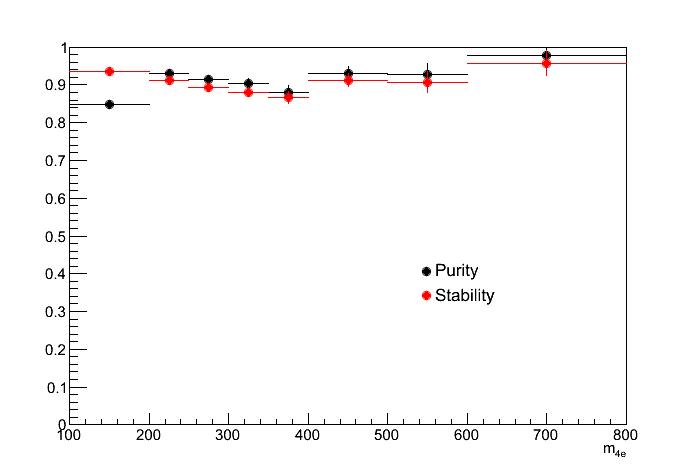
\includegraphics[width=\cmsFigWidth]{Figures/Unfolding/BinMigration/PurityStability_4e_Mass}     
%%     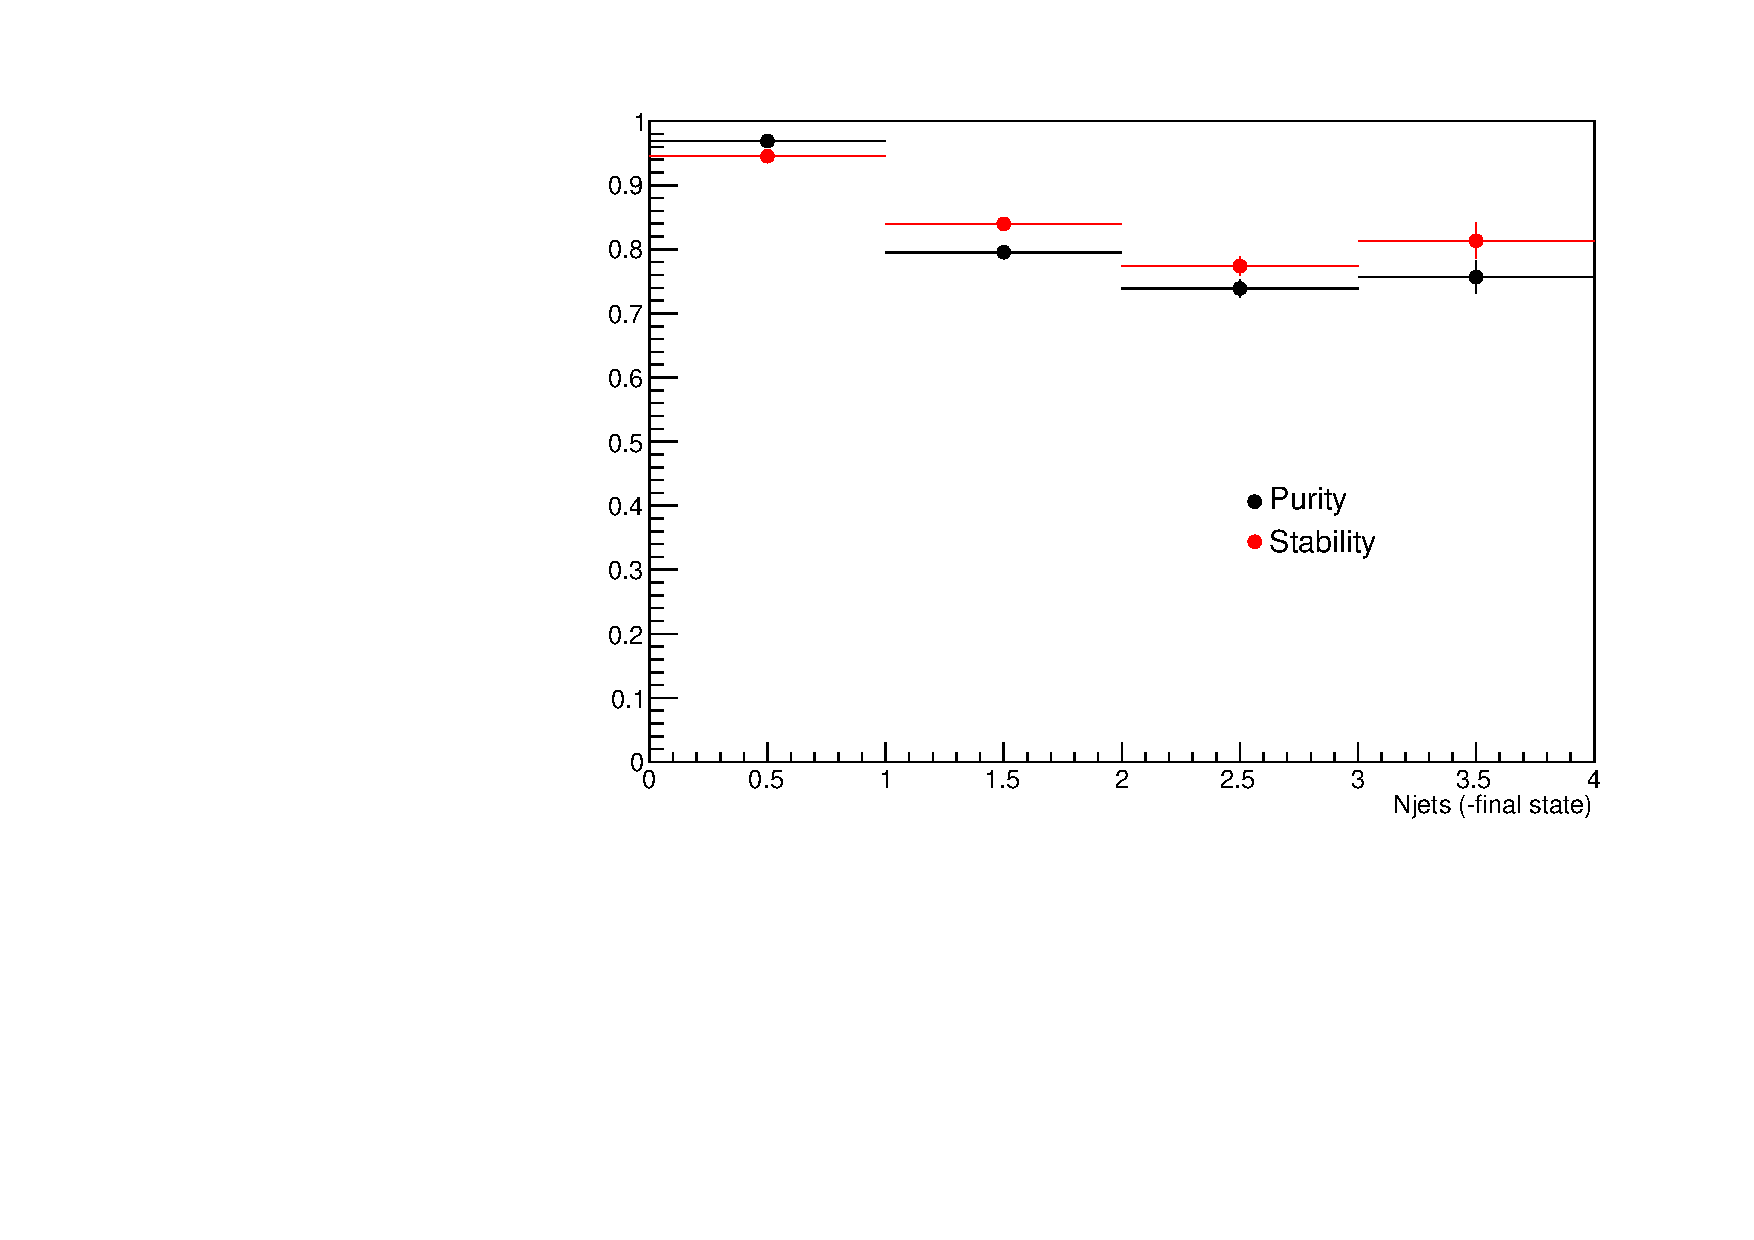
\includegraphics[width=\cmsFigWidth]{Figures/Unfolding/BinMigration/PurityStability_4e_Jets}
%%    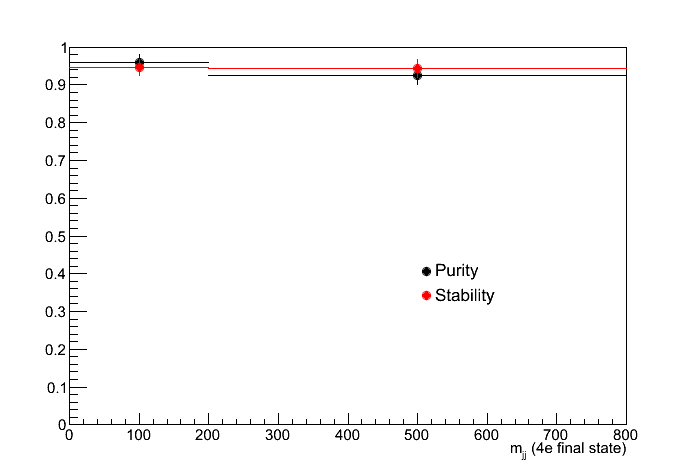
\includegraphics[width=\cmsFigWidth]{Figures/Unfolding/BinMigration/PurityStability_4e_Mjj}
%%    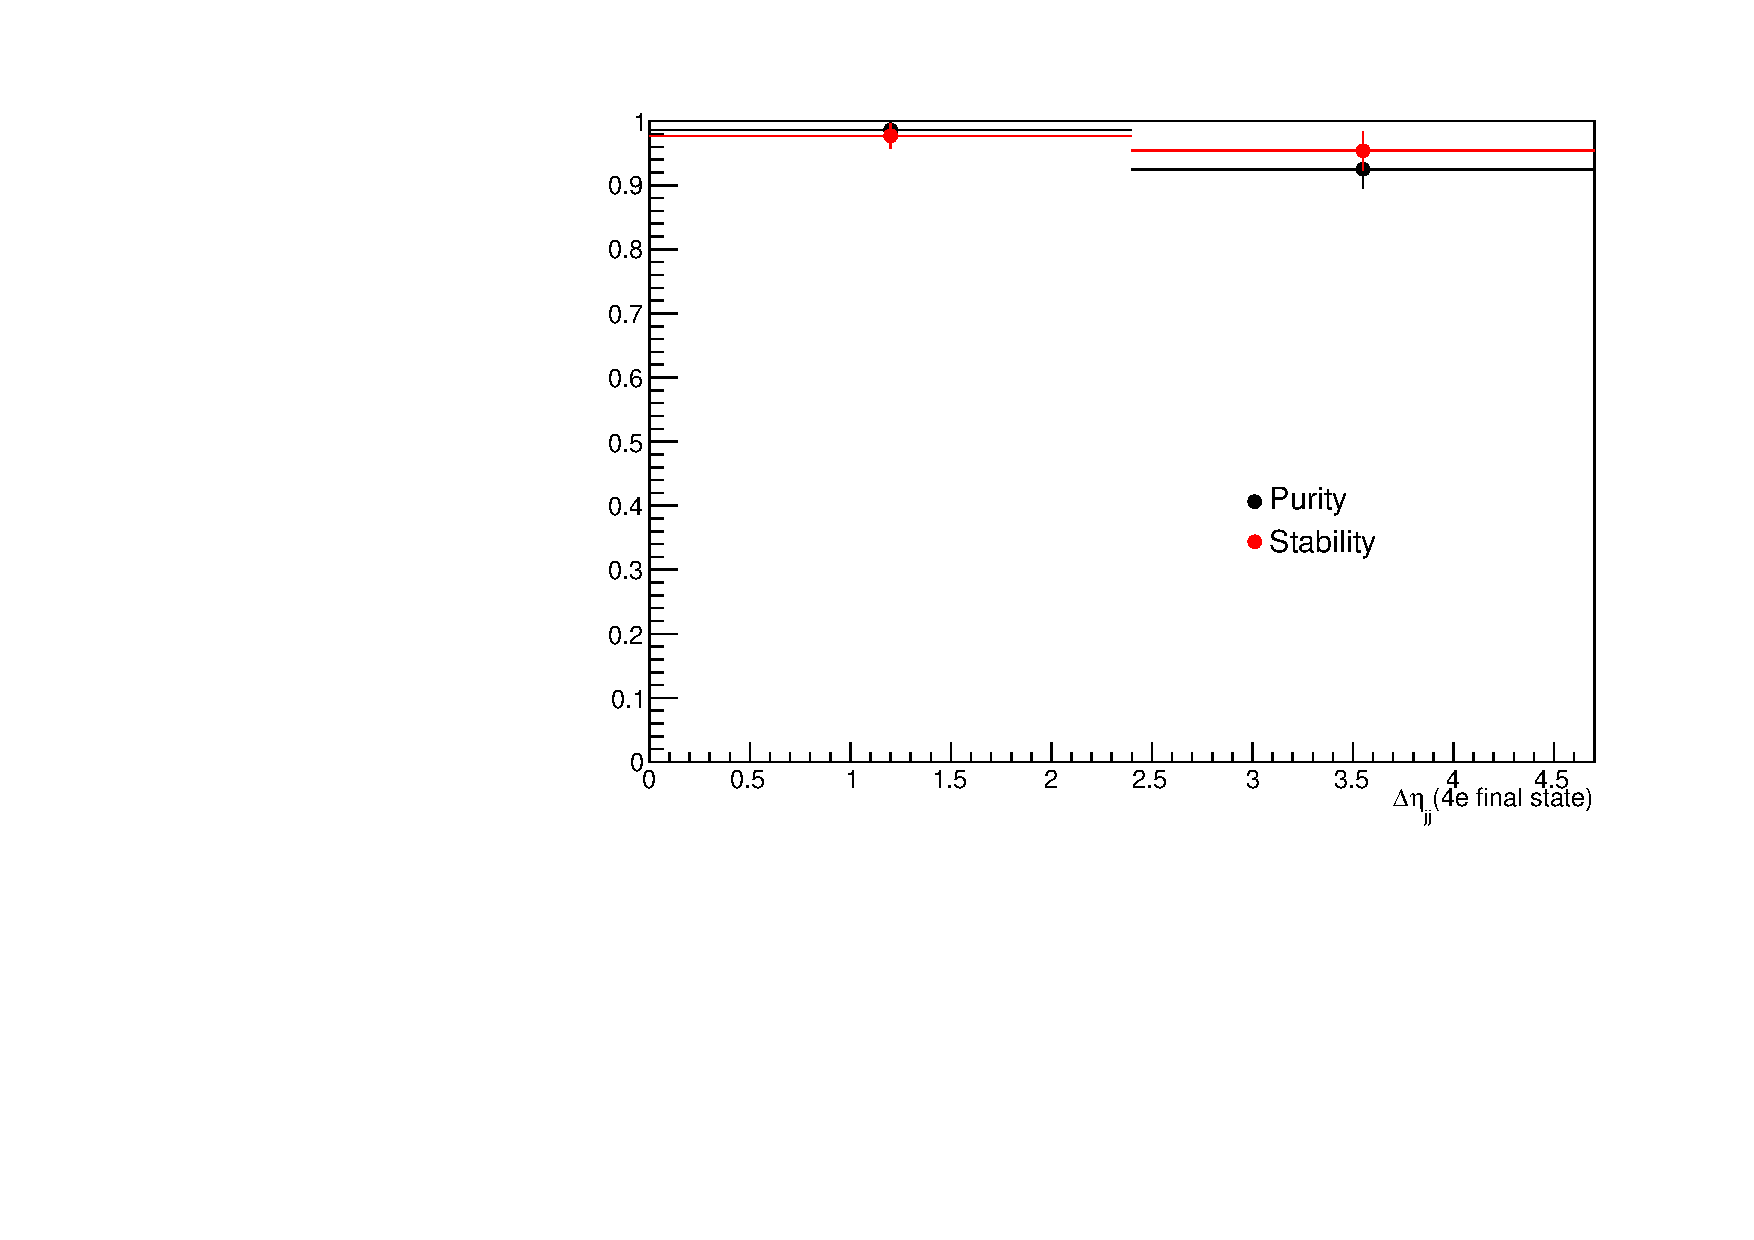
\includegraphics[width=\cmsFigWidth]{Figures/Unfolding/BinMigration/PurityStability_4e_Deta}
%%      \caption{Purity and stability as a function of the invariant mass of the 4-lepton system (top left), the number of jets in the event (top right), the invariant mass of the two most energetic jets (bottom left) and the $\Delta\eta$ between them (bottom right) for the $4e$ final state.}
%%     \label{fig:ps_4e}
%%   \end{center}
%% \end{figure}
%% \begin{figure}[hbtp]
%%   \begin{center}
%%     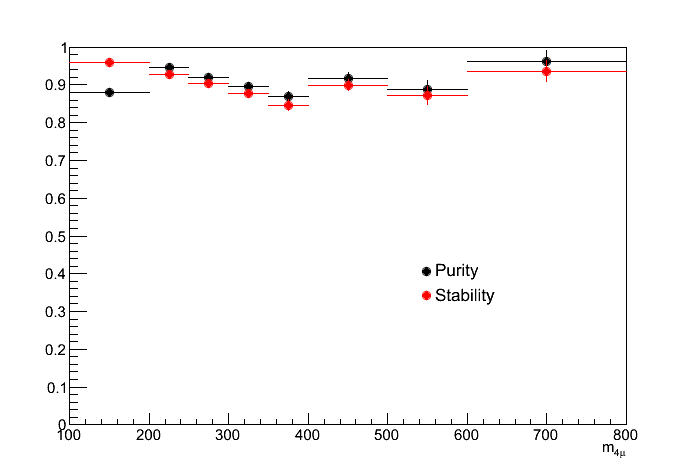
\includegraphics[width=\cmsFigWidth]{Figures/Unfolding/BinMigration/PurityStability_4m_Mass}     
%%     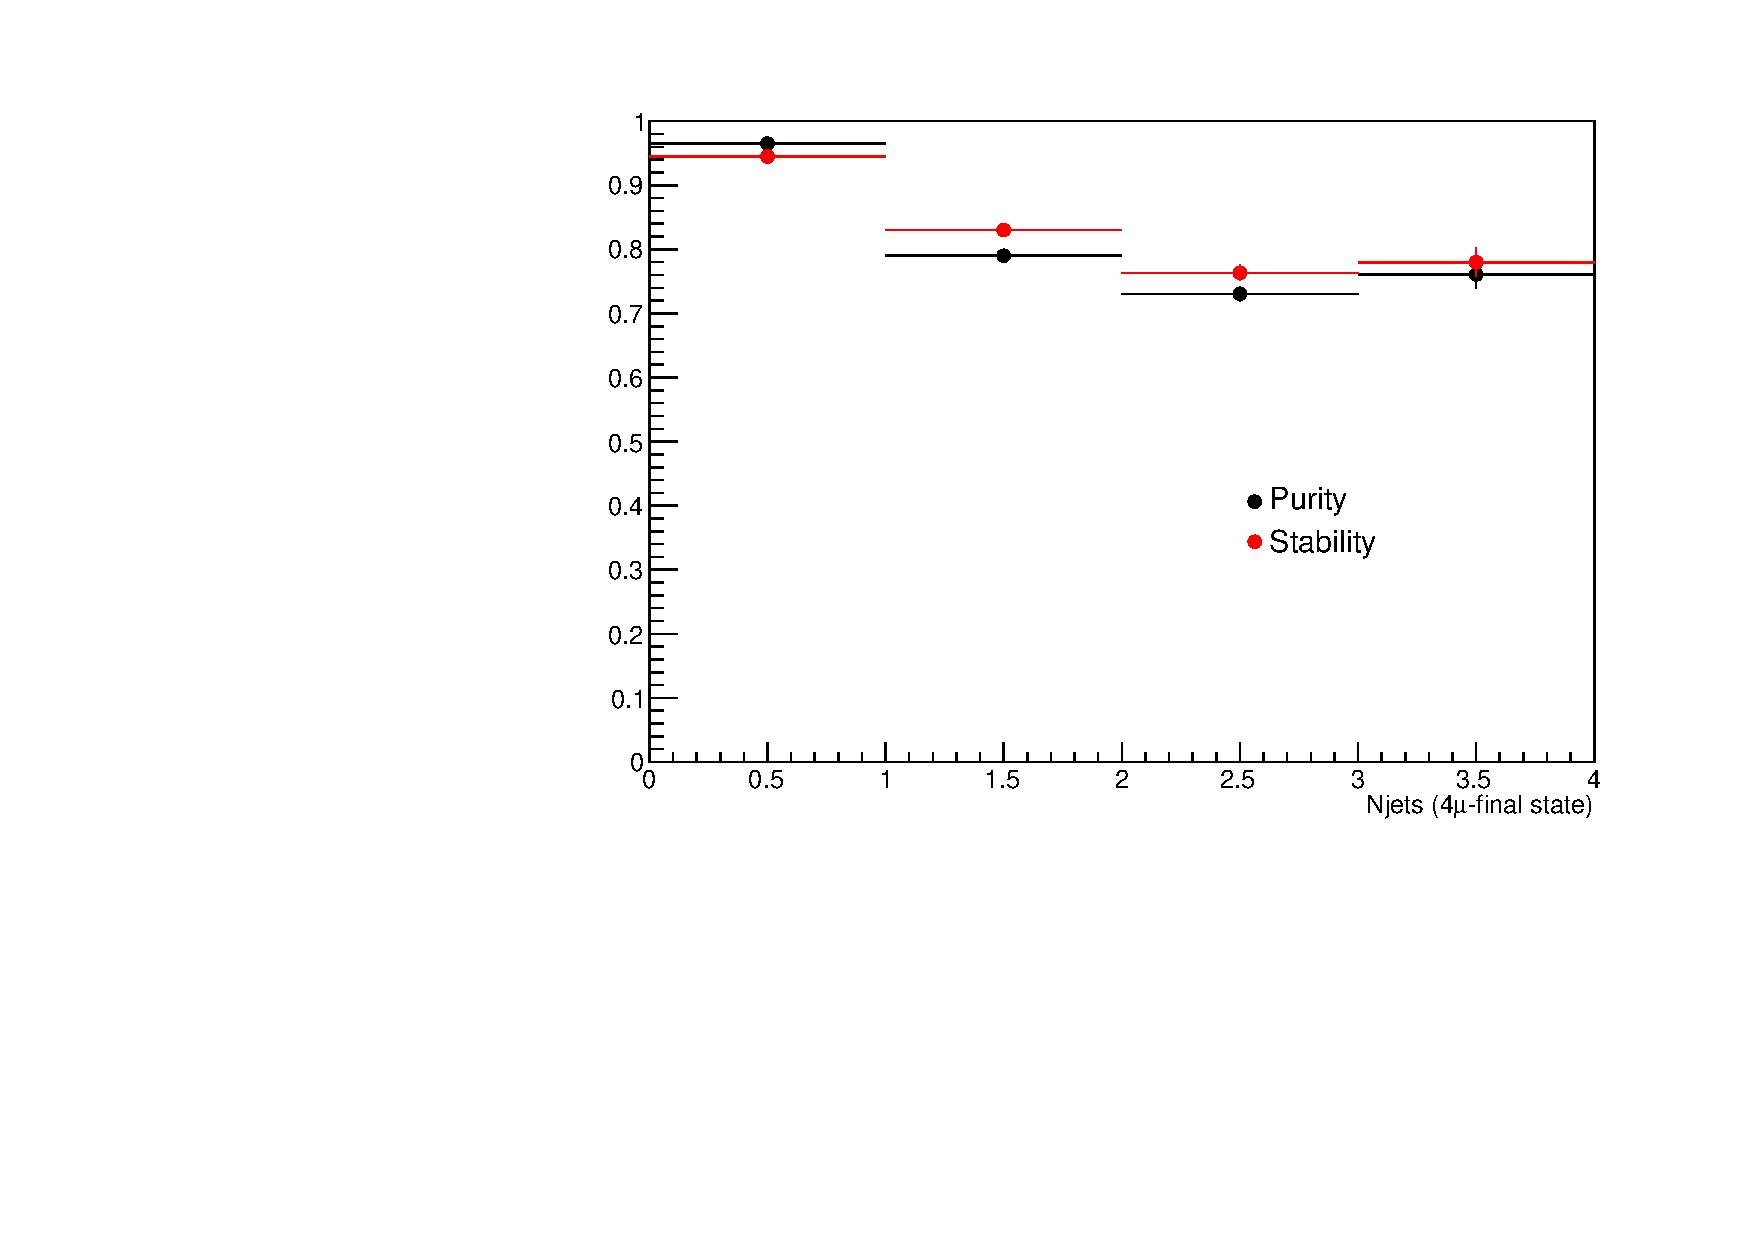
\includegraphics[width=\cmsFigWidth]{Figures/Unfolding/BinMigration/PurityStability_4m_Jets}
%%     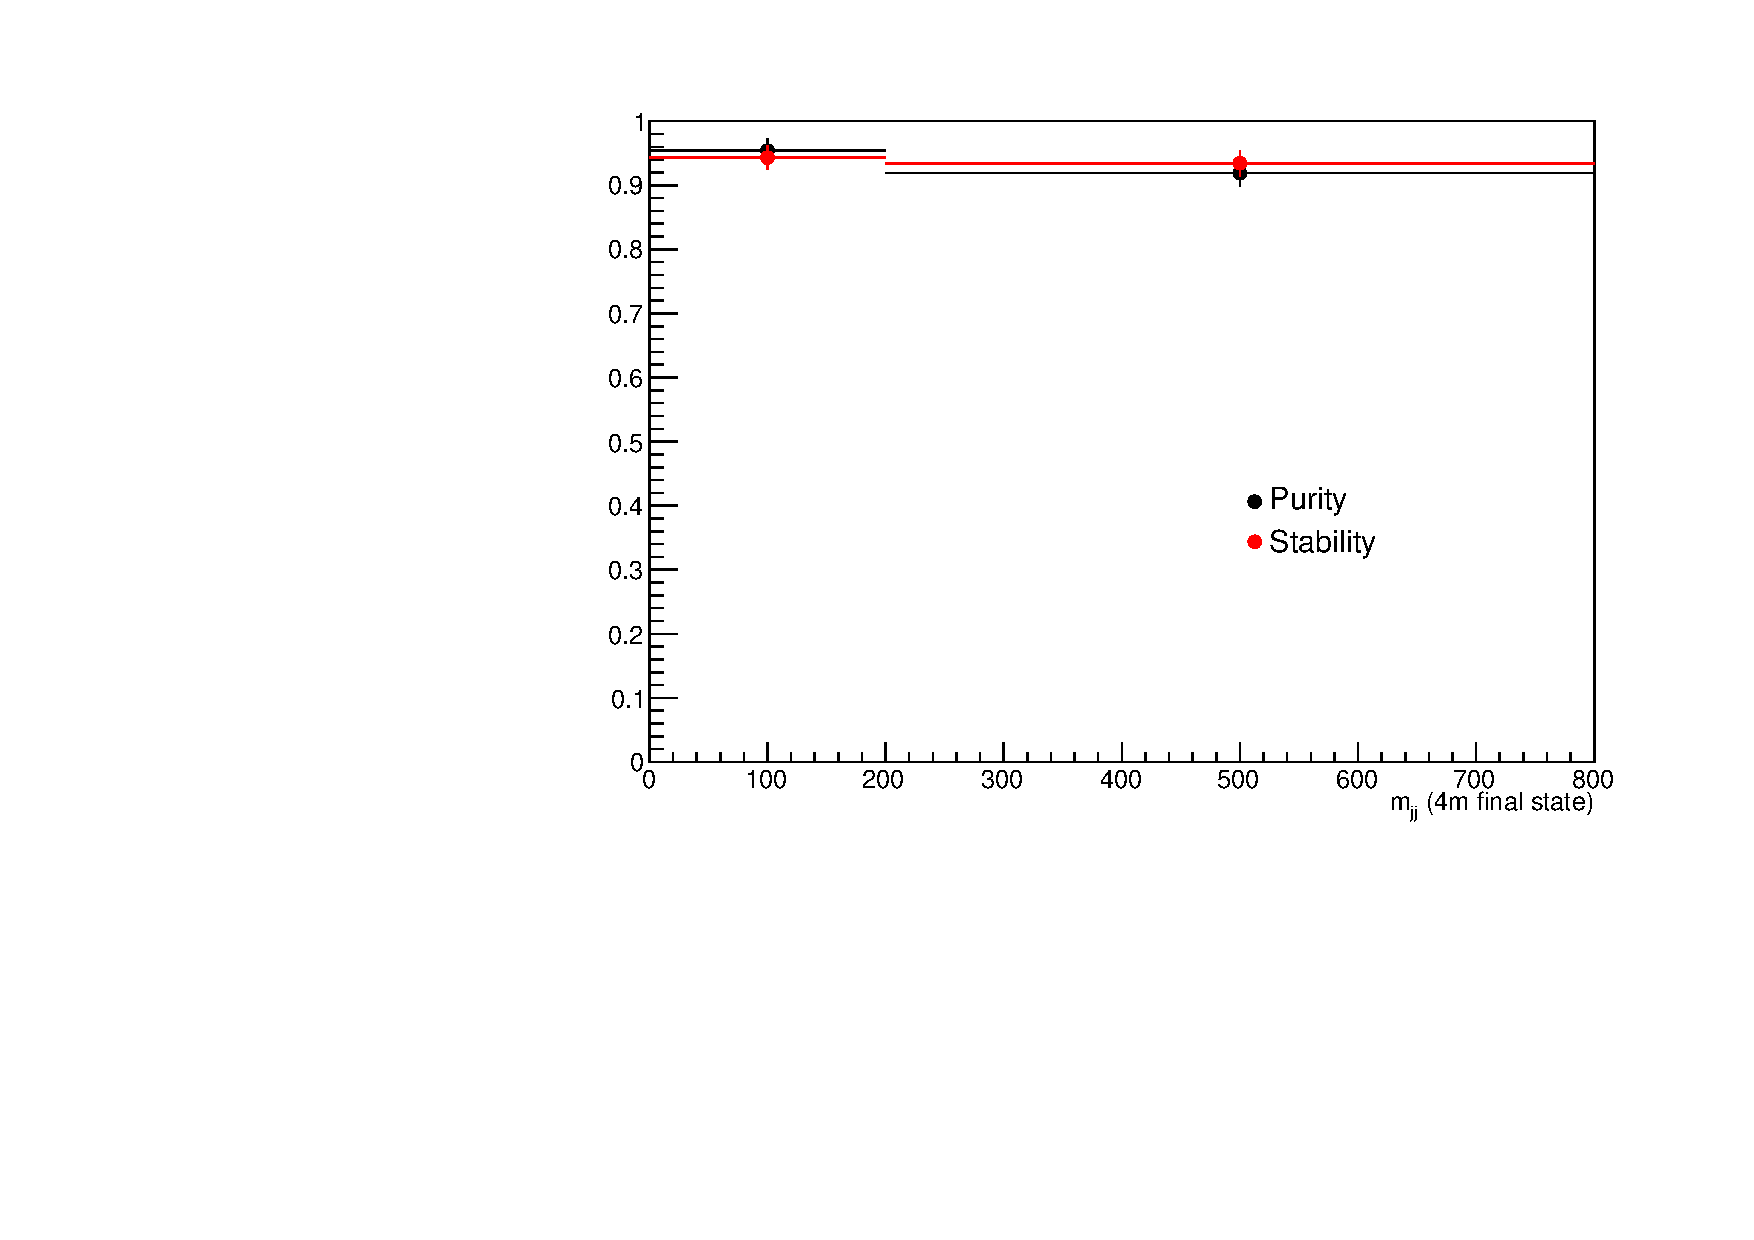
\includegraphics[width=\cmsFigWidth]{Figures/Unfolding/BinMigration/PurityStability_4m_Mjj}
%%    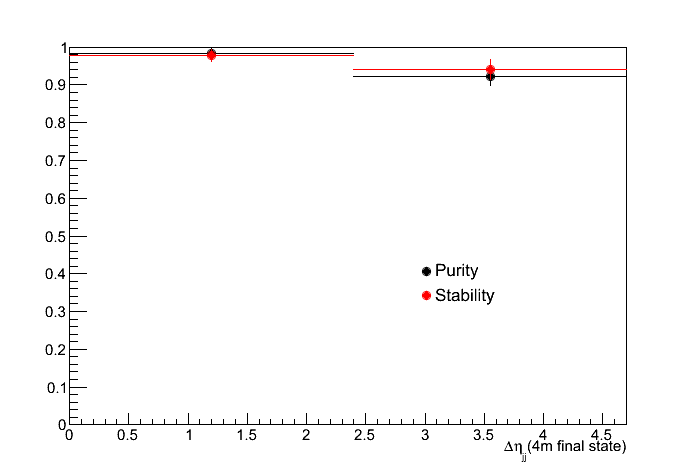
\includegraphics[width=\cmsFigWidth]{Figures/Unfolding/BinMigration/PurityStability_4m_Deta}
%%      \caption{Purity and stability as a function of the invariant mass of the 4-lepton system (top left), the number of jets in the event (top right), the invariant mass of the two most energetic jets (bottom left) and the $\Delta\eta$ between them (bottom right) for the $4\mu$ final state.}
%%     \label{fig:ps_4m}
%%   \end{center}
%% \end{figure}
%% \begin{figure}[hbtp]
%%   \begin{center}
%%     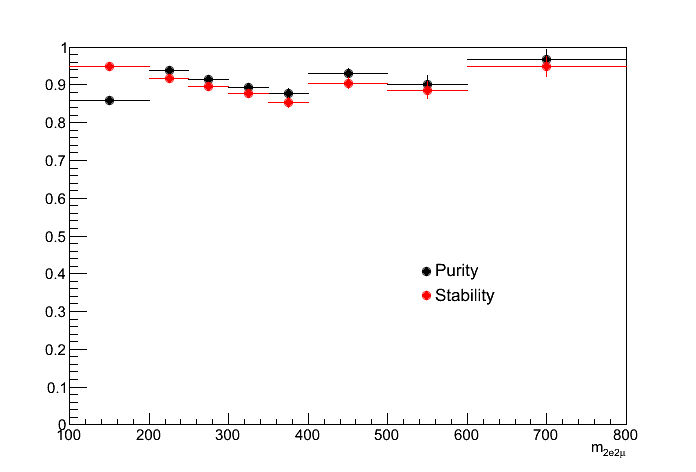
\includegraphics[width=\cmsFigWidth]{Figures/Unfolding/BinMigration/PurityStability_2e2m_Mass}     
%%     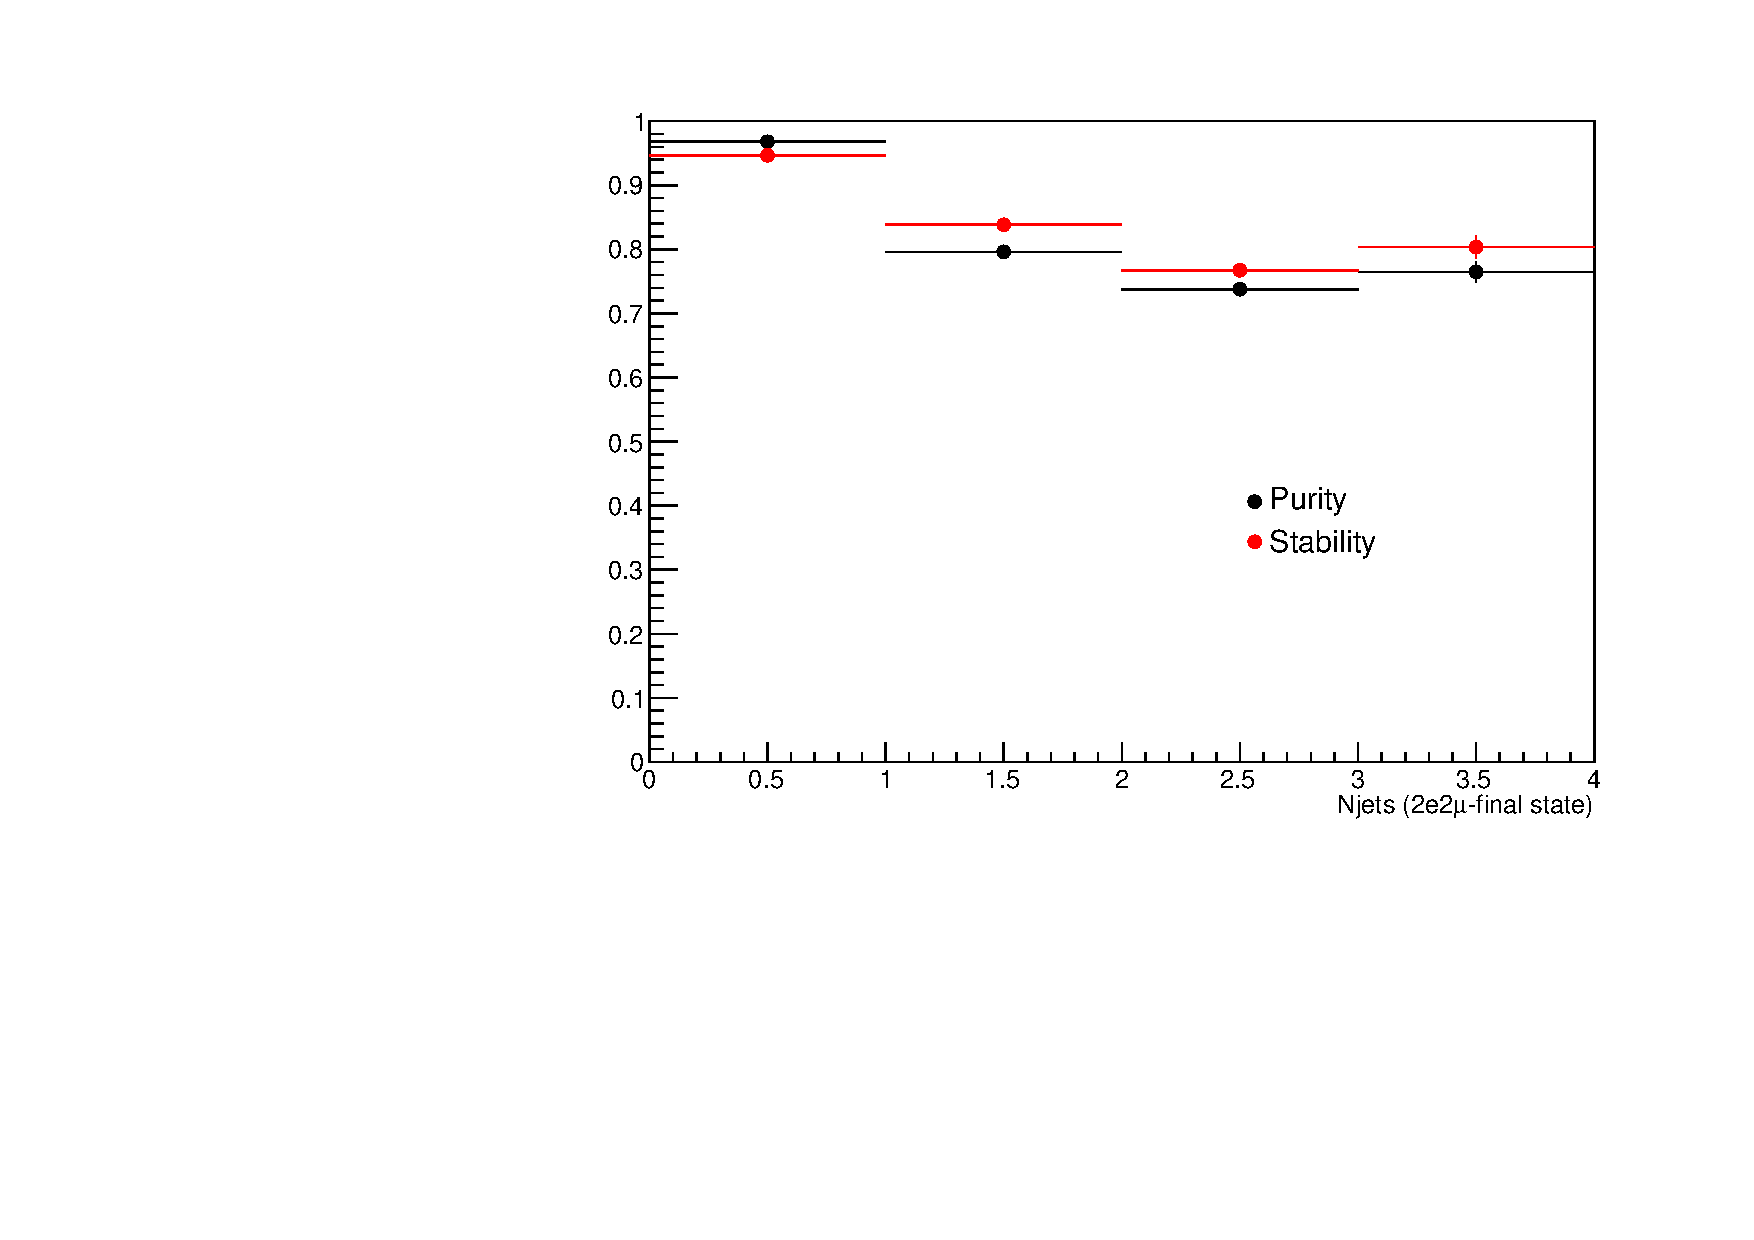
\includegraphics[width=\cmsFigWidth]{Figures/Unfolding/BinMigration/PurityStability_2e2m_Jets}
%%    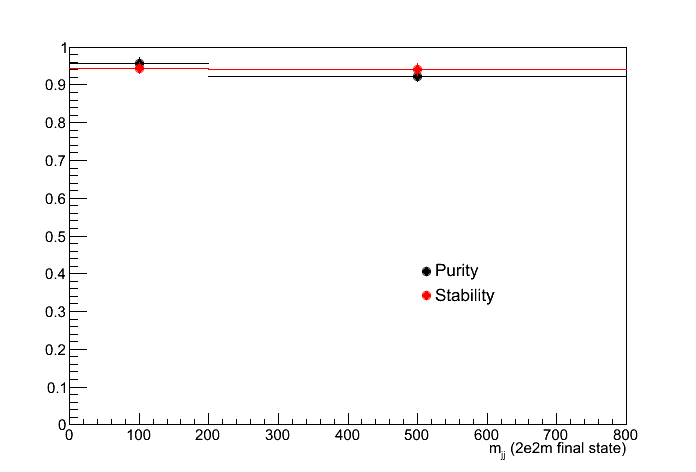
\includegraphics[width=\cmsFigWidth]{Figures/Unfolding/BinMigration/PurityStability_2e2m_Mjj}
%%    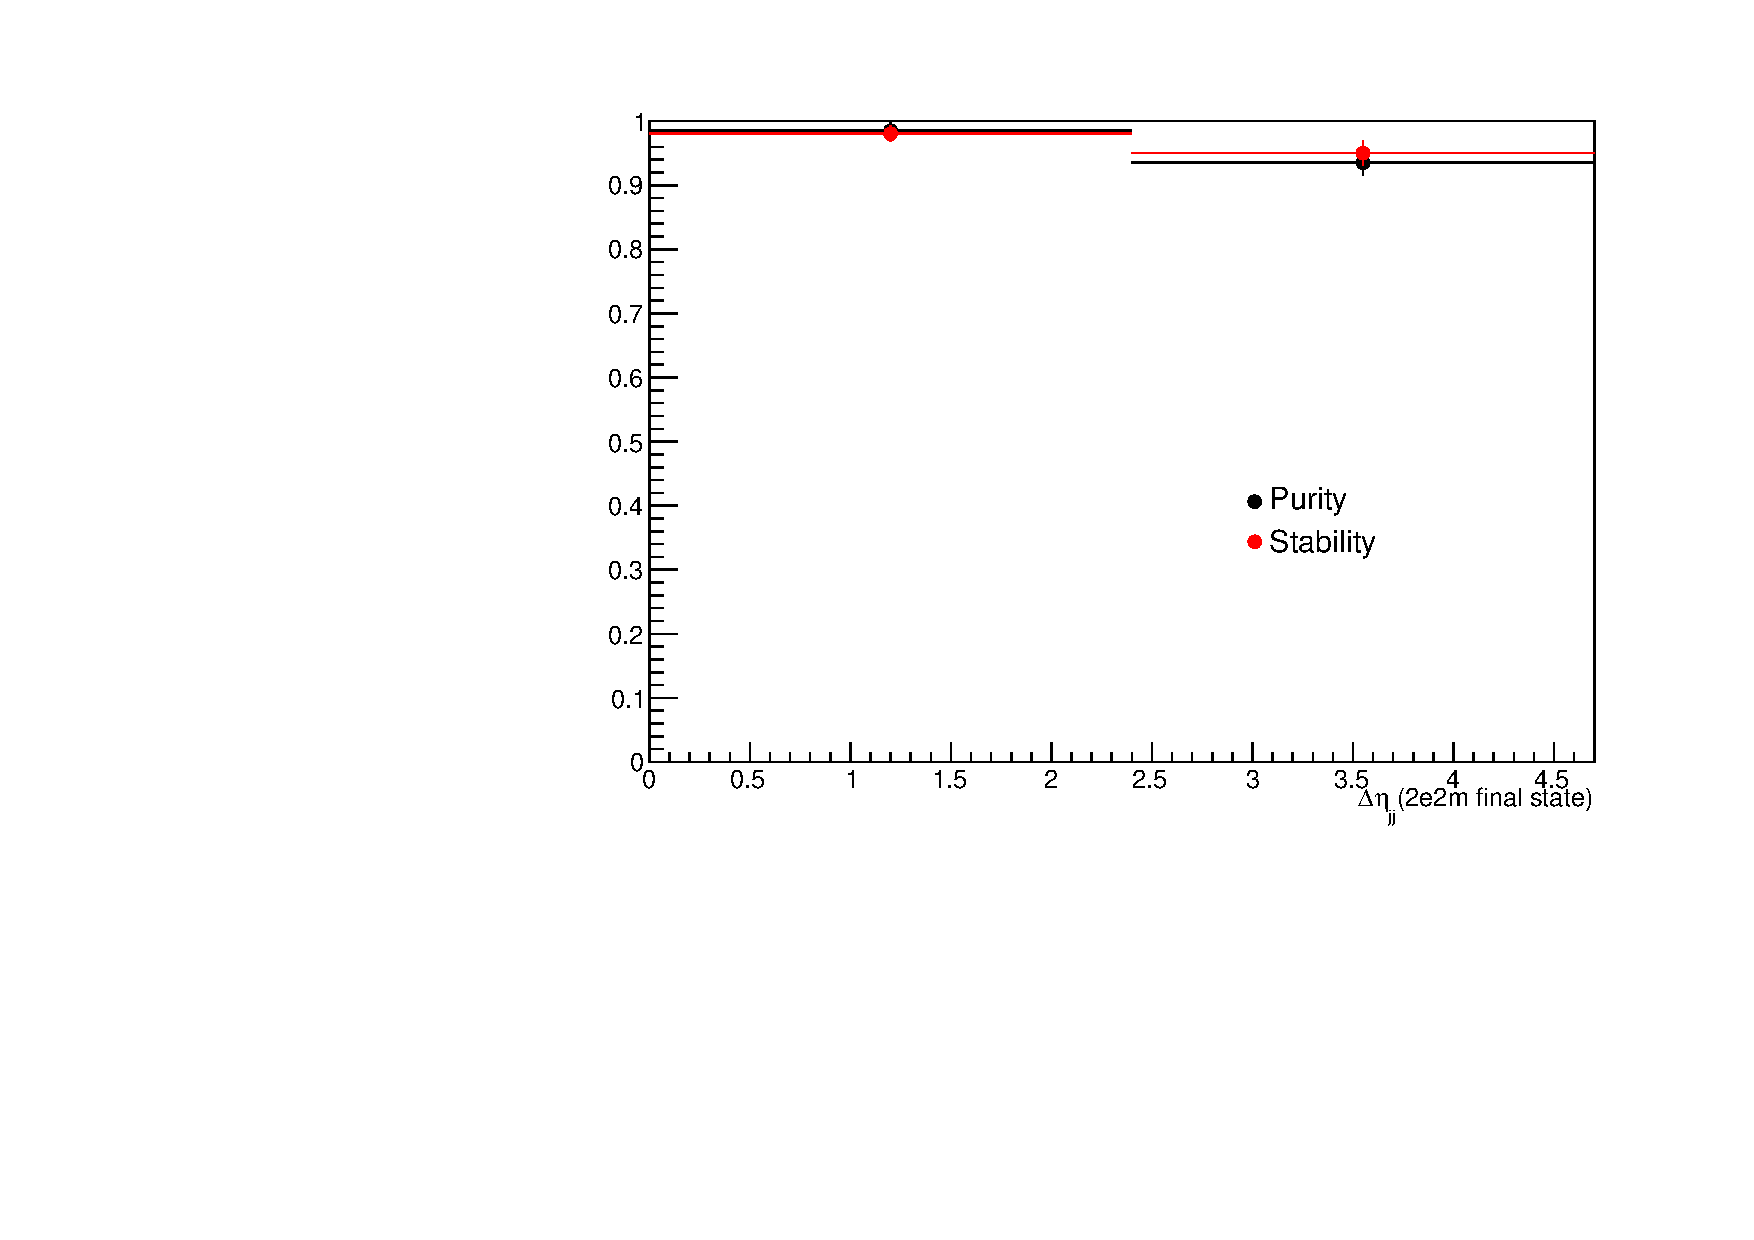
\includegraphics[width=\cmsFigWidth]{Figures/Unfolding/BinMigration/PurityStability_2e2m_Deta}
%%      \caption{Purity and stability as a function of the invariant mass of the 4-lepton system (top left), the number of jets in the event (top right), the invariant mass of the two most energetic jets (bottom left) and the $\Delta\eta$ between them (bottom right) for the $2e2\mu$ final state.}
%%     \label{fig:ps_2e2m}
%%   \end{center}
%% \end{figure}

%% \begin{figure}[hbtp]
%%   \begin{center}
%%     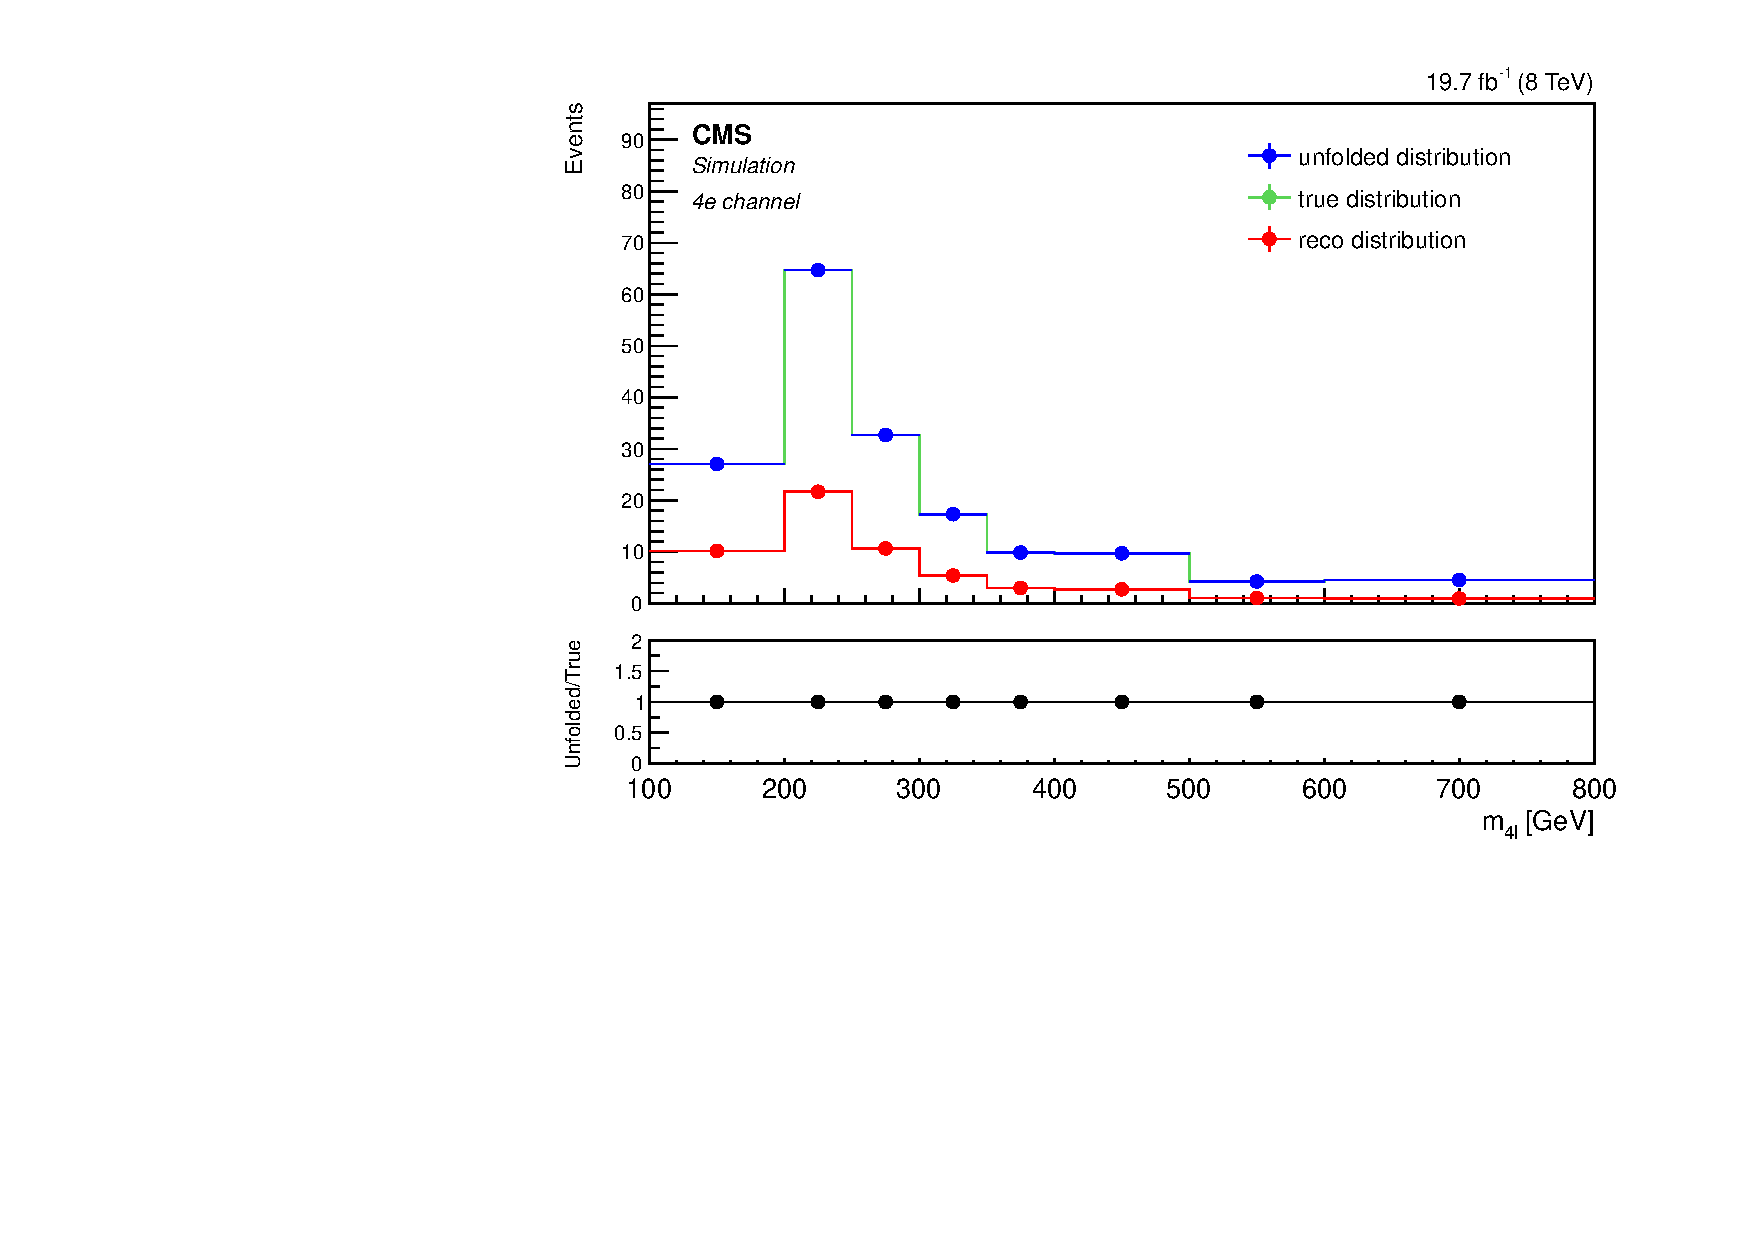
\includegraphics[width=\cmsFigWidth]{Figures/Unfolding/MCTests/Mass_ZZTo4e_MadMatrix_MadDistr_FullSample}     
%%     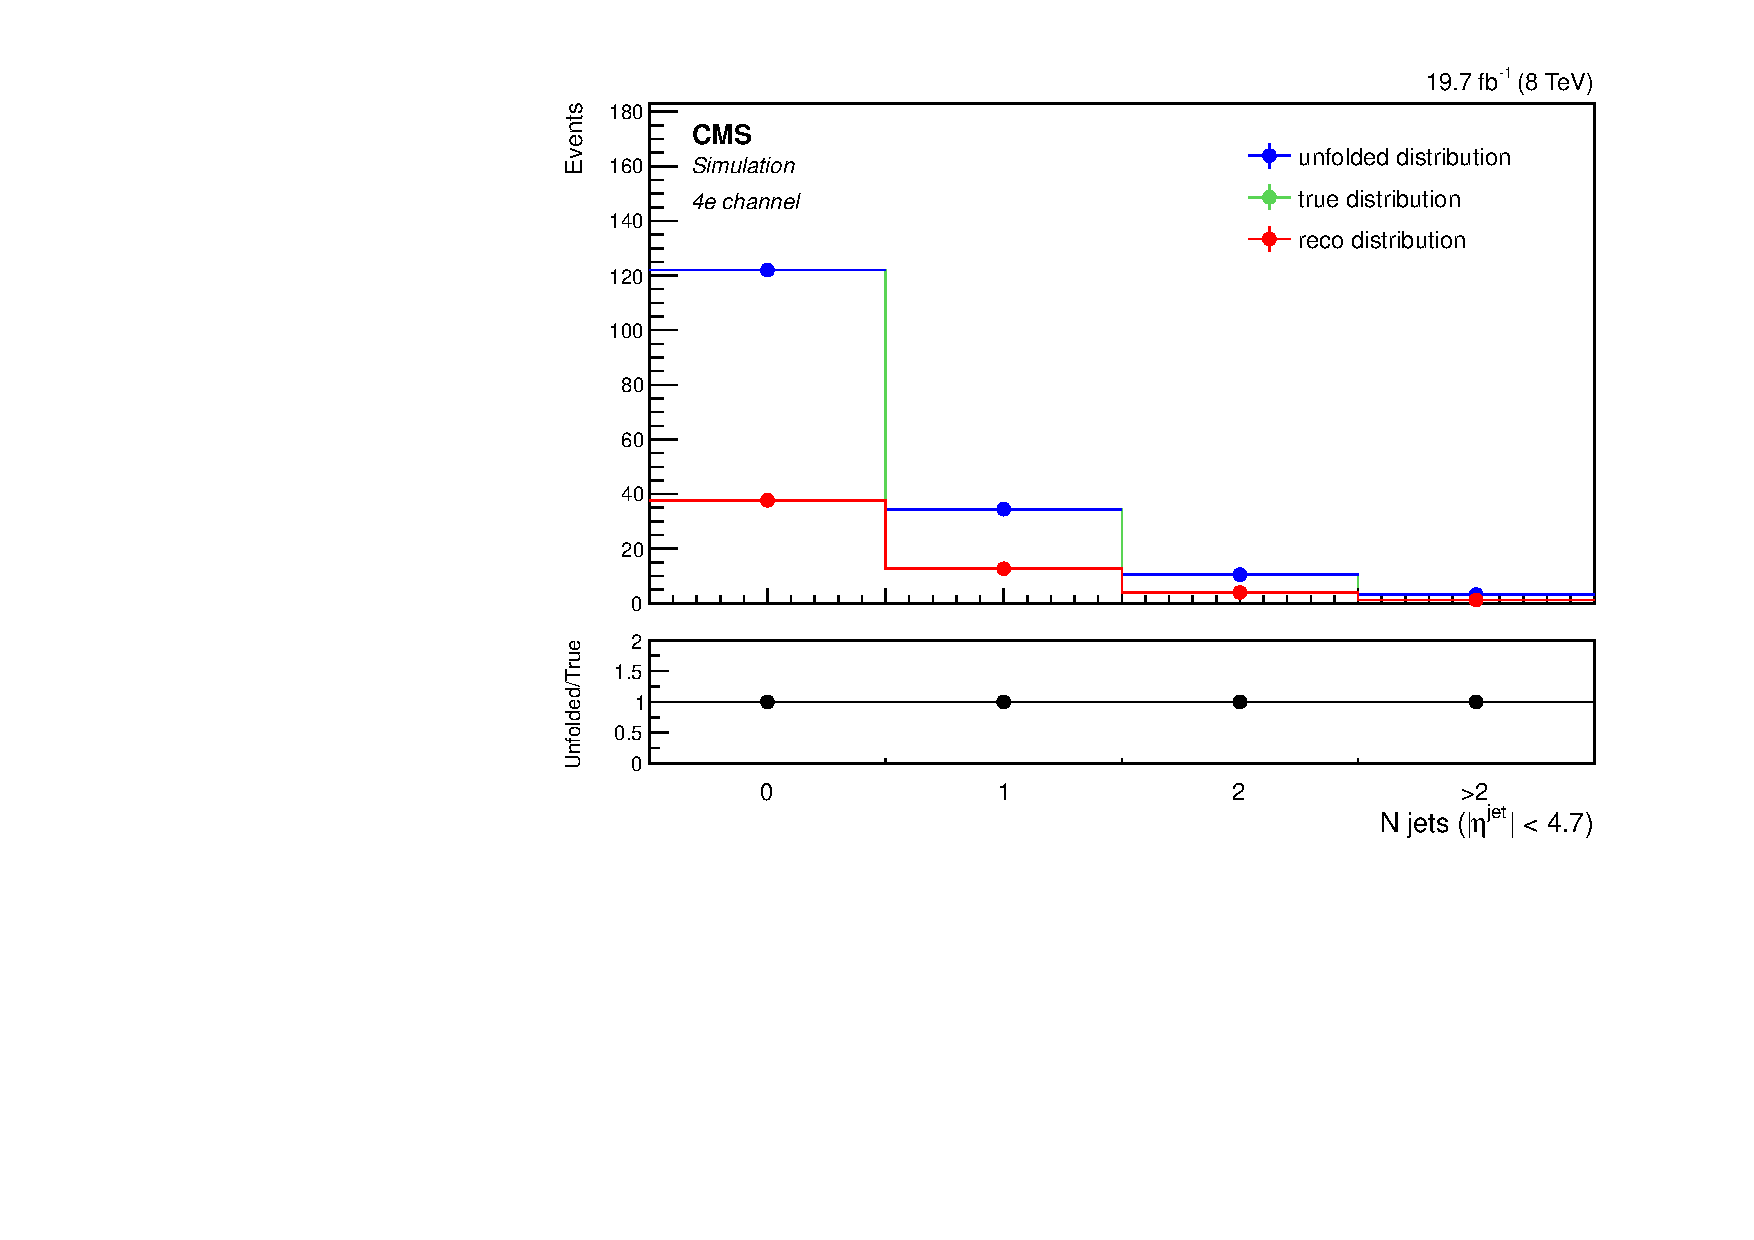
\includegraphics[width=\cmsFigWidth]{Figures/Unfolding/MCTests/Jets_ZZTo4e_MadMatrix_MadDistr_FullSample}
%%      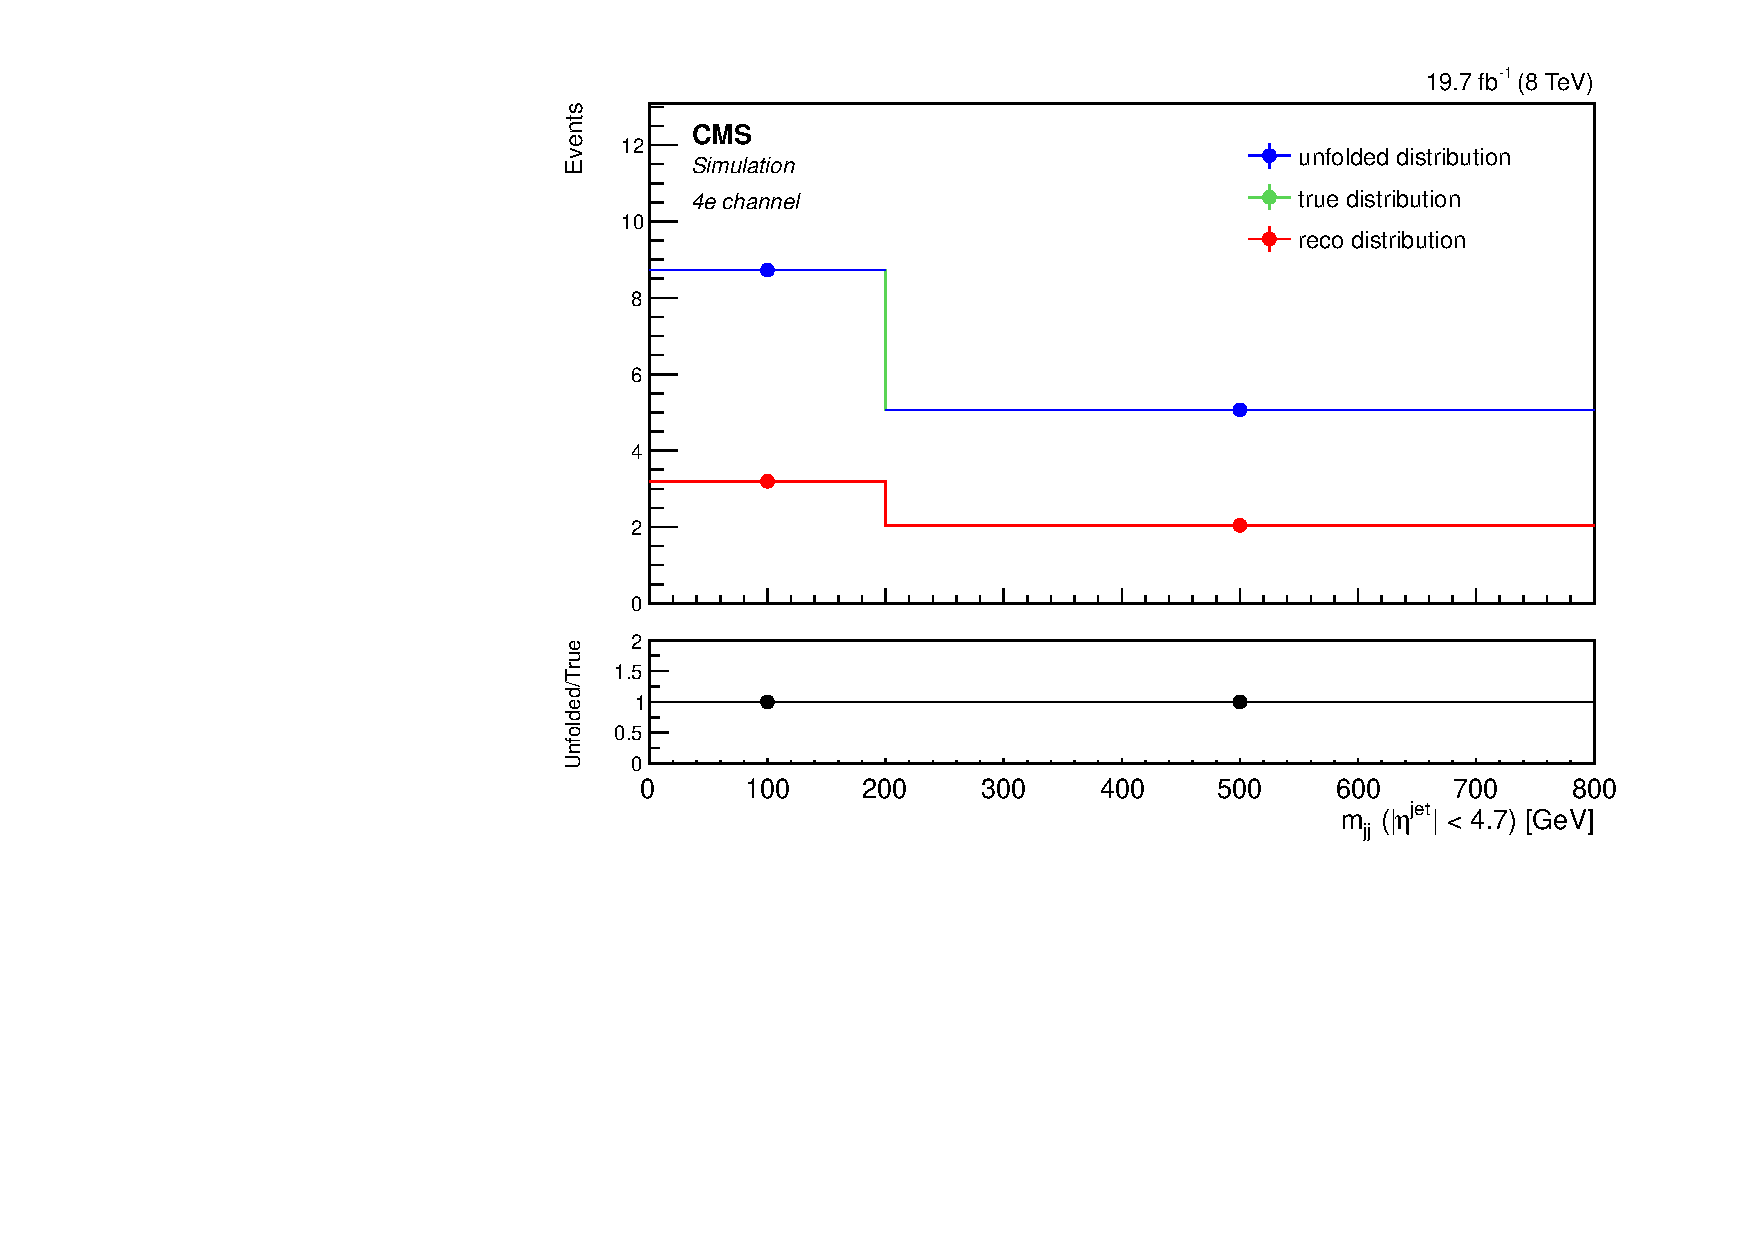
\includegraphics[width=\cmsFigWidth]{Figures/Unfolding/MCTests/Mjj_ZZTo4e_MadMatrix_MadDistr_FullSample}
%%      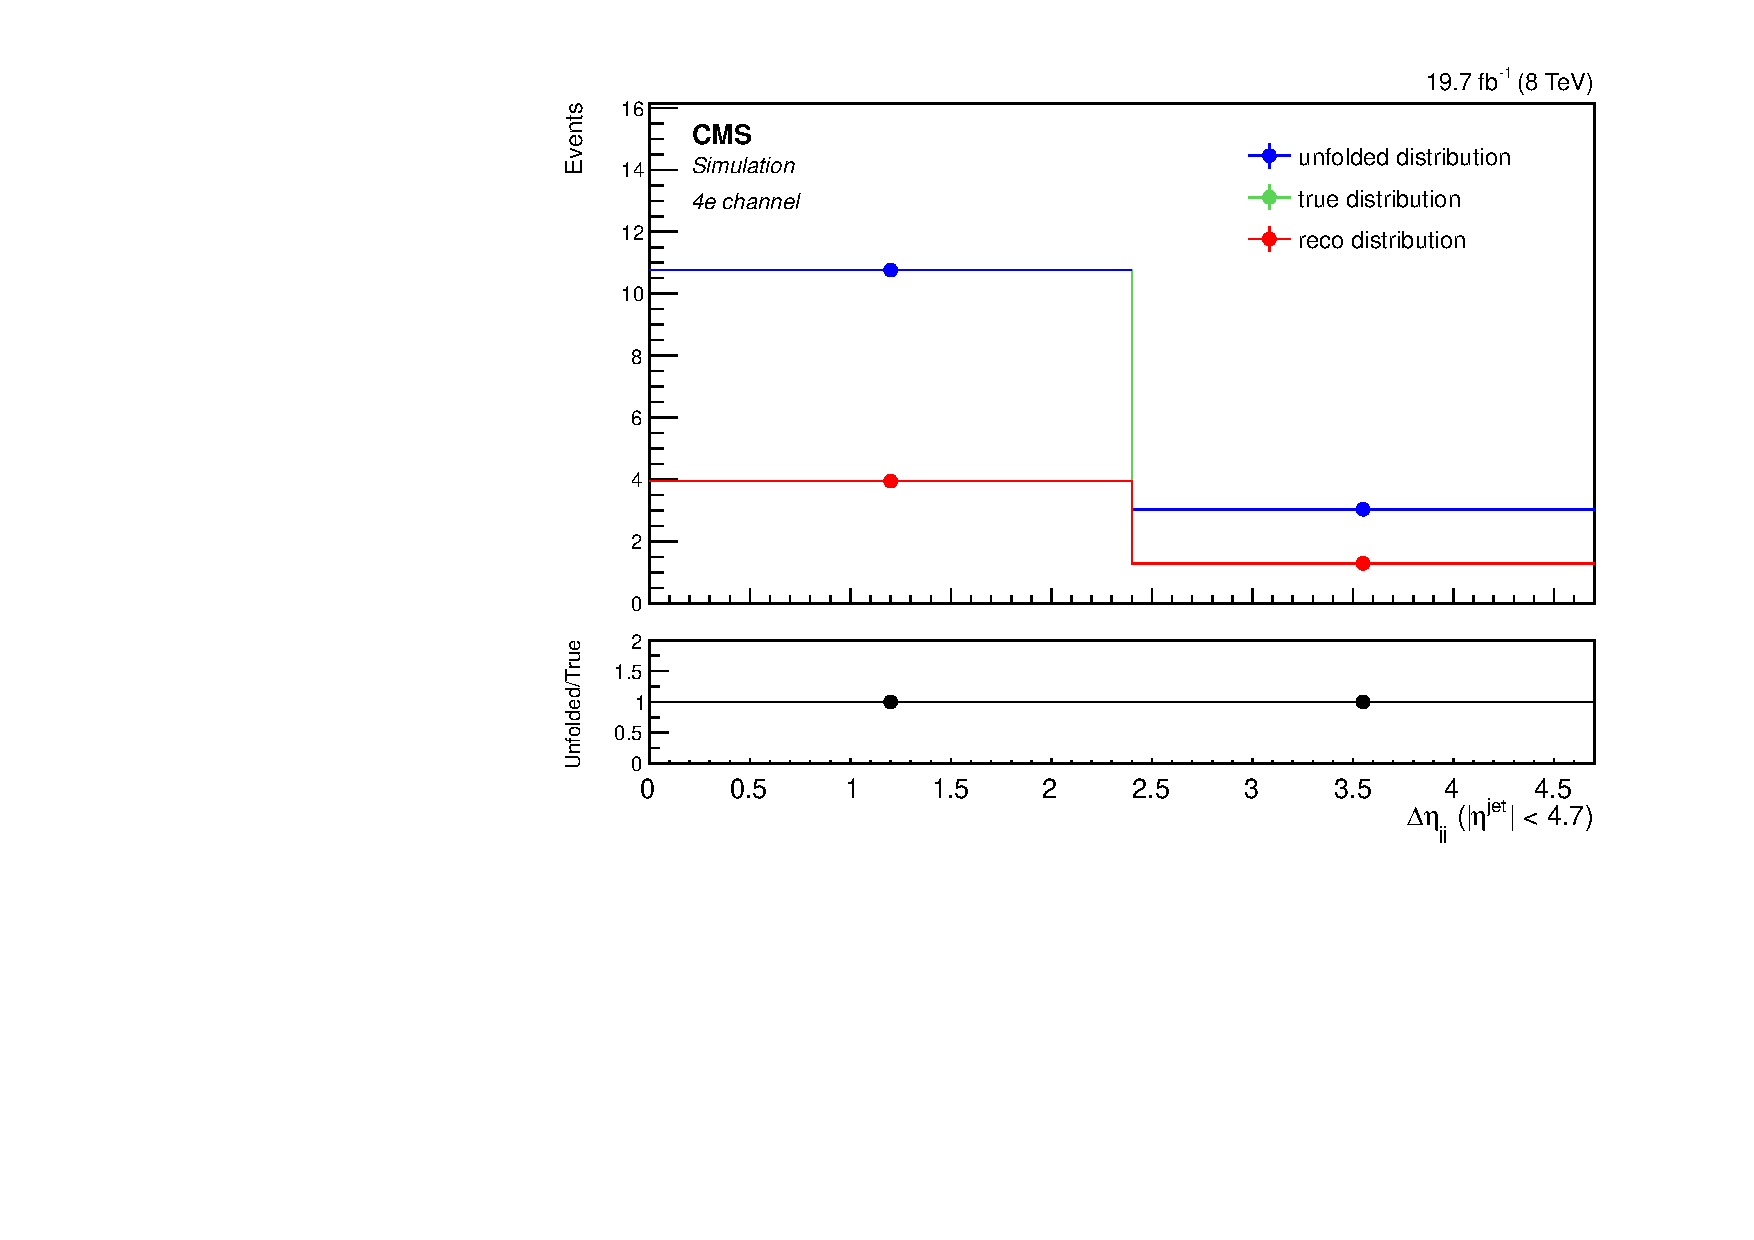
\includegraphics[width=\cmsFigWidth]{Figures/Unfolding/MCTests/Deta_ZZTo4e_MadMatrix_MadDistr_FullSample}
%%      \caption{Unfolding test: \texttt{MadGraph} matrix applied on \texttt{MadGraph} distribution, using the full set. Results are reported as a function of 
%%  the invariant mass of the 4-lepton system (top left), the number of jets in the event (top right), the invariant mass of the two most energetic jets (bottom left) and the $\Delta\eta$ between them (bottom right) for the $4e$ final state.}
%%     \label{fig:FullMad_4e}
%%   \end{center}
%% \end{figure}
%% \begin{figure}[hbtp]
%%   \begin{center}
%%     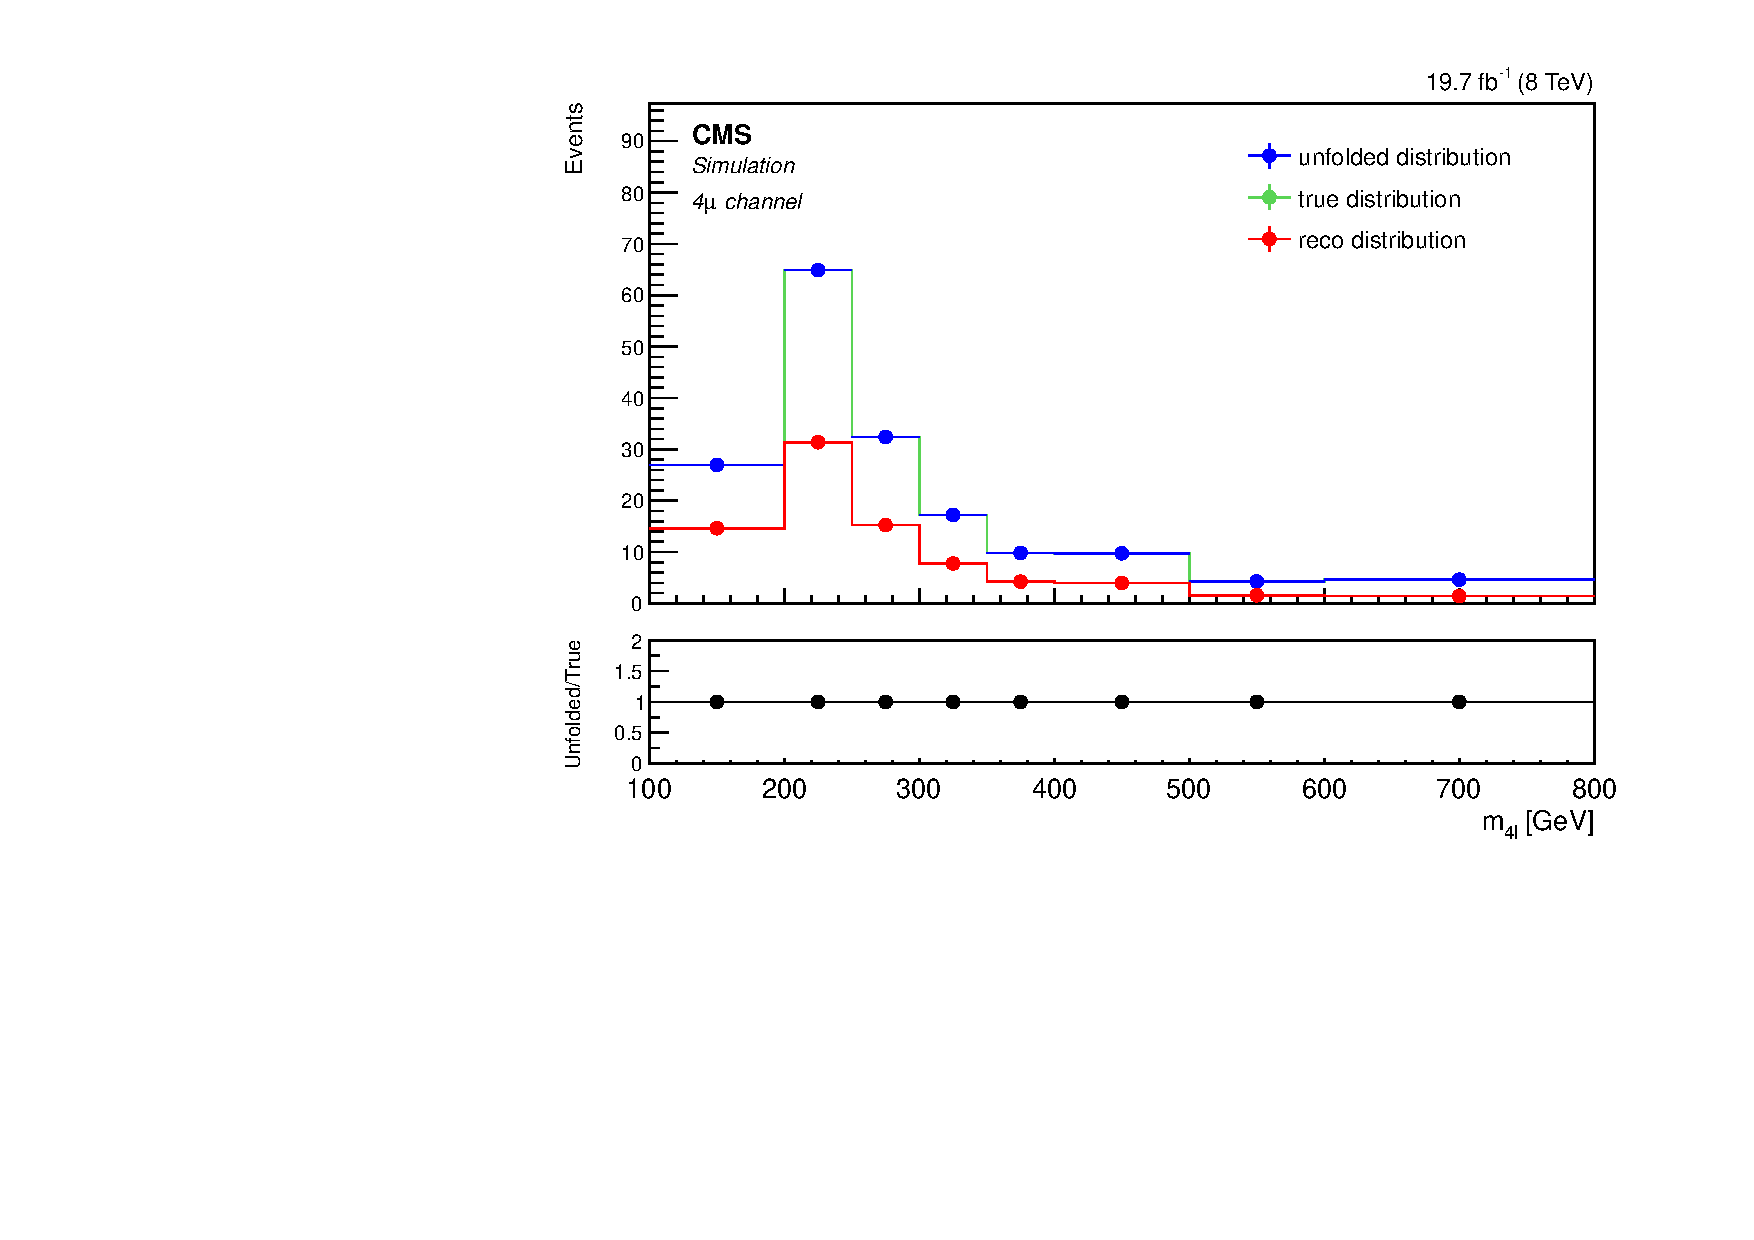
\includegraphics[width=\cmsFigWidth]{Figures/Unfolding/MCTests/Mass_ZZTo4m_MadMatrix_MadDistr_FullSample}     
%%     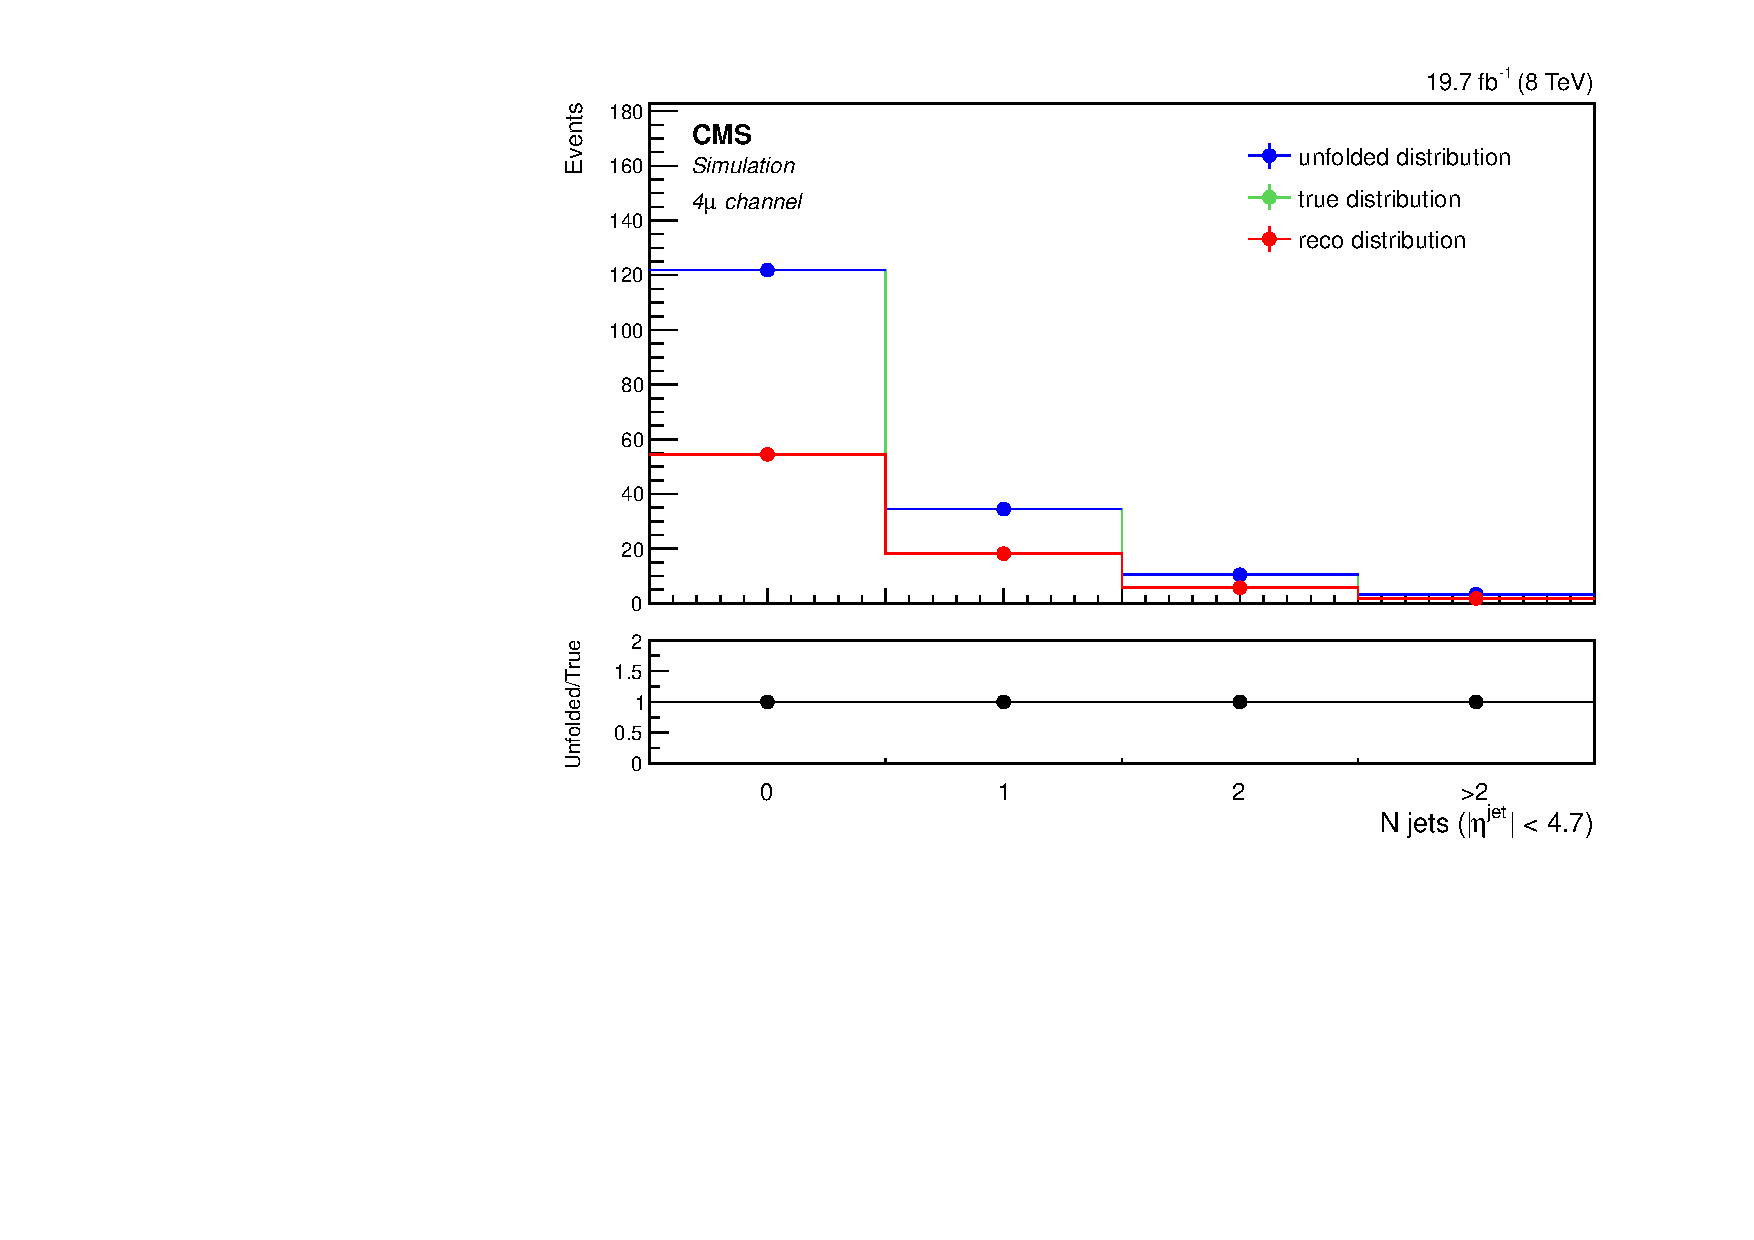
\includegraphics[width=\cmsFigWidth]{Figures/Unfolding/MCTests/Jets_ZZTo4m_MadMatrix_MadDistr_FullSample}
%%      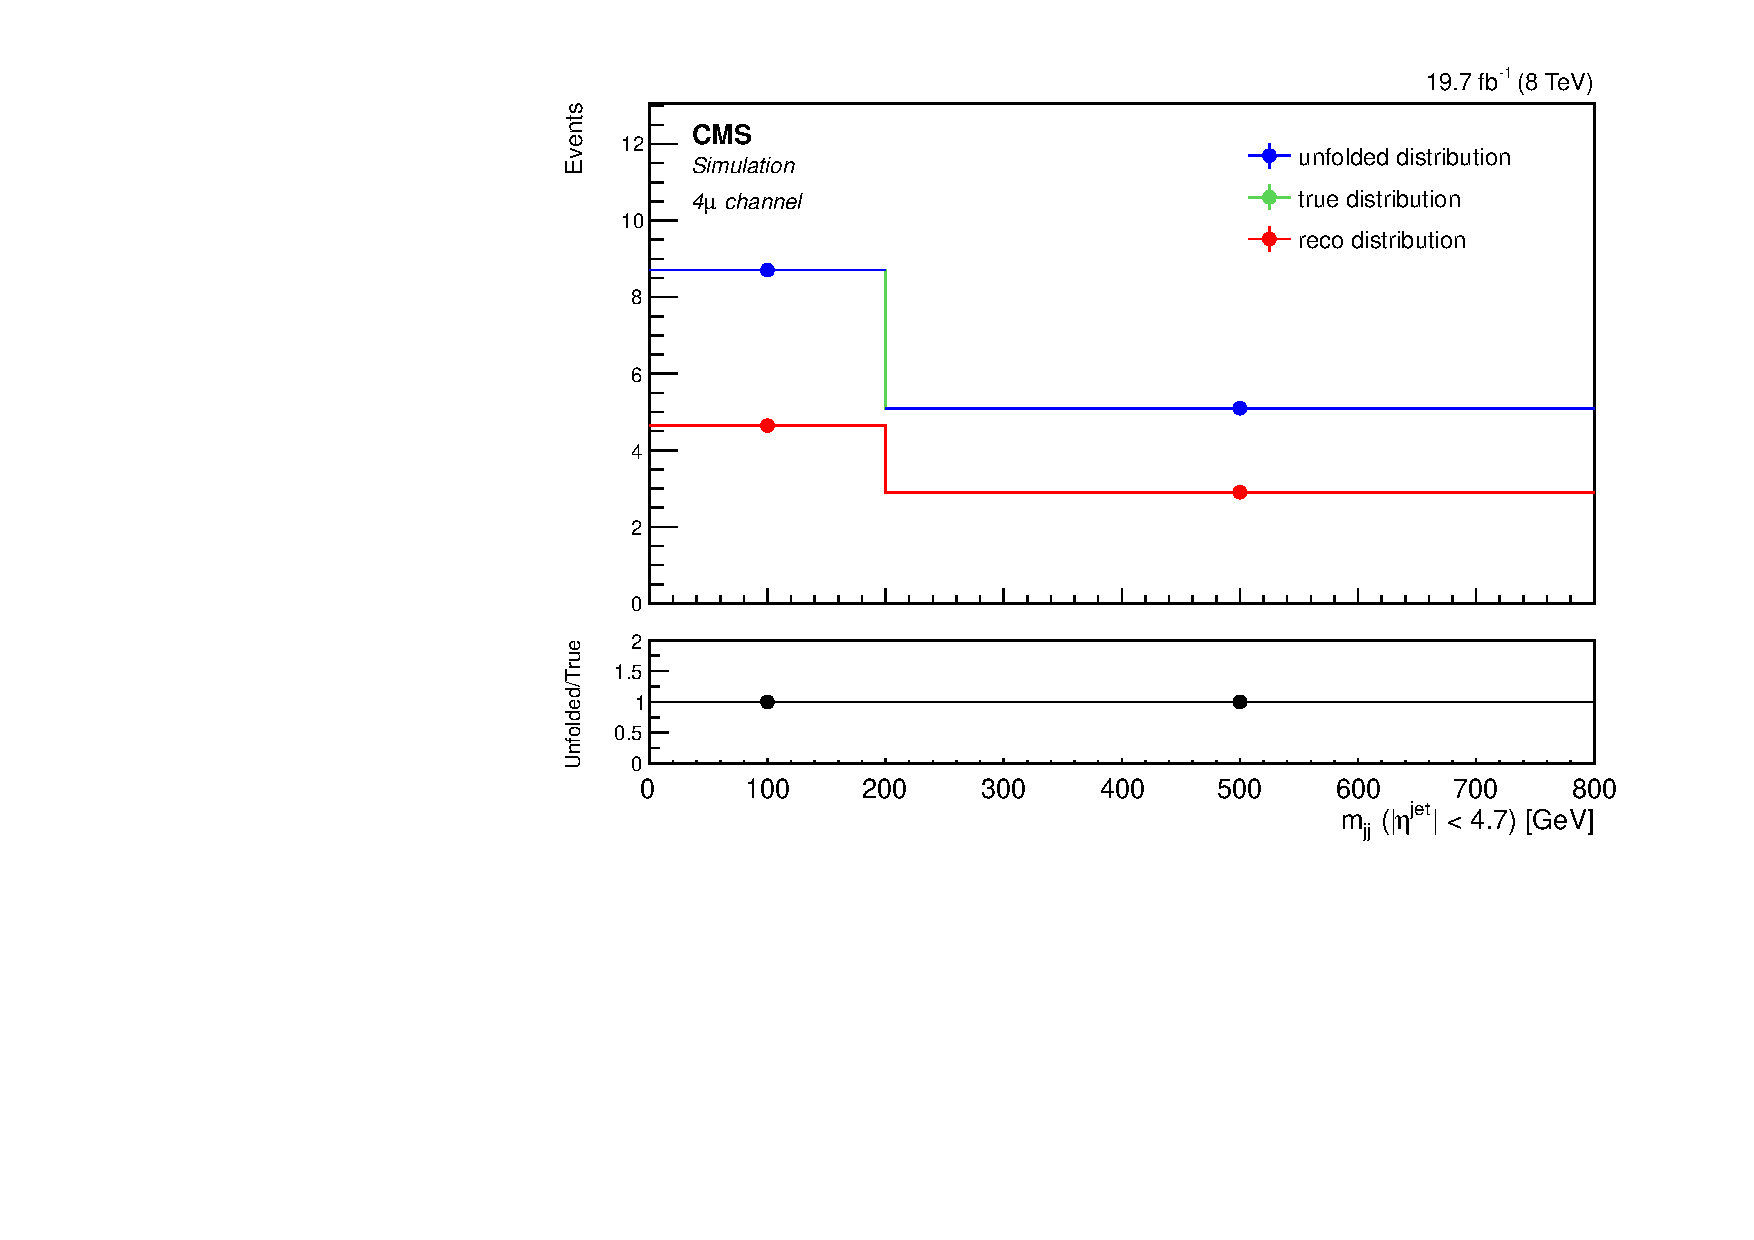
\includegraphics[width=\cmsFigWidth]{Figures/Unfolding/MCTests/Mjj_ZZTo4m_MadMatrix_MadDistr_FullSample}
%%      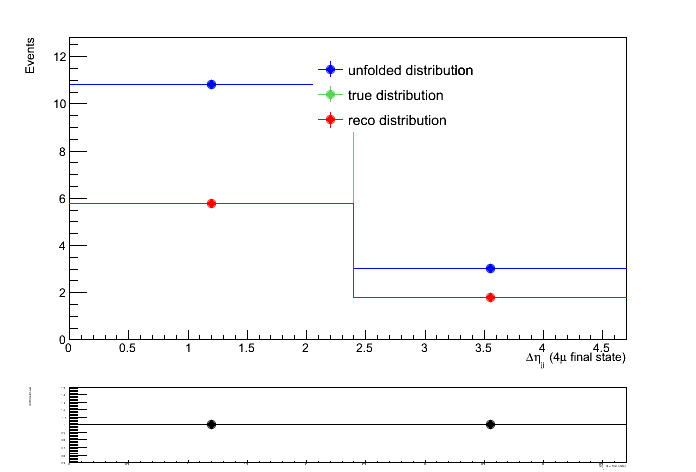
\includegraphics[width=\cmsFigWidth]{Figures/Unfolding/MCTests/Deta_ZZTo4m_MadMatrix_MadDistr_FullSample}
%%      \caption{Unfolding test: \texttt{MadGraph} matrix applied on \texttt{MadGraph} distribution, using the full set. Results are reported as a function of 
%%  the invariant mass of the 4-lepton system (top left), the number of jets in the event (top right), the invariant mass of the two most energetic jets (bottom left) and the $\Delta\eta$ between them (bottom right) for the $4\mu$ final state.}
%%     \label{fig:FullMad_4m}
%%   \end{center}
%% \end{figure}
%% \begin{figure}[hbtp]
%%   \begin{center}
%%     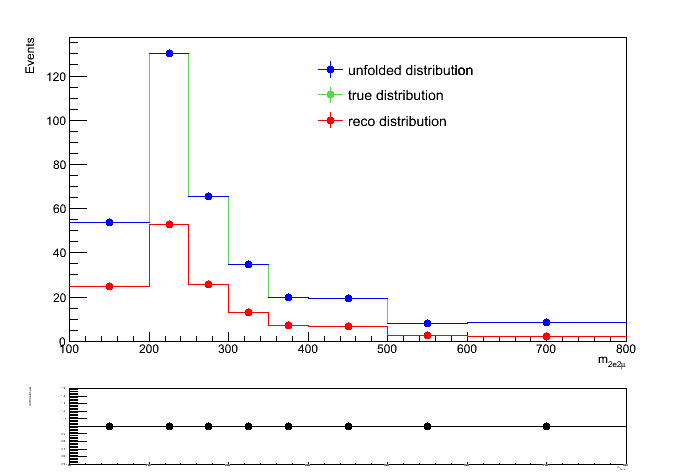
\includegraphics[width=\cmsFigWidth]{Figures/Unfolding/MCTests/Mass_ZZTo2e2m_MadMatrix_MadDistr_FullSample}     
%%     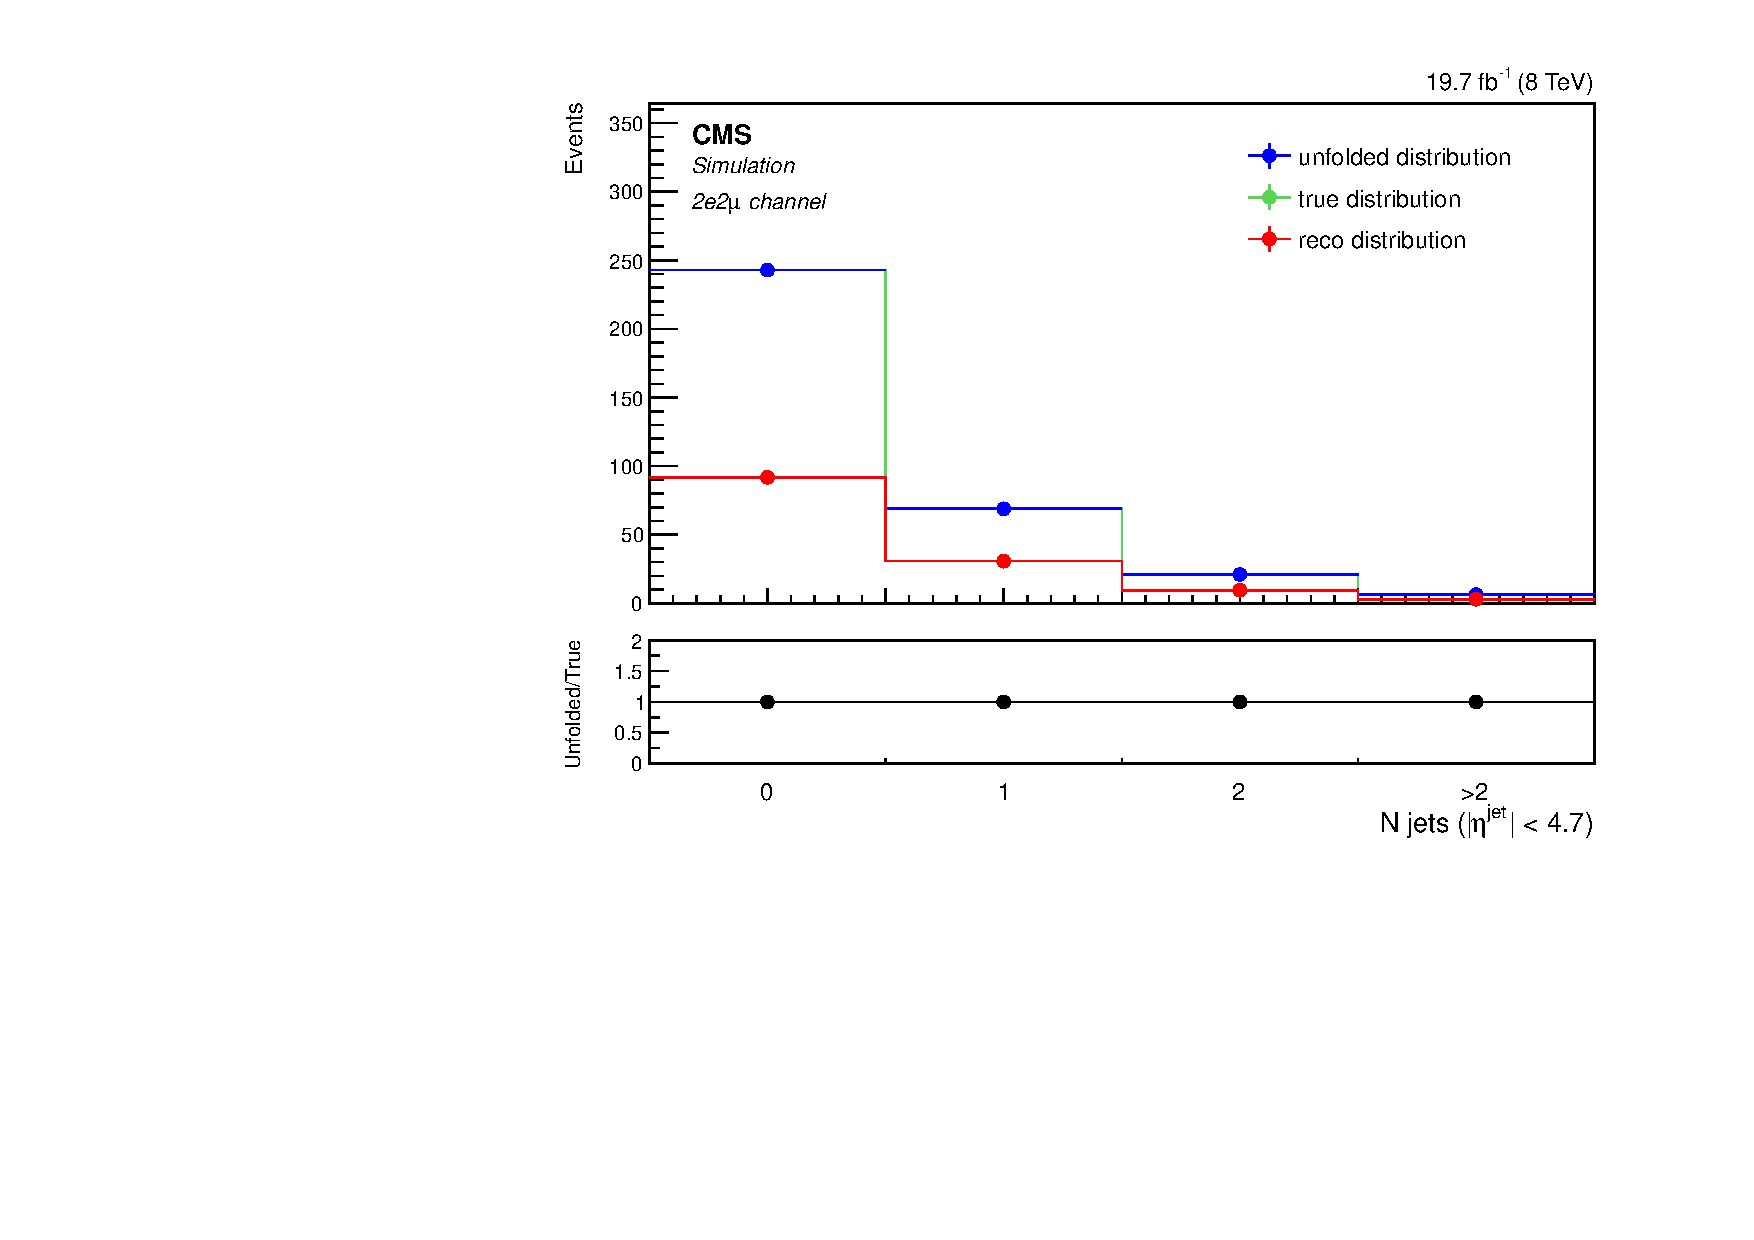
\includegraphics[width=\cmsFigWidth]{Figures/Unfolding/MCTests/Jets_ZZTo2e2m_MadMatrix_MadDistr_FullSample}
%%      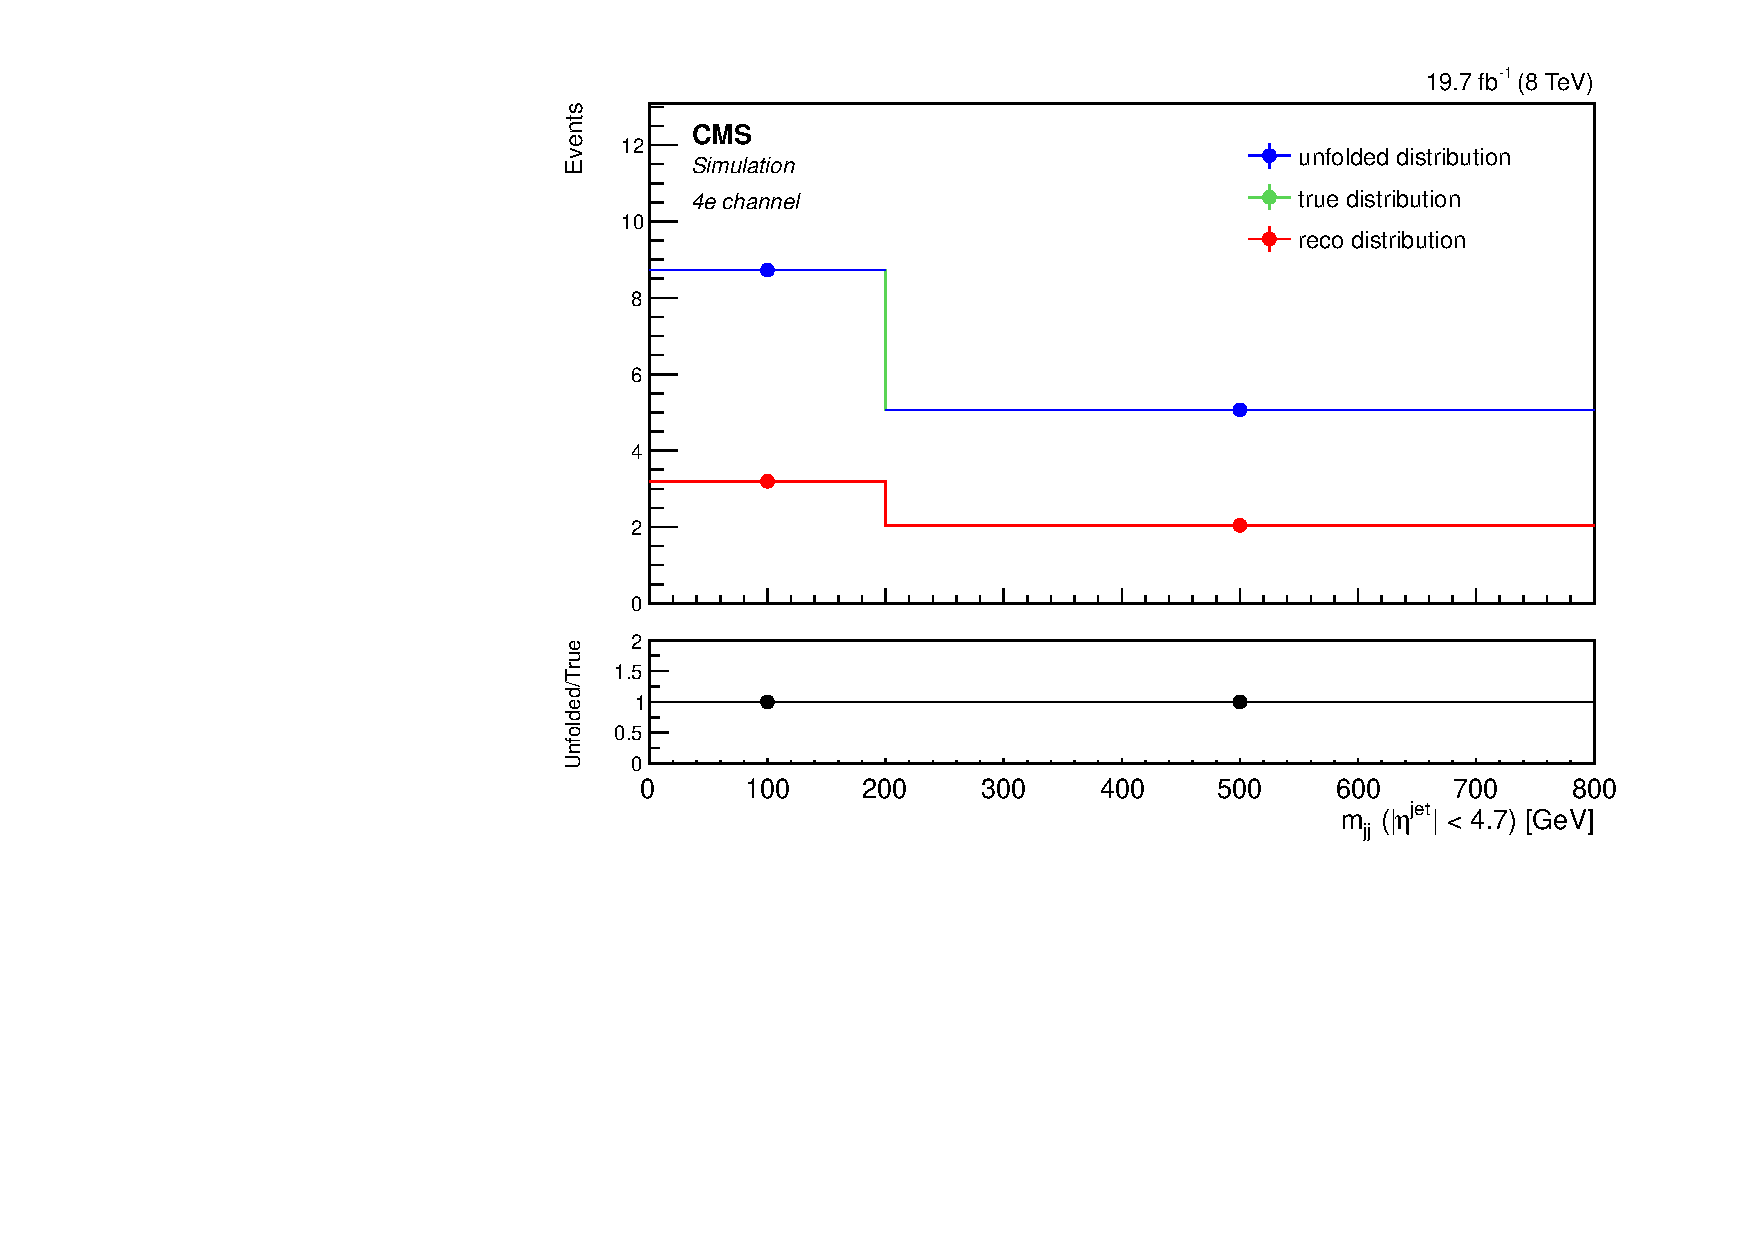
\includegraphics[width=\cmsFigWidth]{Figures/Unfolding/MCTests/Mjj_ZZTo4e_MadMatrix_MadDistr_FullSample}
%%      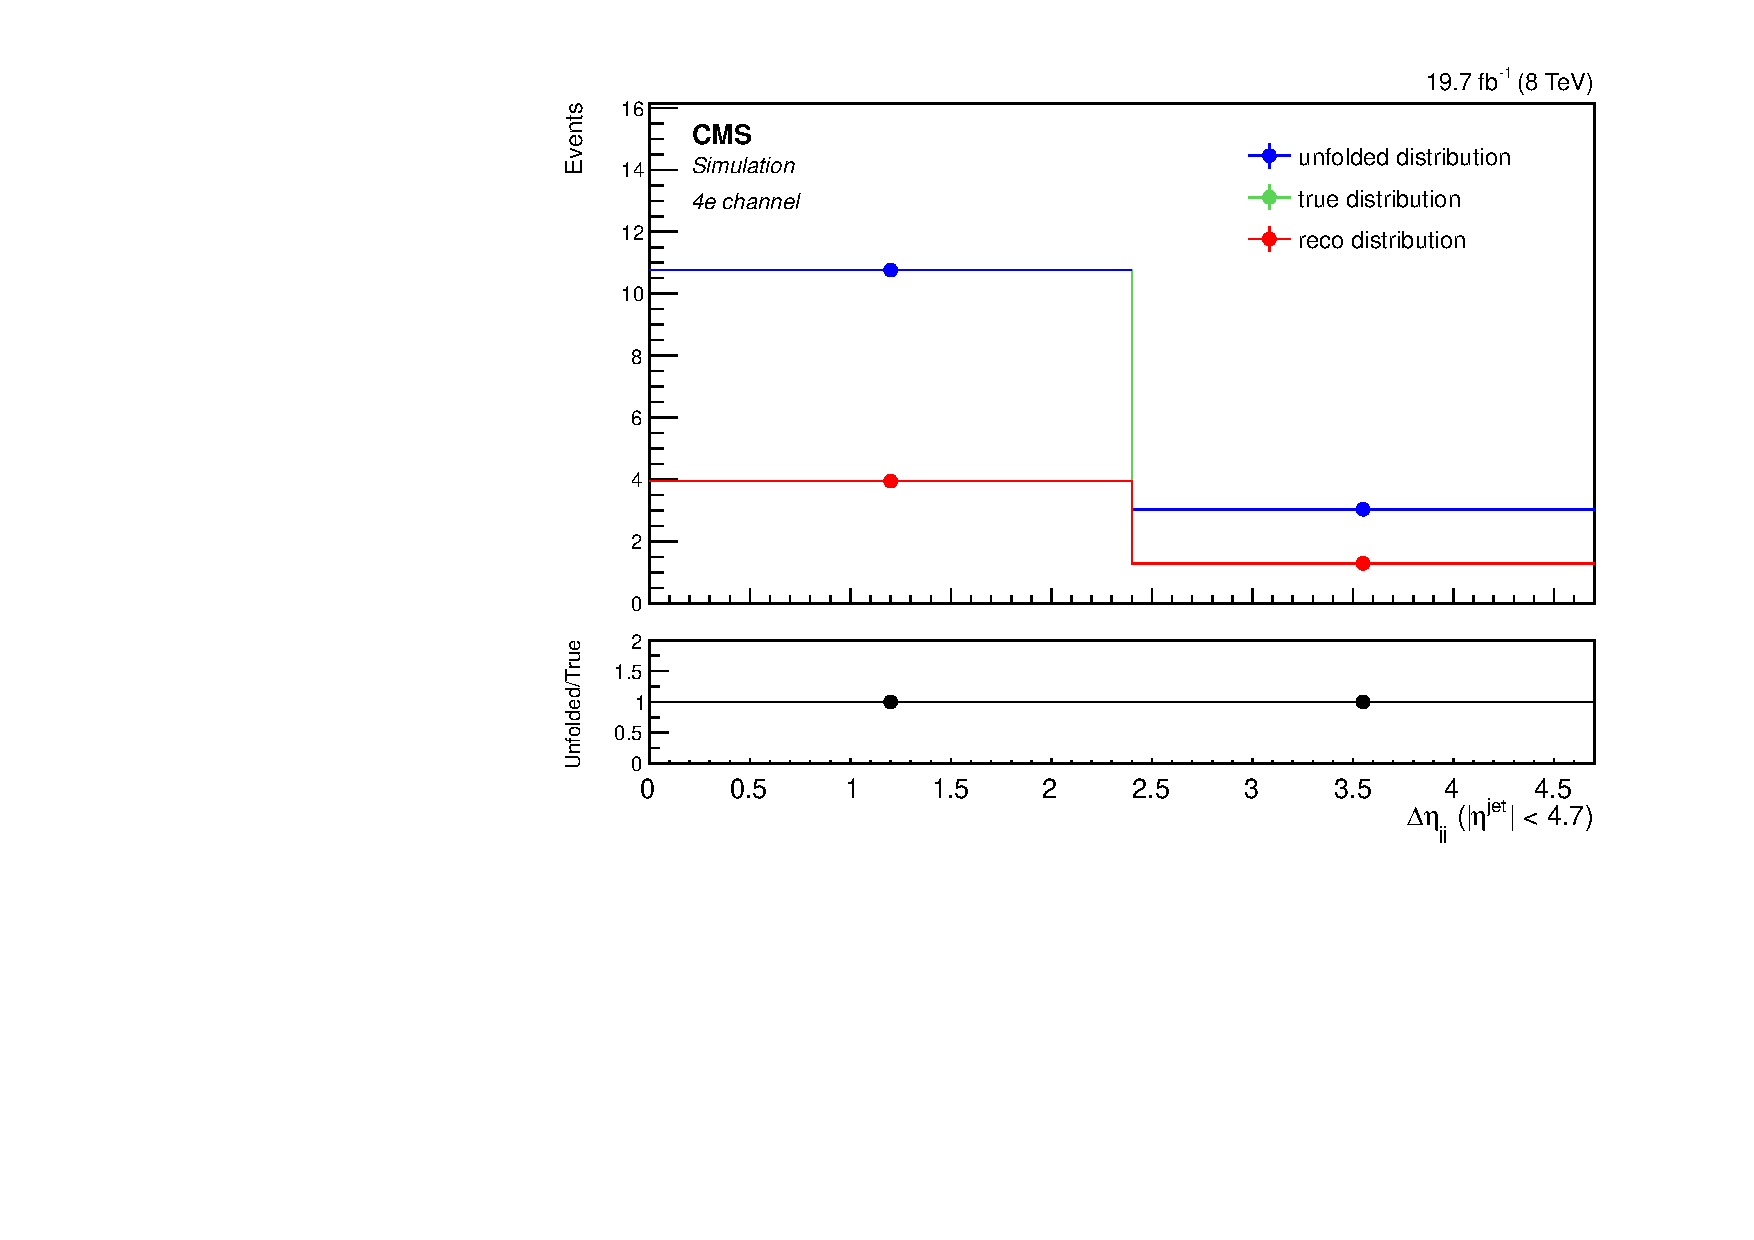
\includegraphics[width=\cmsFigWidth]{Figures/Unfolding/MCTests/Deta_ZZTo4e_MadMatrix_MadDistr_FullSample}
%%      \caption{Unfolding test: \texttt{MadGraph} matrix applied on \texttt{MadGraph} distribution, using the full set. Results are reported as a function of 
%%  the invariant mass of the 4-lepton system (top left), the number of jets in the event (top right), the invariant mass of the two most energetic jets (bottom left) and the $\Delta\eta$ between them (bottom right) for the $2e2\mu$ final state}
%%     \label{fig:FullMad_2e2m}
%%   \end{center}
%% \end{figure}
%% \begin{figure}[hbtp]
%%   \begin{center}
%%     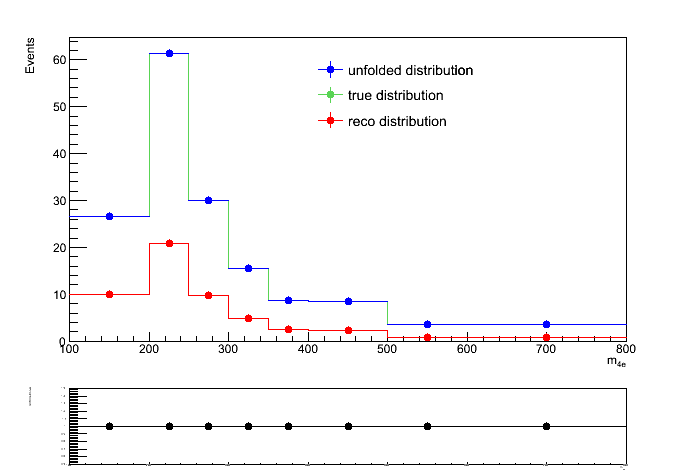
\includegraphics[width=\cmsFigWidth]{Figures/Unfolding/MCTests/Mass_ZZTo4e_PowMatrix_PowDistr_FullSample}     
%%     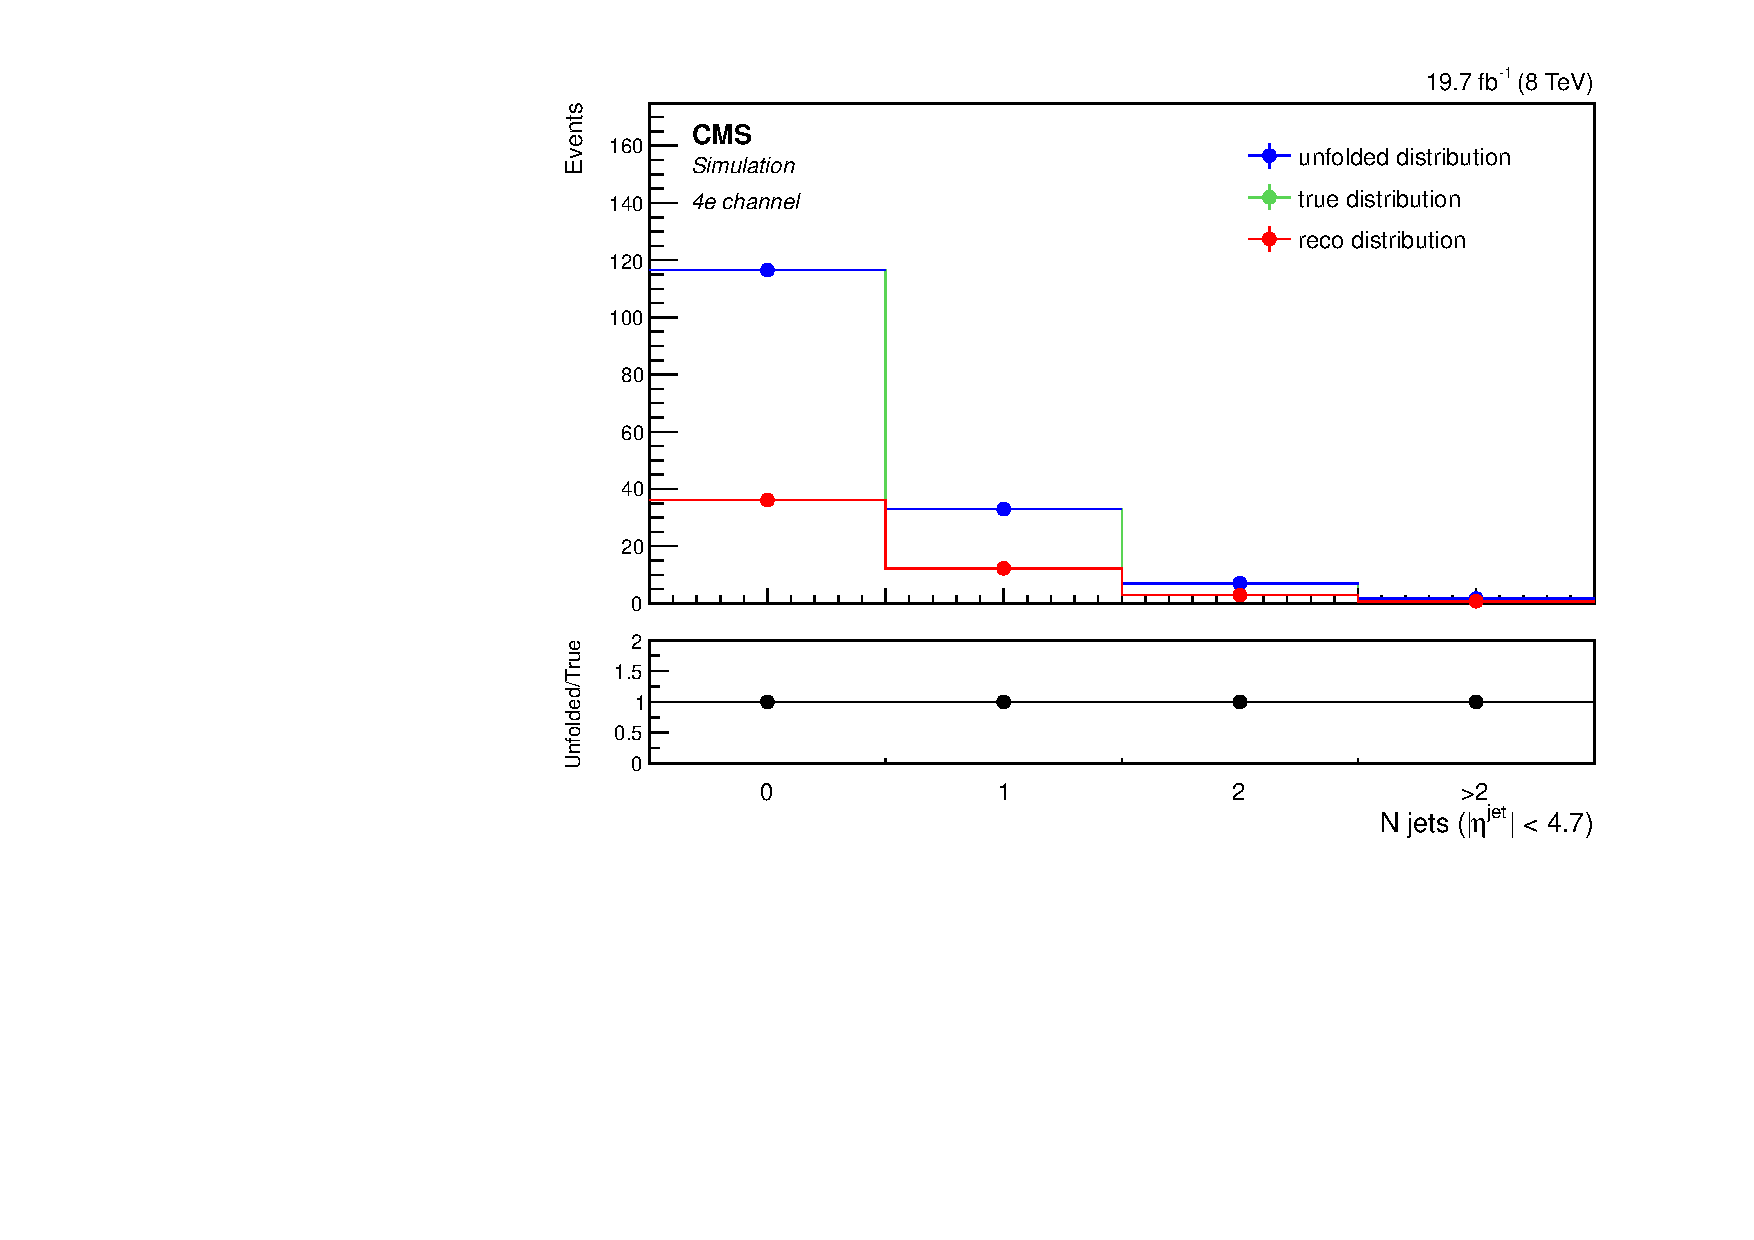
\includegraphics[width=\cmsFigWidth]{Figures/Unfolding/MCTests/Jets_ZZTo4e_PowMatrix_PowDistr_FullSample}
%%      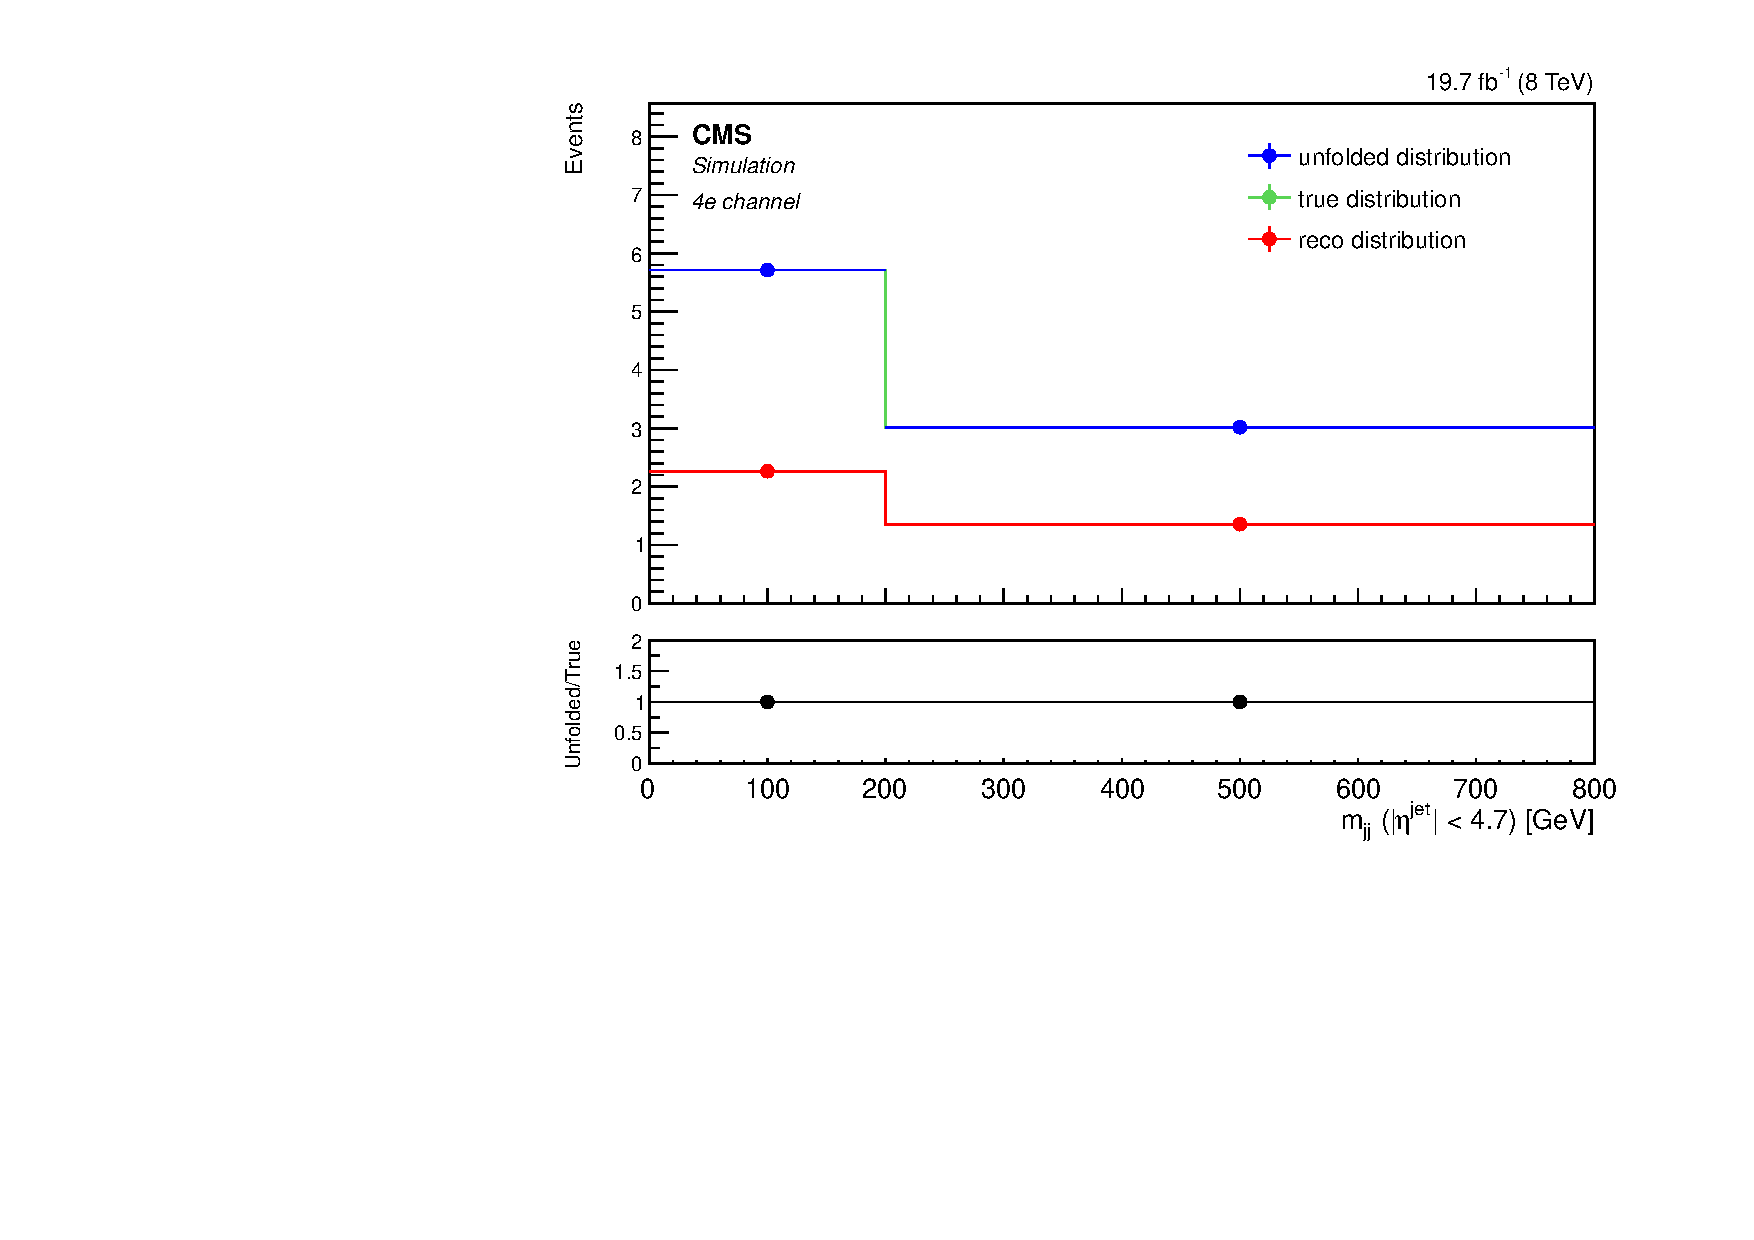
\includegraphics[width=\cmsFigWidth]{Figures/Unfolding/MCTests/Mjj_ZZTo4e_PowMatrix_PowDistr_FullSample}
%%      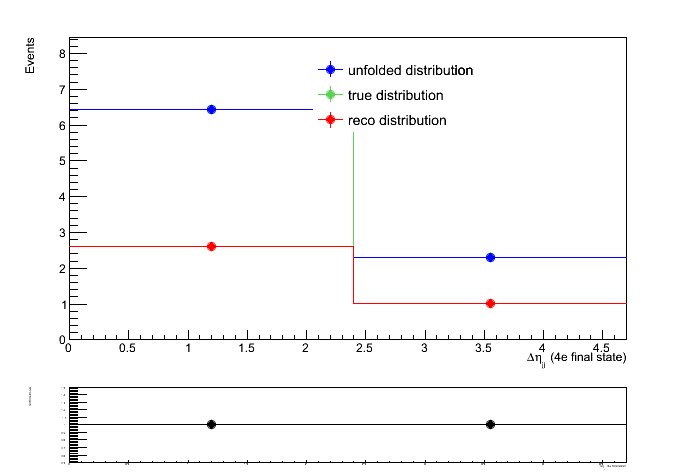
\includegraphics[width=\cmsFigWidth]{Figures/Unfolding/MCTests/Deta_ZZTo4e_PowMatrix_PowDistr_FullSample}
%%      \caption{Unfolding test: \texttt{Powheg} matrix applied on \texttt{Powheg} distribution, using the full set. Results are reported as a function of 
%%  the invariant mass of the 4-lepton system (top left), the number of jets in the event (top right), the invariant mass of the two most energetic jets (bottom left) and the $\Delta\eta$ between them (bottom right) for the $4e$ final state.}
%%     \label{fig:FullPow_4e}
%%   \end{center}
%% \end{figure}
%% \begin{figure}[hbtp]
%%   \begin{center}
%%     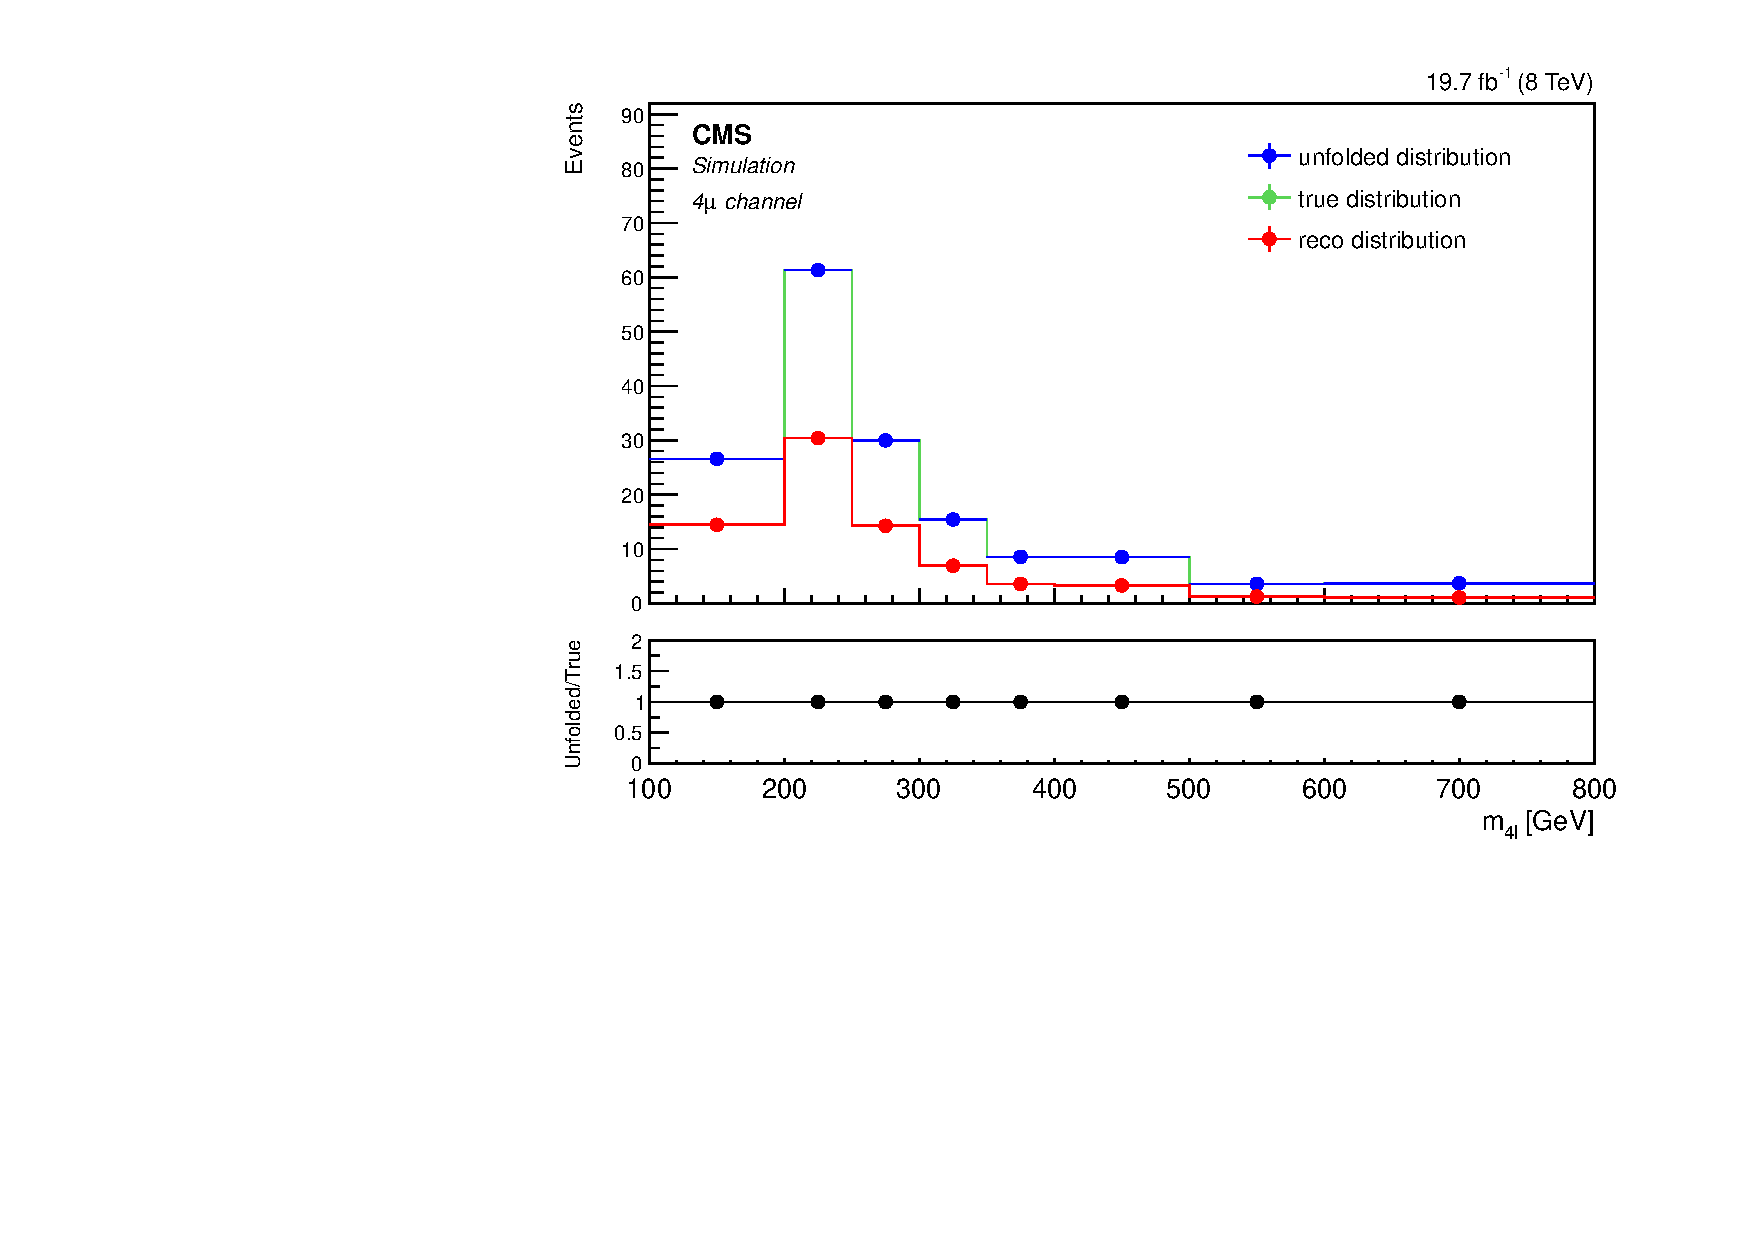
\includegraphics[width=\cmsFigWidth]{Figures/Unfolding/MCTests/Mass_ZZTo4m_PowMatrix_PowDistr_FullSample}     
%%     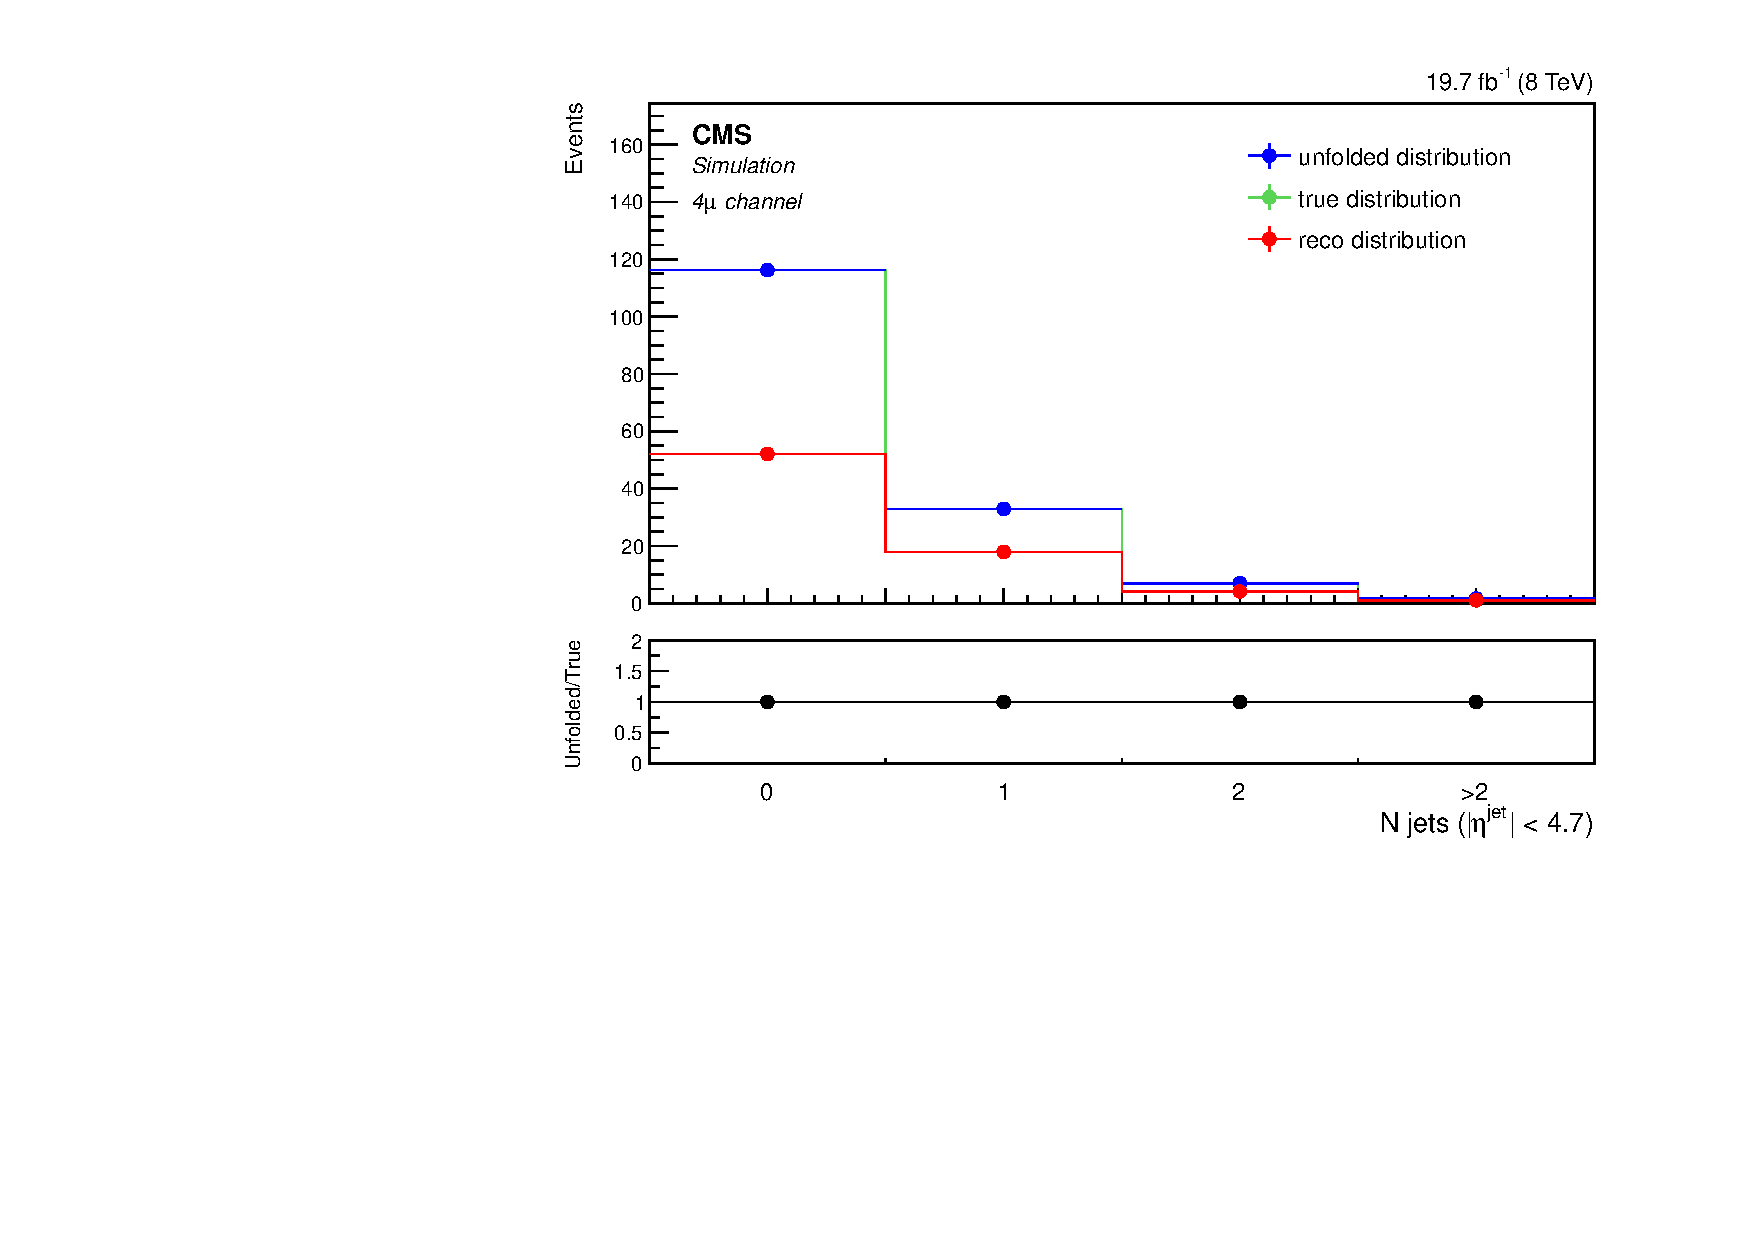
\includegraphics[width=\cmsFigWidth]{Figures/Unfolding/MCTests/Jets_ZZTo4m_PowMatrix_PowDistr_FullSample}
%%      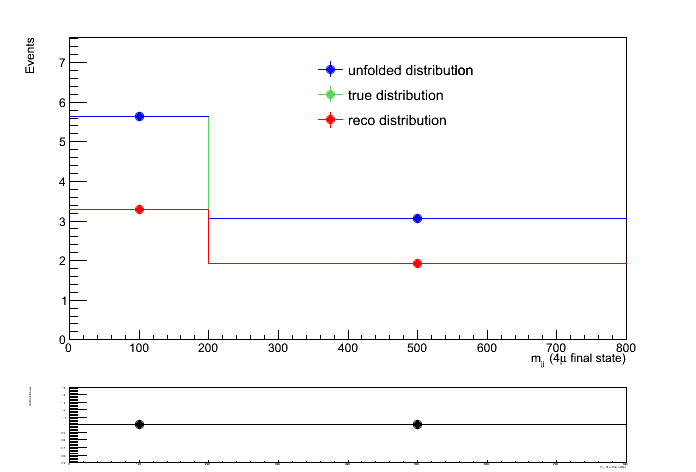
\includegraphics[width=\cmsFigWidth]{Figures/Unfolding/MCTests/Mjj_ZZTo4m_PowMatrix_PowDistr_FullSample}
%%      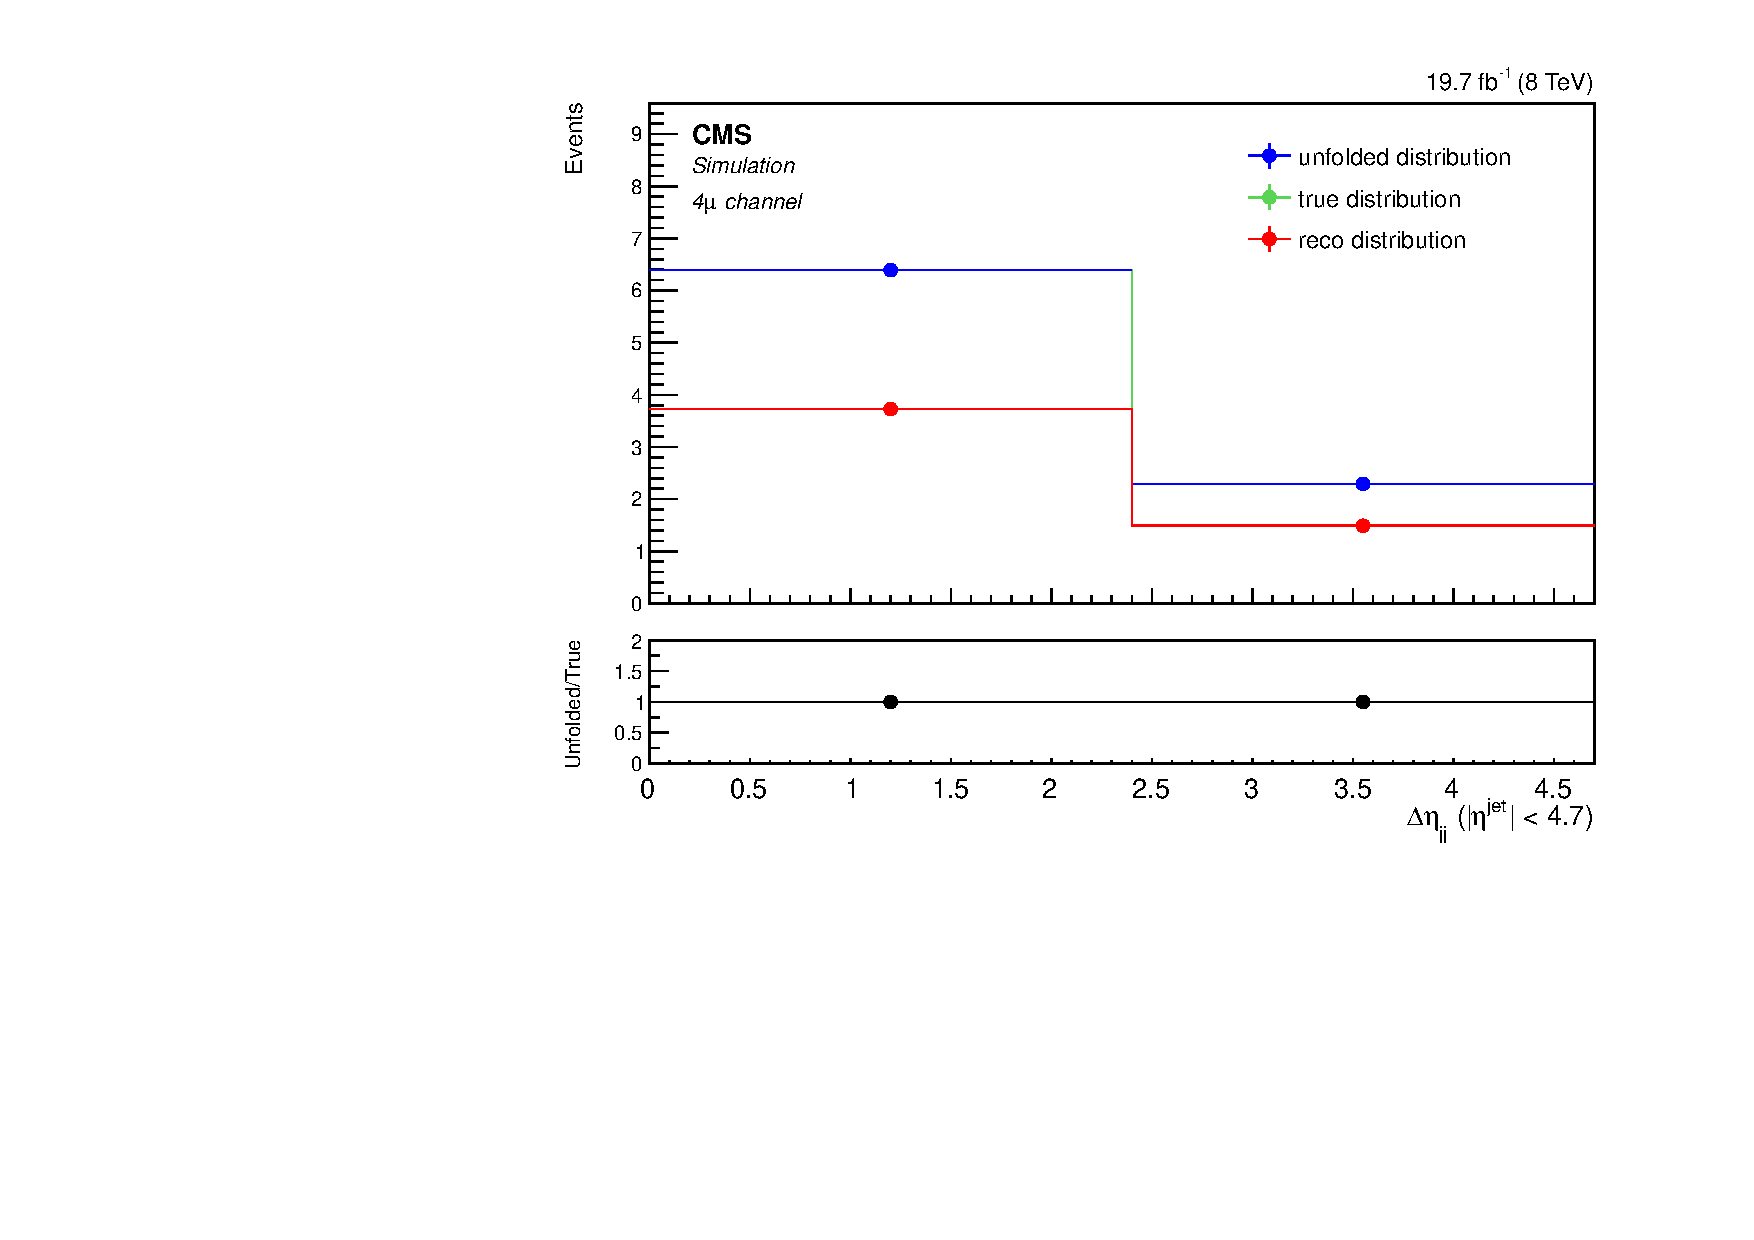
\includegraphics[width=\cmsFigWidth]{Figures/Unfolding/MCTests/Deta_ZZTo4m_PowMatrix_PowDistr_FullSample}
%%      \caption{Unfolding test: \texttt{Powheg} matrix applied on \texttt{Powheg} distribution, using the full set. Results are reported as a function of 
%%  the invariant mass of the 4-lepton system (top left), the number of jets in the event (top right), the invariant mass of the two most energetic jets (bottom left) and the $\Delta\eta$ between them (bottom right) for the $4\mu$ final state.}
%%     \label{fig:FullPow_4m}
%%   \end{center}
%% \end{figure}
%% \begin{figure}[hbtp]
%%   \begin{center}
%%     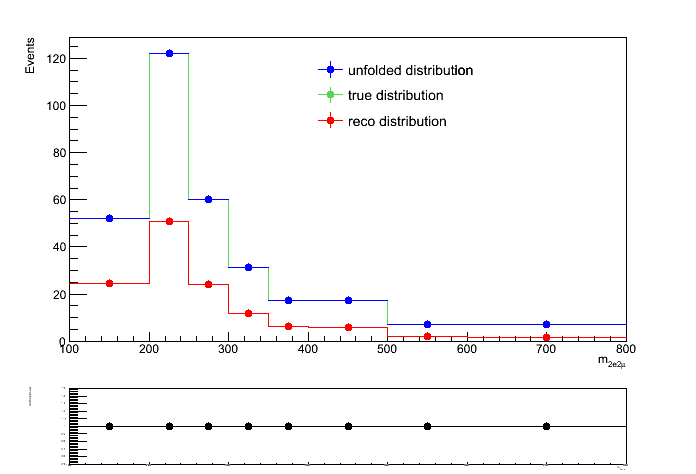
\includegraphics[width=\cmsFigWidth]{Figures/Unfolding/MCTests/Mass_ZZTo2e2m_PowMatrix_PowDistr_FullSample}     
%%     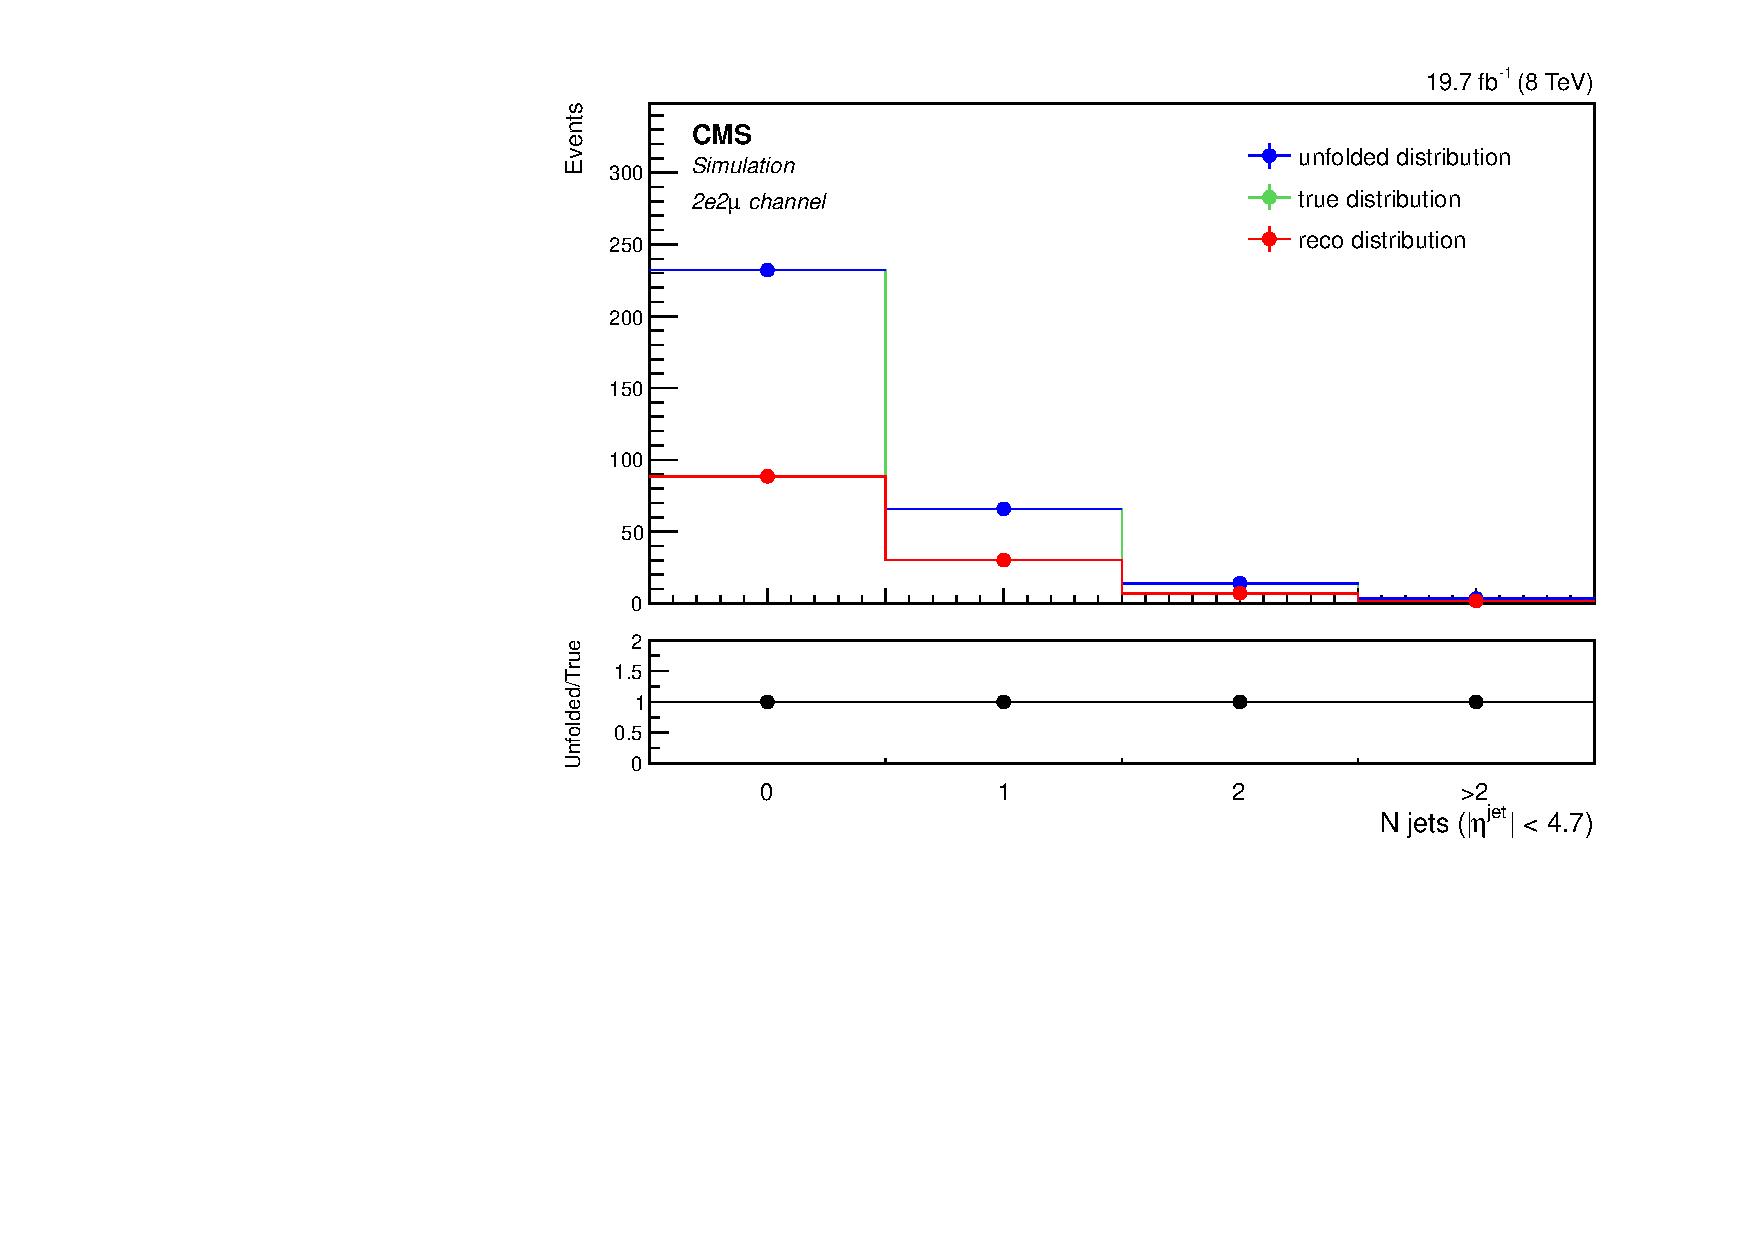
\includegraphics[width=\cmsFigWidth]{Figures/Unfolding/MCTests/Jets_ZZTo2e2m_PowMatrix_PowDistr_FullSample}
%%      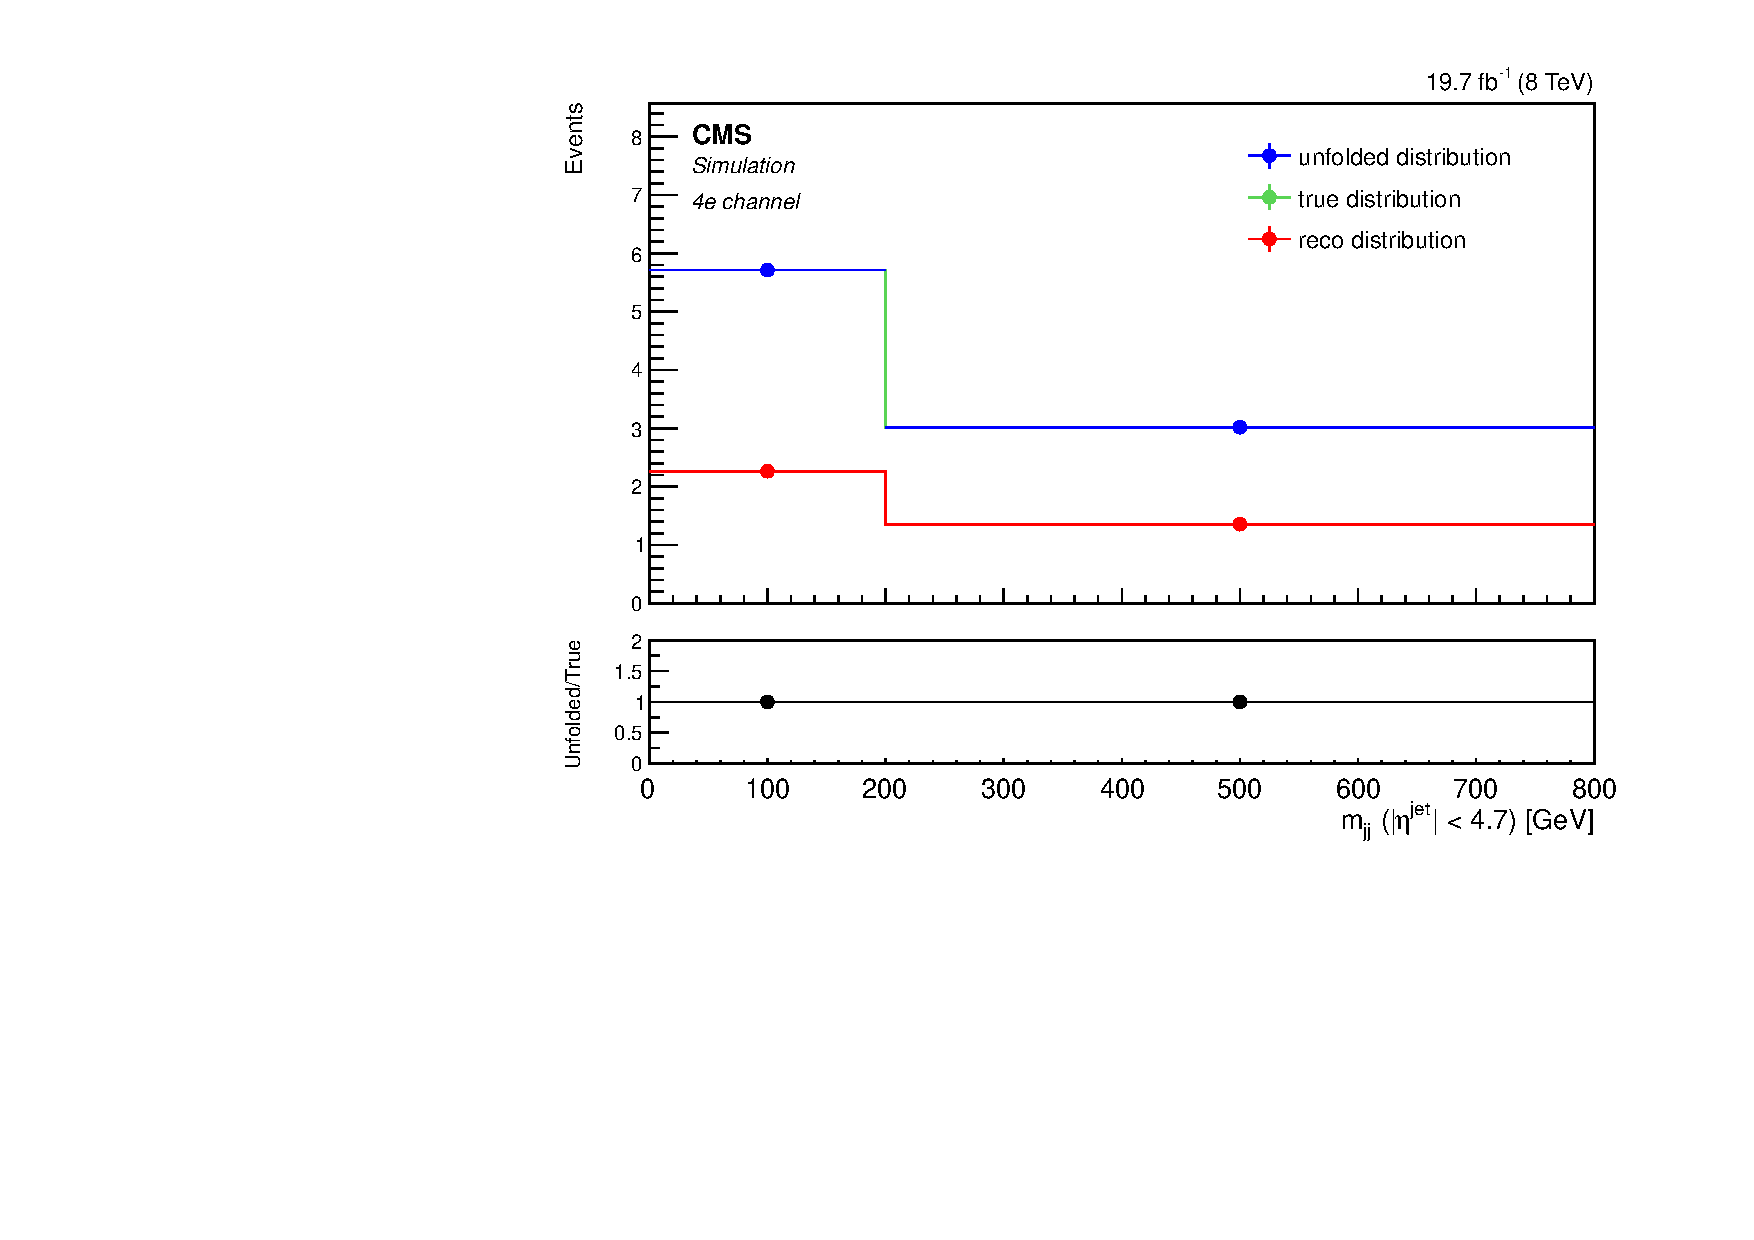
\includegraphics[width=\cmsFigWidth]{Figures/Unfolding/MCTests/Mjj_ZZTo4e_PowMatrix_PowDistr_FullSample}
%%      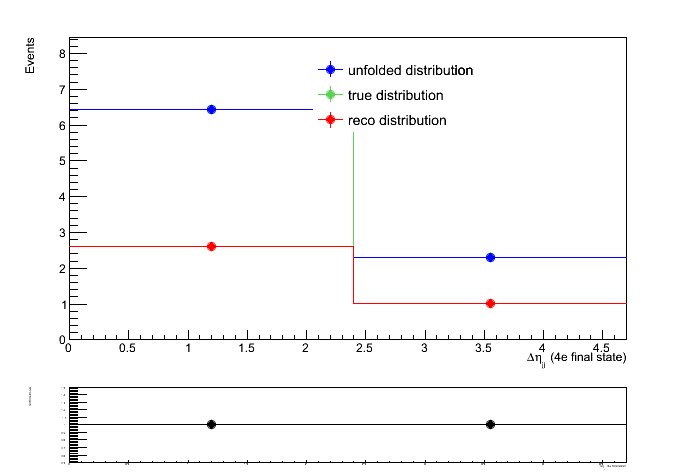
\includegraphics[width=\cmsFigWidth]{Figures/Unfolding/MCTests/Deta_ZZTo4e_PowMatrix_PowDistr_FullSample}
%%      \caption{Unfolding test: \texttt{Powheg} matrix applied on \texttt{Powheg} distribution, using the full set. Results are reported as a function of 
%%  the invariant mass of the 4-lepton system (top left), the number of jets in the event (top right), the invariant mass of the two most energetic jets (bottom left) and the $\Delta\eta$ between them (bottom right) for the $2e2\mu$ final state}
%%     \label{fig:FullPow_2e2m}
%%   \end{center}
%% \end{figure}
%% \begin{figure}[hbtp]
%%   \begin{center}
%%     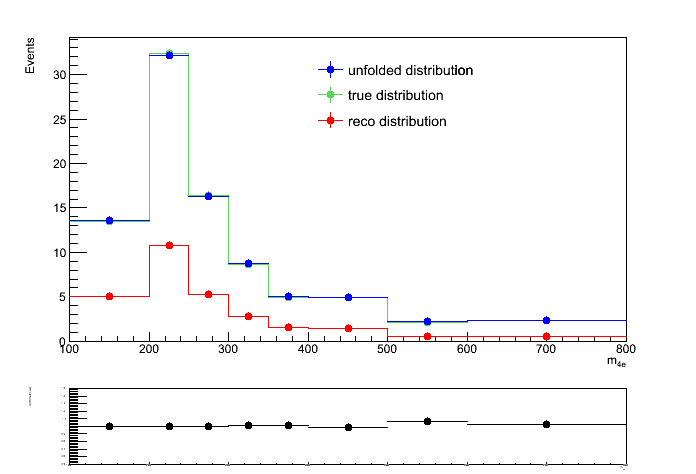
\includegraphics[width=\cmsFigWidth]{Figures/Unfolding/MCTests/Mass_ZZTo4e_MadMatrix_MadDistr_HalfSample}     
%%     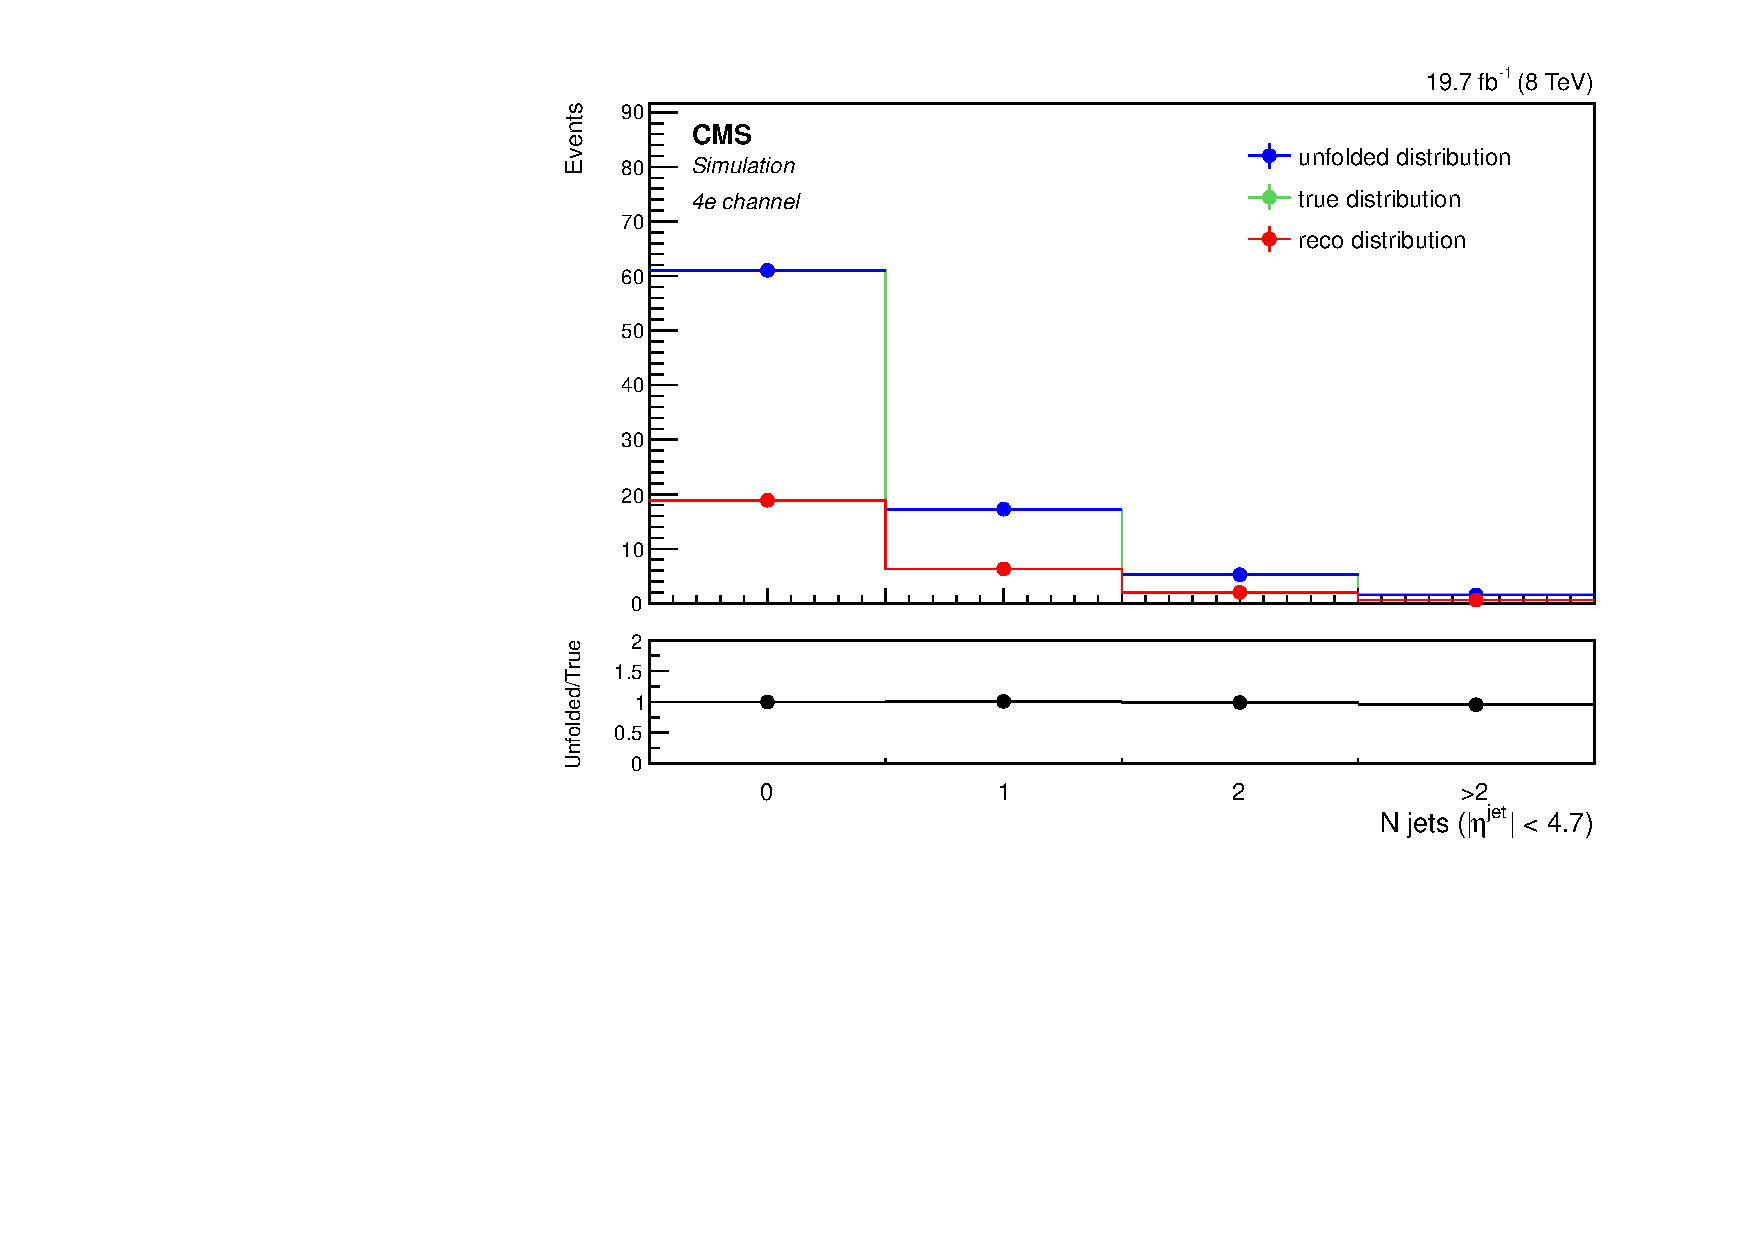
\includegraphics[width=\cmsFigWidth]{Figures/Unfolding/MCTests/Jets_ZZTo4e_MadMatrix_MadDistr_HalfSample}
%%      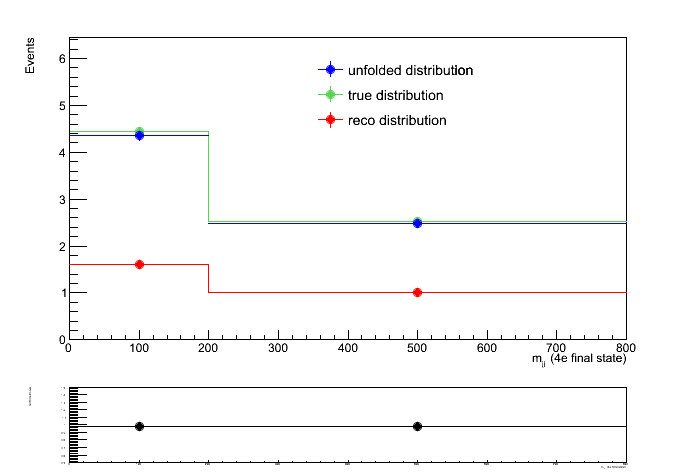
\includegraphics[width=\cmsFigWidth]{Figures/Unfolding/MCTests/Mjj_ZZTo4e_MadMatrix_MadDistr_HalfSample}
%%      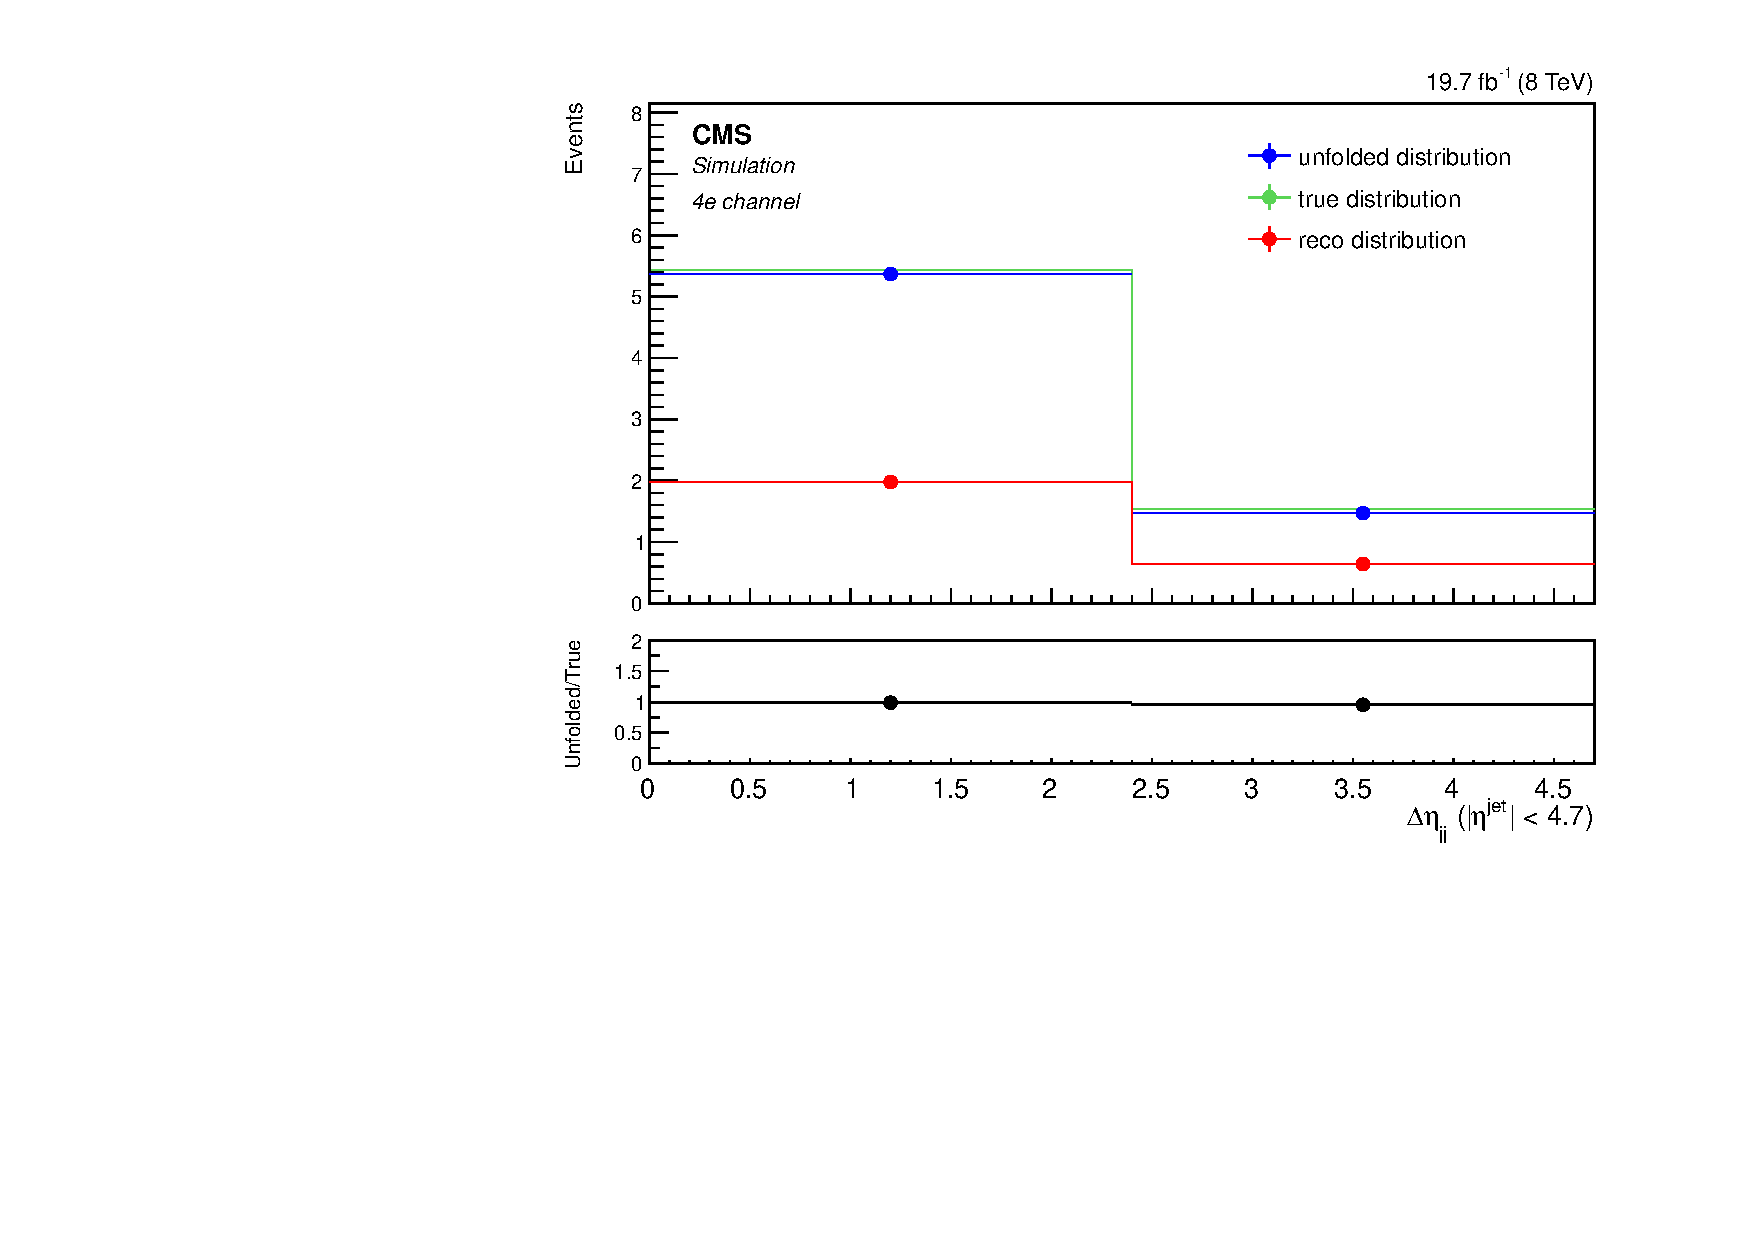
\includegraphics[width=\cmsFigWidth]{Figures/Unfolding/MCTests/Deta_ZZTo4e_MadMatrix_MadDistr_HalfSample}
%%      \caption{Unfolding test: \texttt{MadGraph} matrix applied on \texttt{MadGraph} distribution, using the two different halfs of the total sample. 
%%      Results are reported as a function of the invariant mass of the 4-lepton system (top left), the number of jets in the event (top right), the invariant mass of the
%%       two most energetic jets (bottom left) and the $\Delta\eta$ between them (bottom right) for the $4e$ final state.}
%%     \label{fig:HalfMad_4e}
%%   \end{center}
%% \end{figure}
%% \begin{figure}[hbtp]
%%   \begin{center}
%%     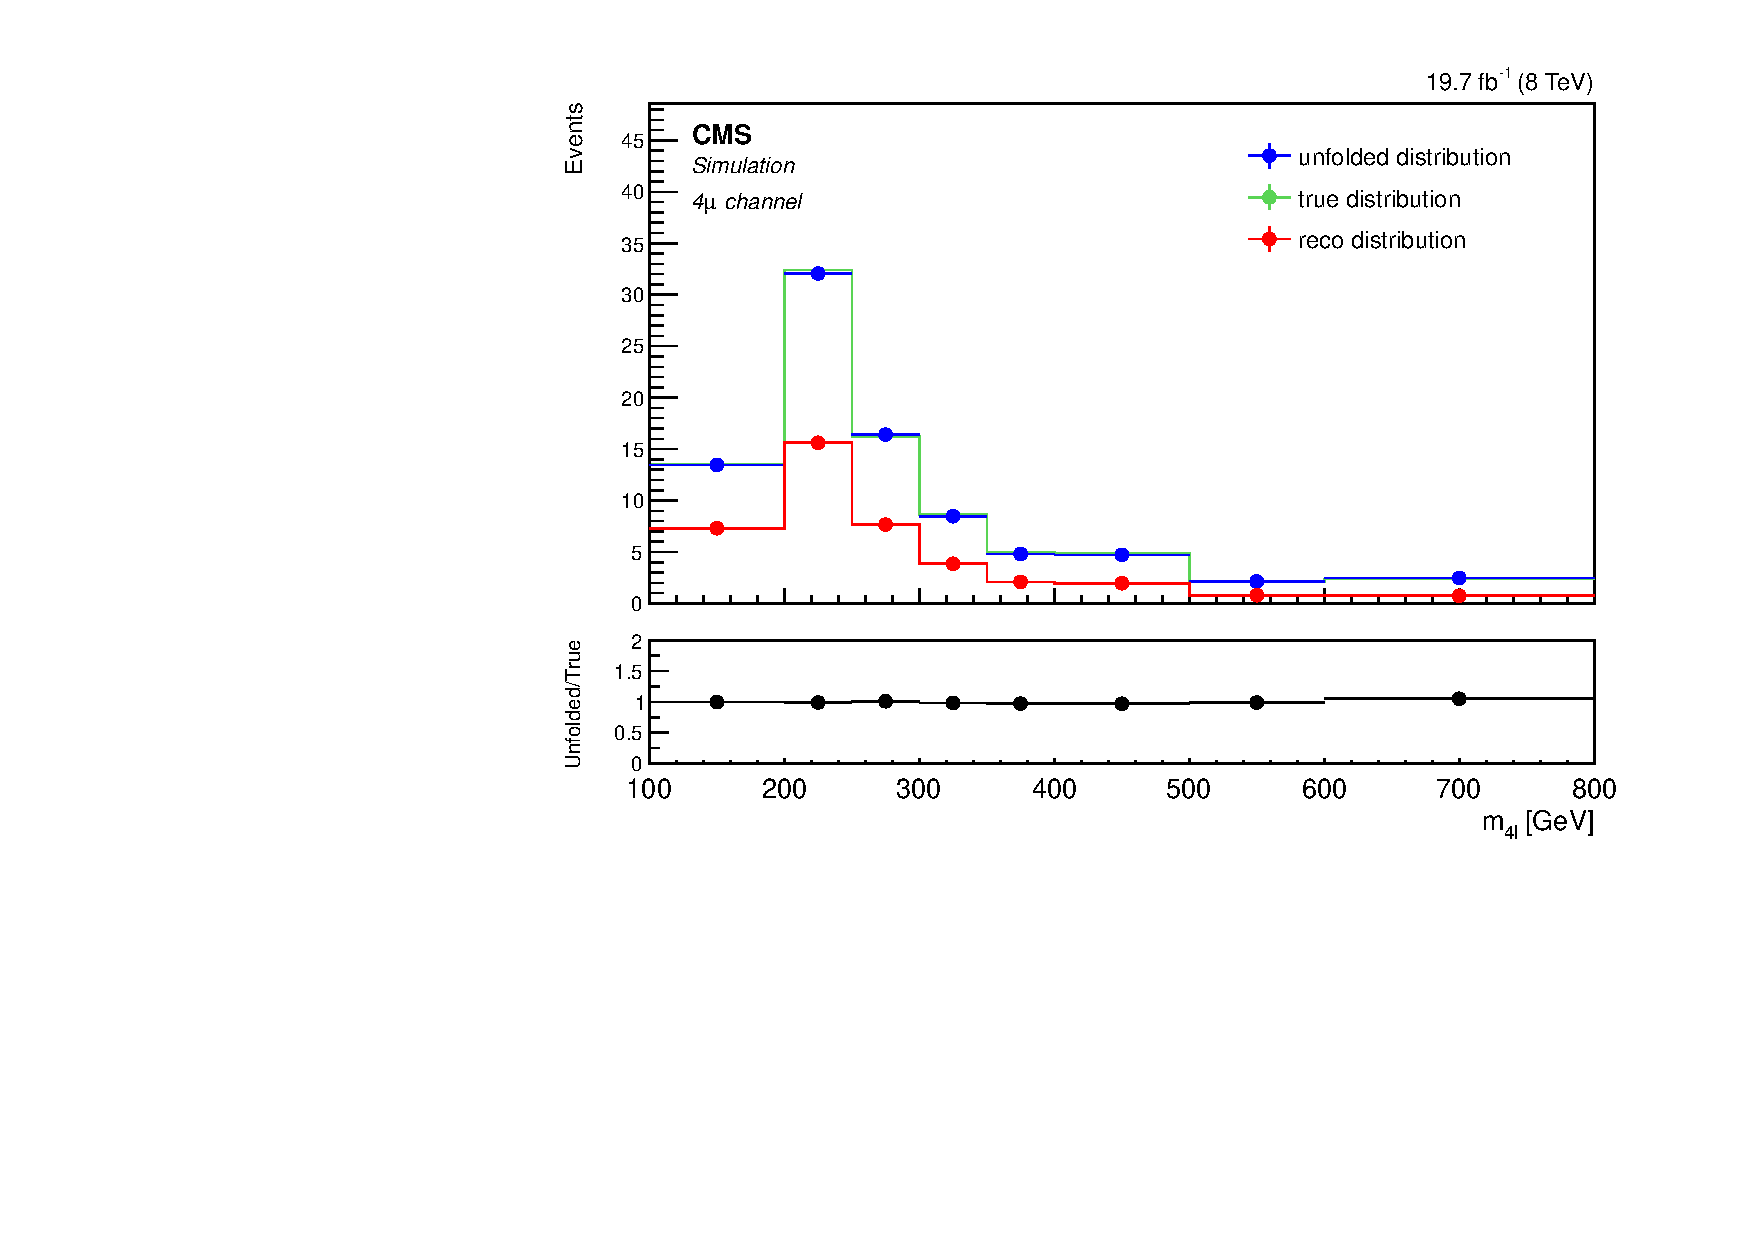
\includegraphics[width=\cmsFigWidth]{Figures/Unfolding/MCTests/Mass_ZZTo4m_MadMatrix_MadDistr_HalfSample}     
%%     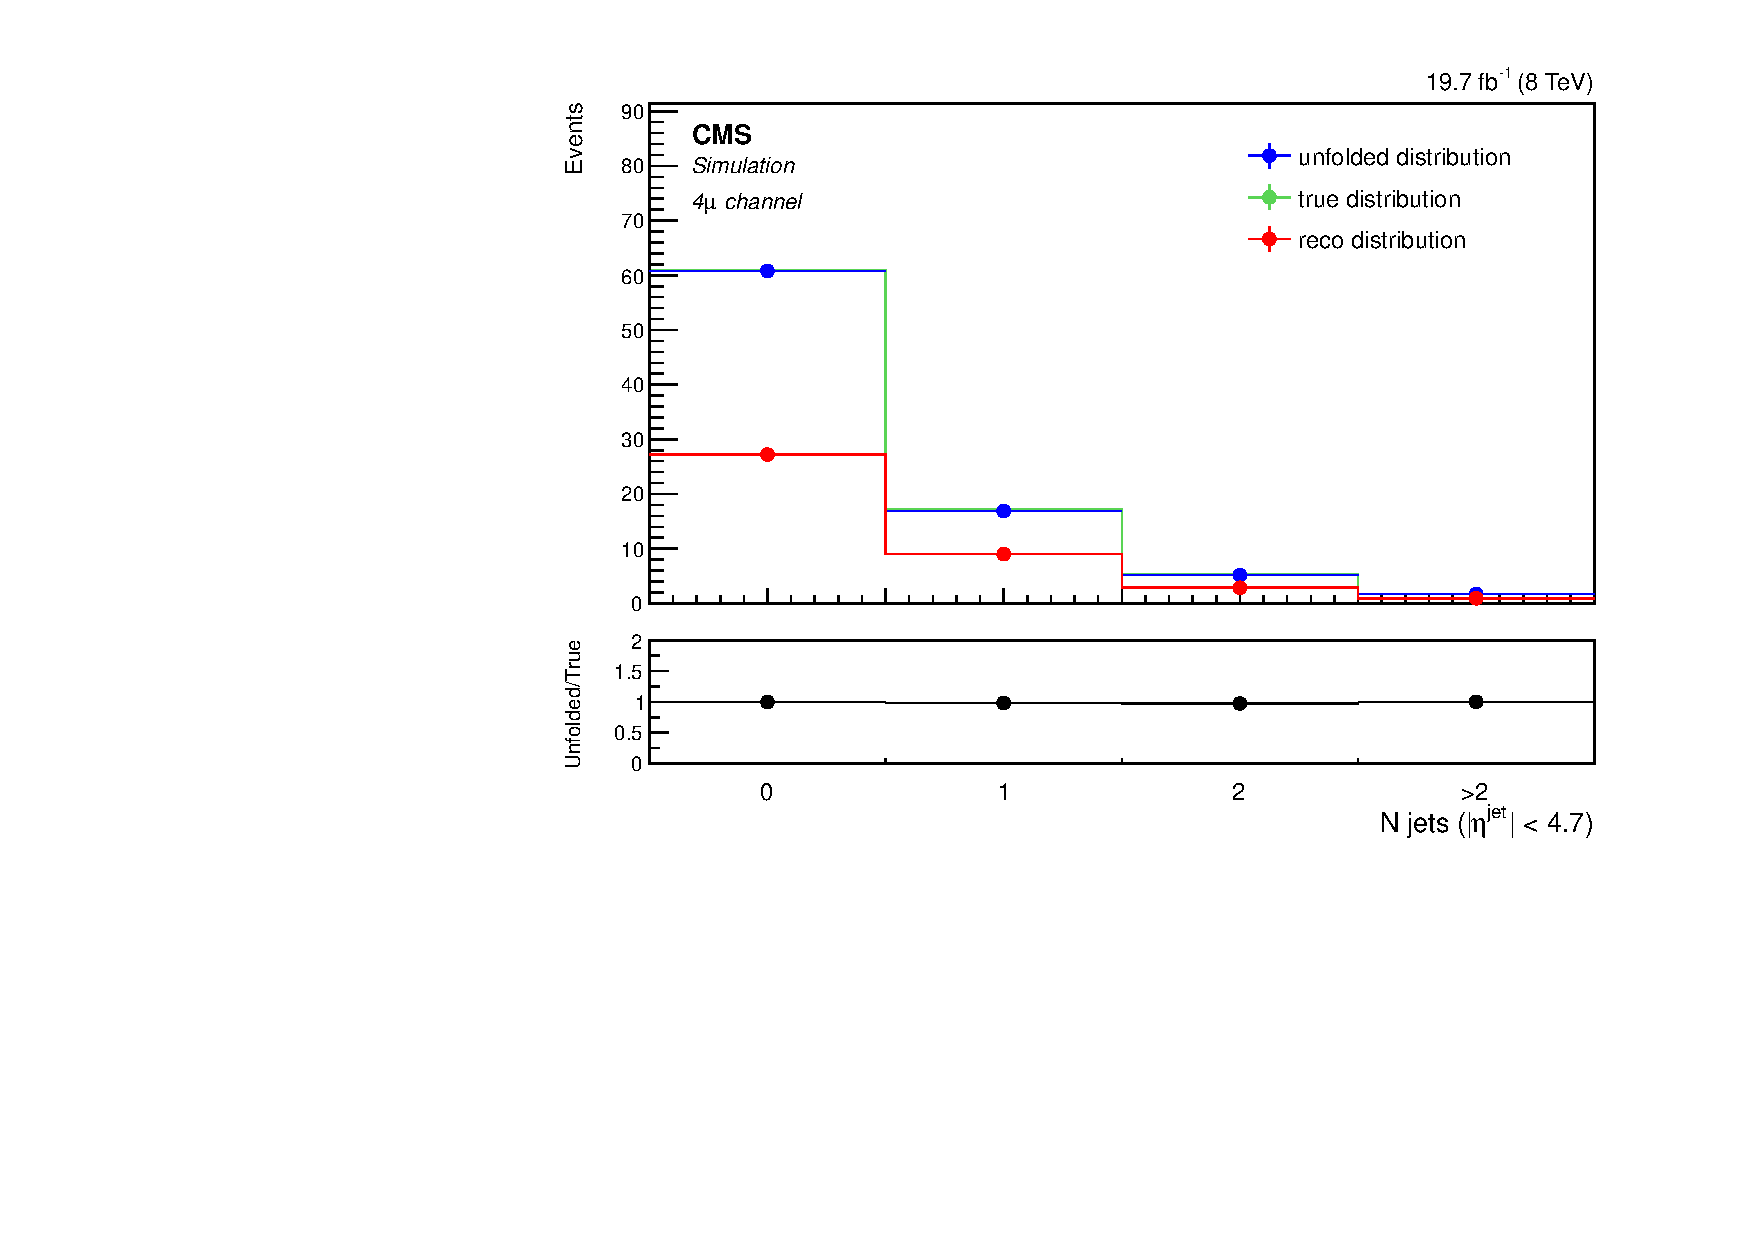
\includegraphics[width=\cmsFigWidth]{Figures/Unfolding/MCTests/Jets_ZZTo4m_MadMatrix_MadDistr_HalfSample}
%%      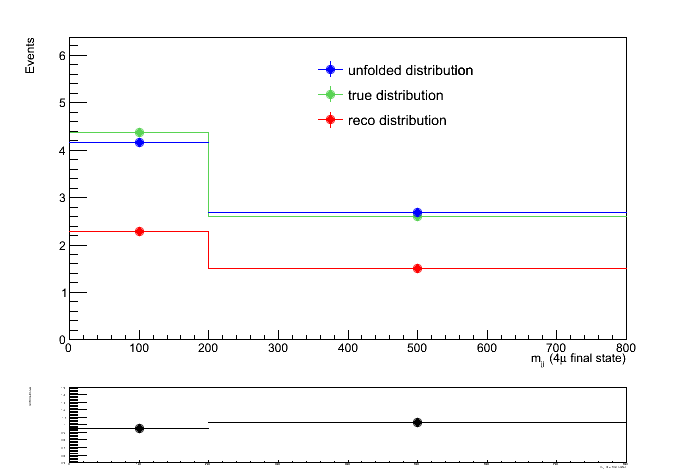
\includegraphics[width=\cmsFigWidth]{Figures/Unfolding/MCTests/Mjj_ZZTo4m_MadMatrix_MadDistr_HalfSample}
%%      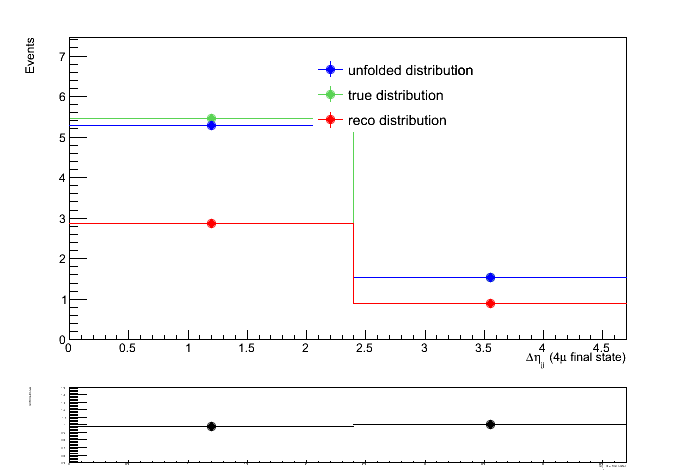
\includegraphics[width=\cmsFigWidth]{Figures/Unfolding/MCTests/Deta_ZZTo4m_MadMatrix_MadDistr_HalfSample}
%%      \caption{Unfolding test: \texttt{MadGraph} matrix applied on \texttt{MadGraph} distribution, using the two different halfs of the total sample. 
%%      Results are reported as a function of the invariant mass of the 4-lepton system (top left), the number of jets in the event (top right), the invariant mass of the
%%       two most energetic jets (bottom left) and the $\Delta\eta$ between them (bottom right) for the $4\mu$ final state.}
%%     \label{fig:HalfMad_4m}
%%      \end{center}
%% \end{figure}
%% \begin{figure}[hbtp]
%%   \begin{center}
%%     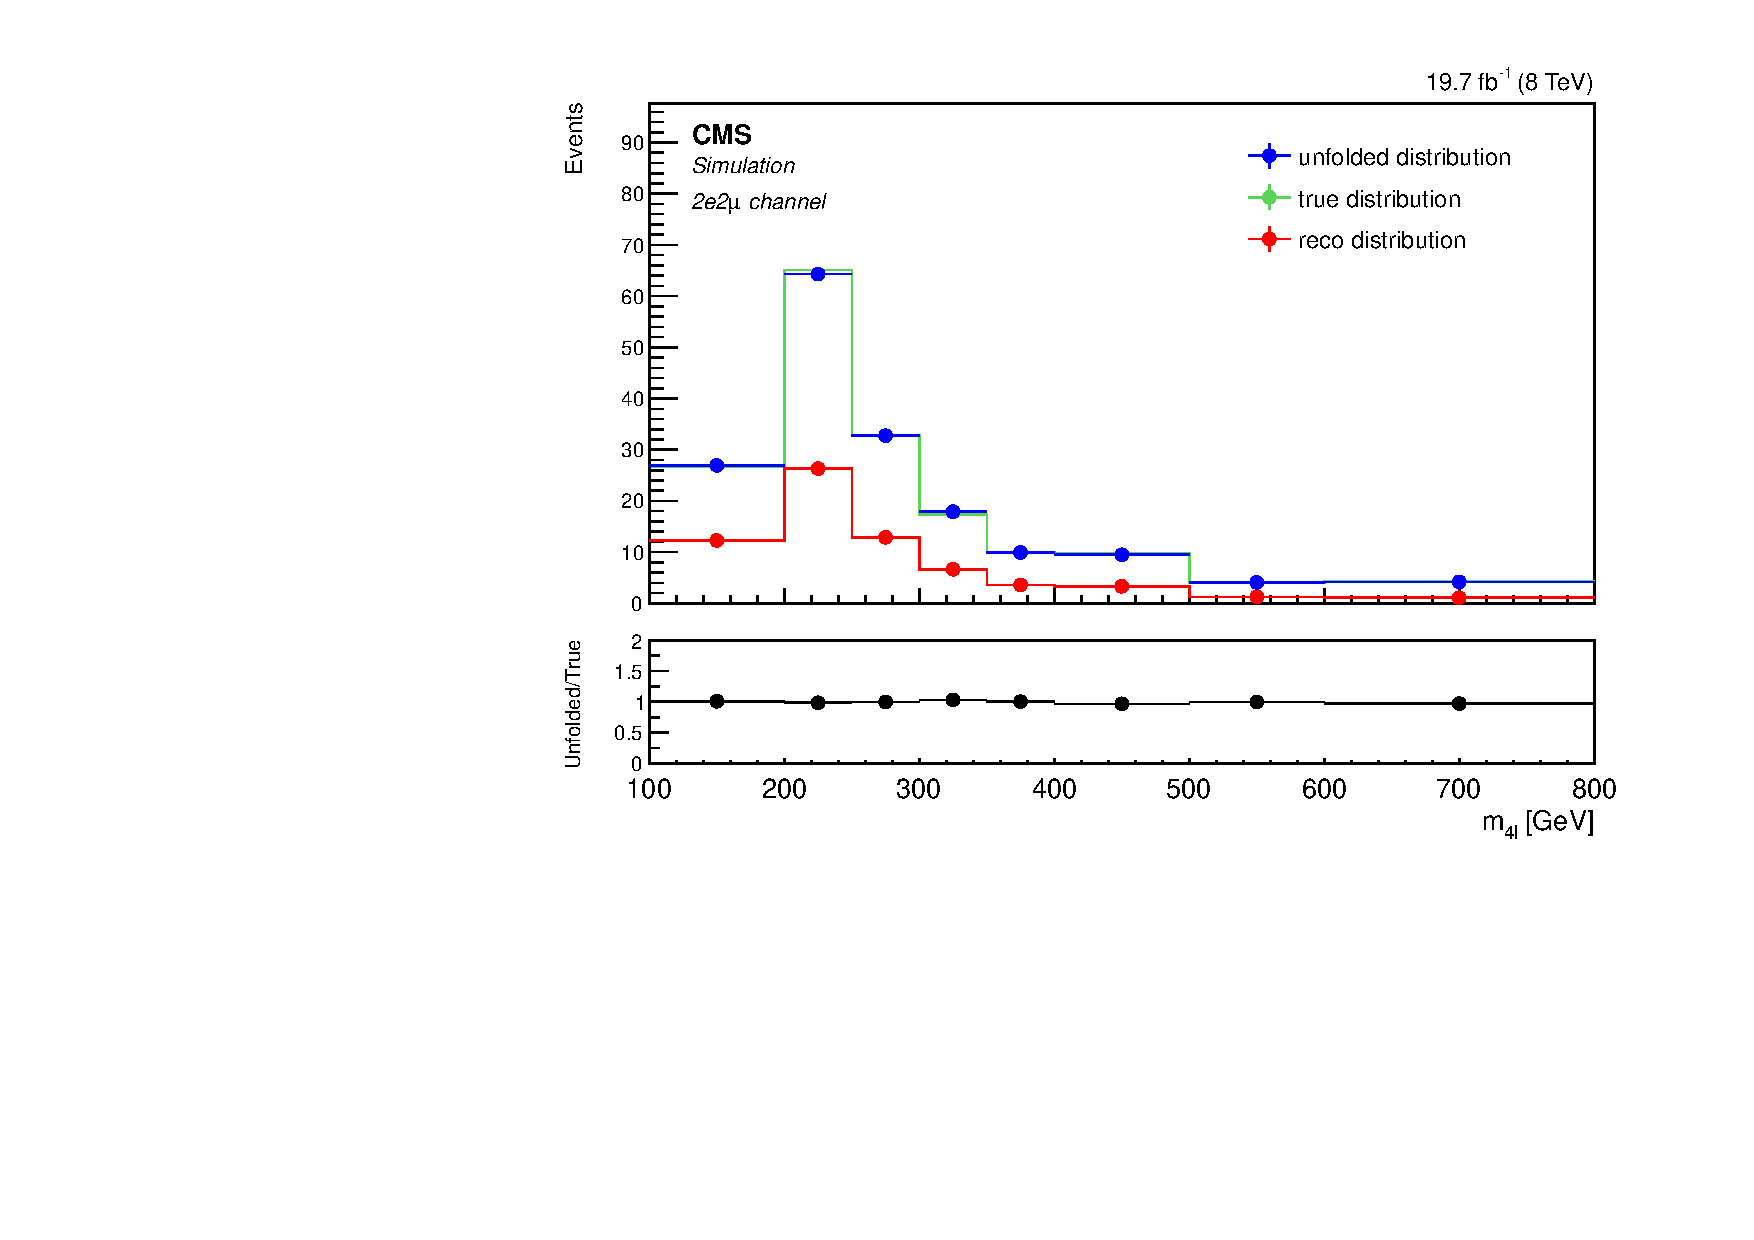
\includegraphics[width=\cmsFigWidth]{Figures/Unfolding/MCTests/Mass_ZZTo2e2m_MadMatrix_MadDistr_HalfSample}     
%%     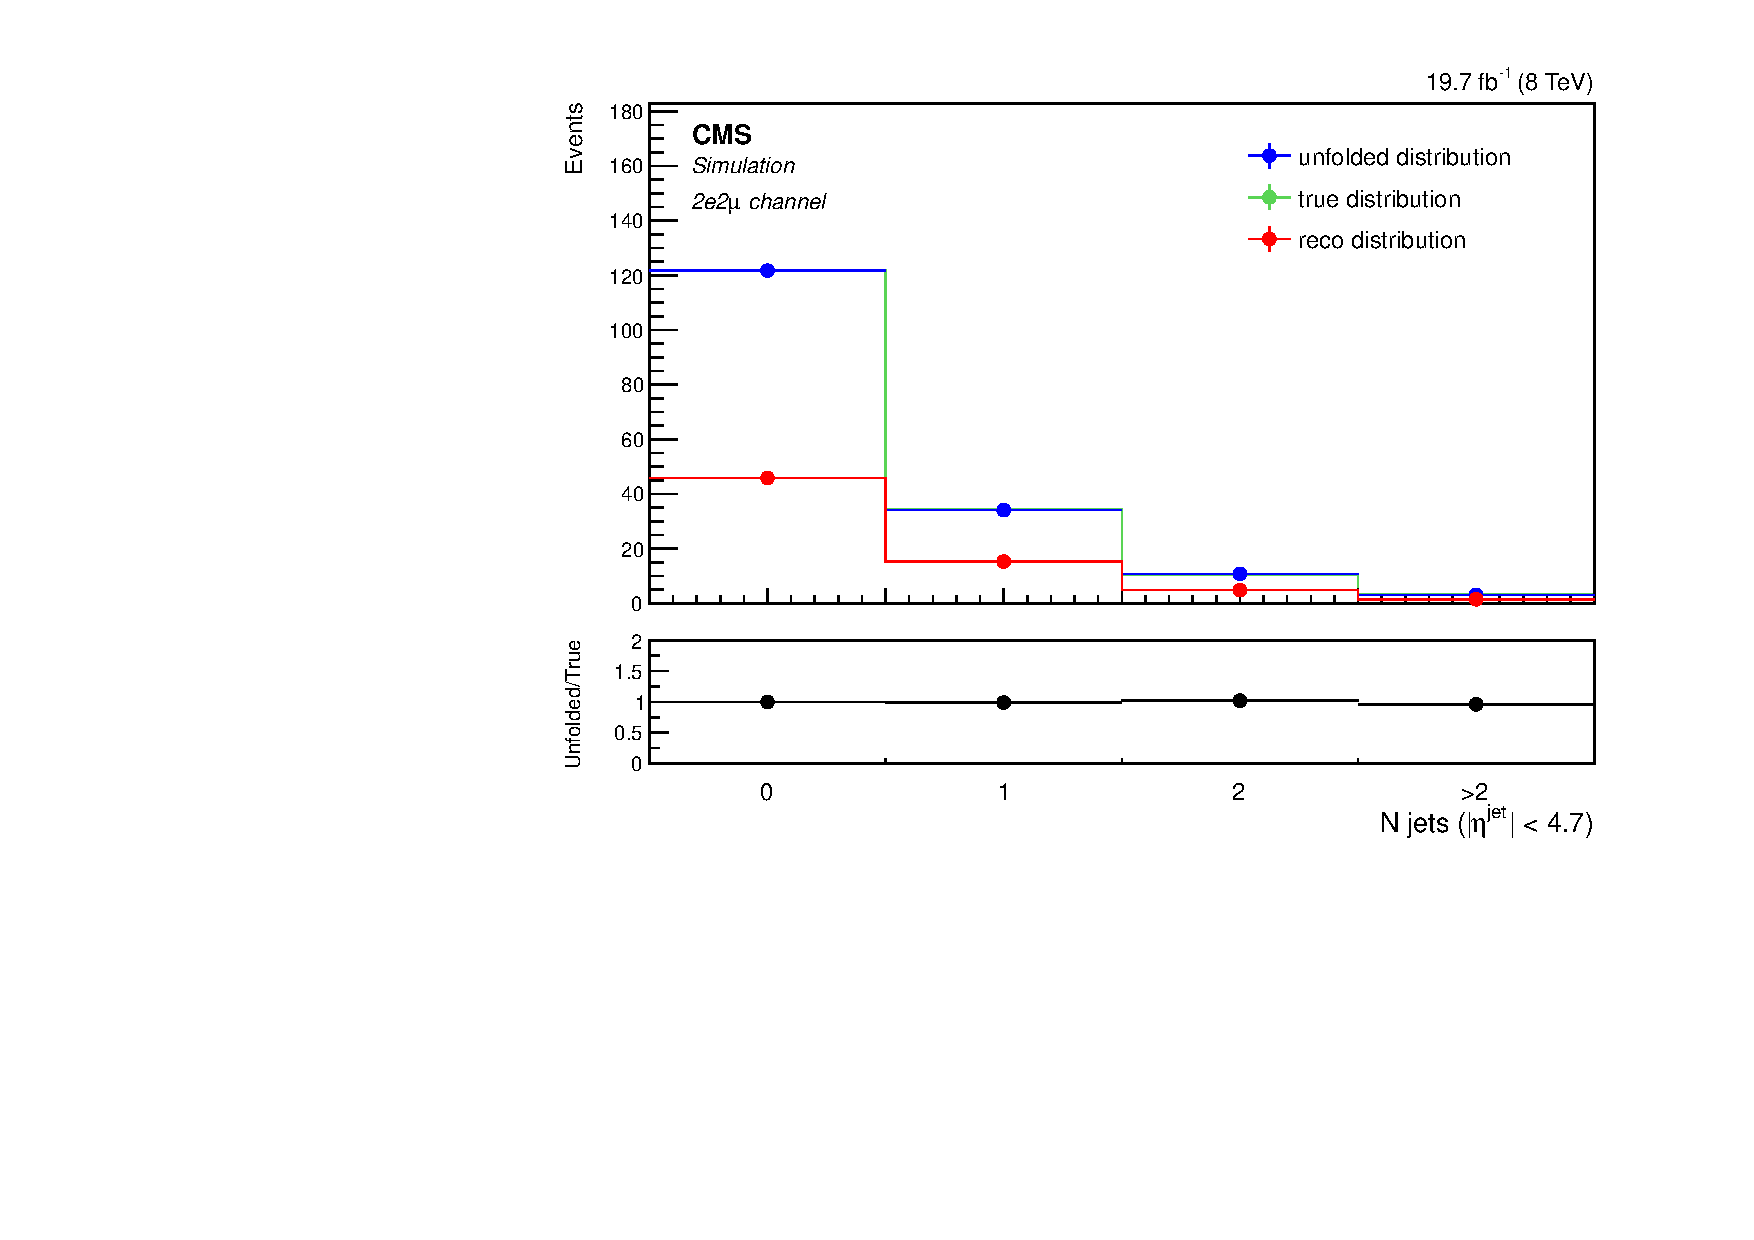
\includegraphics[width=\cmsFigWidth]{Figures/Unfolding/MCTests/Jets_ZZTo2e2m_MadMatrix_MadDistr_HalfSample}
%%      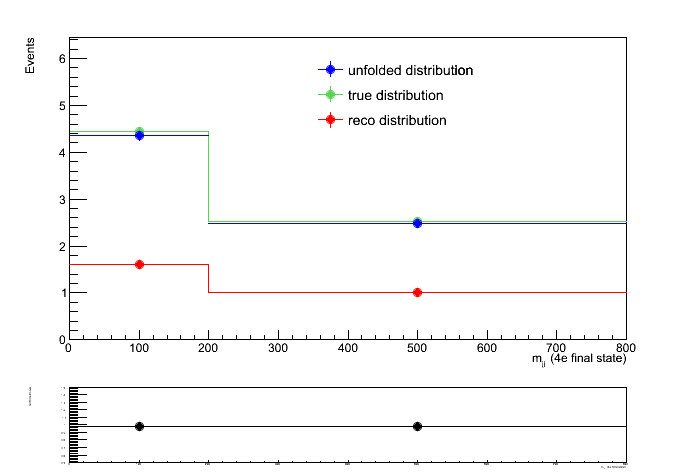
\includegraphics[width=\cmsFigWidth]{Figures/Unfolding/MCTests/Mjj_ZZTo4e_MadMatrix_MadDistr_HalfSample}
%%      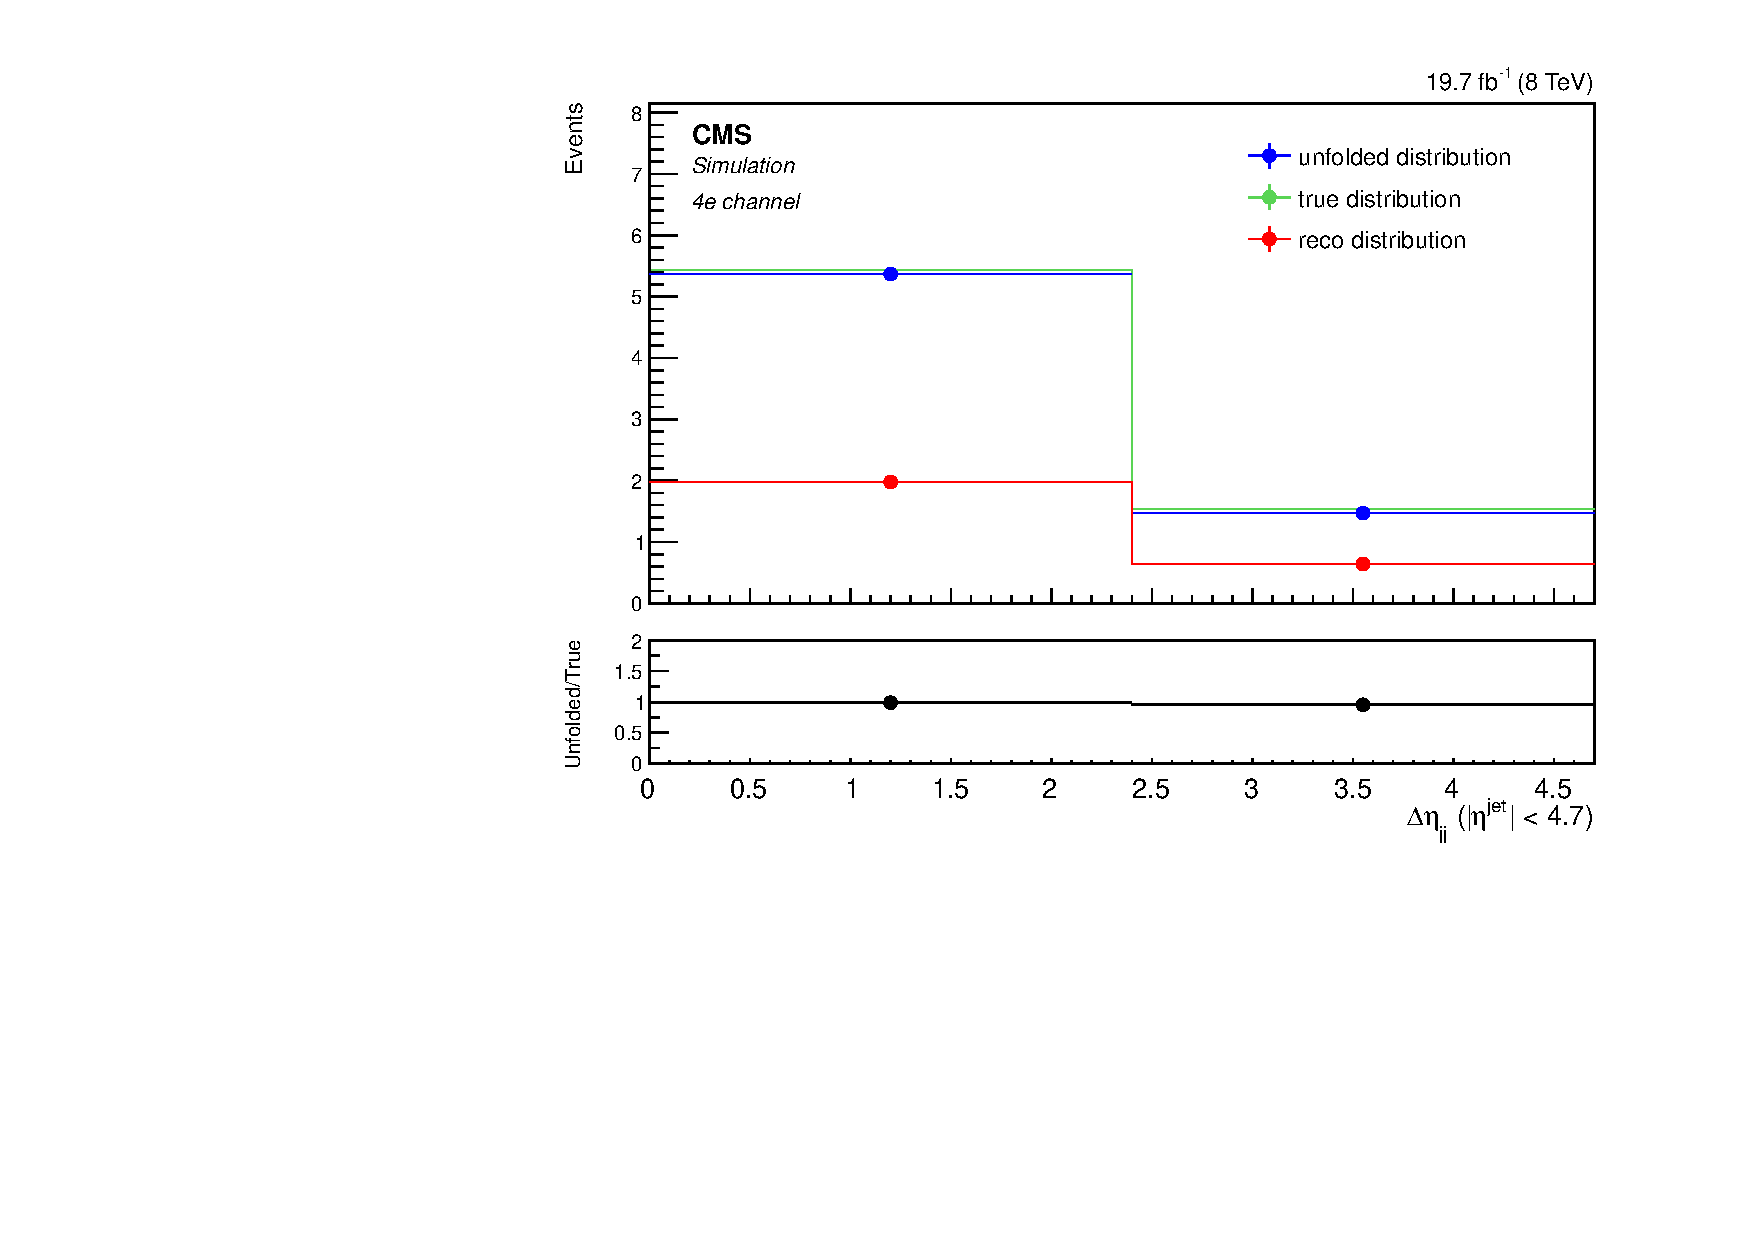
\includegraphics[width=\cmsFigWidth]{Figures/Unfolding/MCTests/Deta_ZZTo4e_MadMatrix_MadDistr_HalfSample}
%%      \caption{Unfolding test: \texttt{MadGraph} matrix applied on \texttt{MadGraph} distribution, using the two different halfs of the total sample. 
%%      Results are reported as a function of the invariant mass of the 4-lepton system (top left), the number of jets in the event (top right), the invariant mass of the
%%       two most energetic jets (bottom left) and the $\Delta\eta$ between them (bottom right) for the $2e2\mu$ final state.}
%%     \label{fig:HalfMad_2e2m}
%%   \end{center}
%% \end{figure}
%%     %%%%%%%%%%%%%%%%%%%%%%%%%%%%%%%%%%%%%%%%%%%%%%%%%%%%%%%%%%%%%%%%%%%%%%%%%%%%%%%%%%%%%%%%%%%%%%%%%%%%%%%%%%%%%%%%%%%%%%%%%%%%%%%%

%% \begin{figure}[hbtp]
%%   \begin{center}
%%     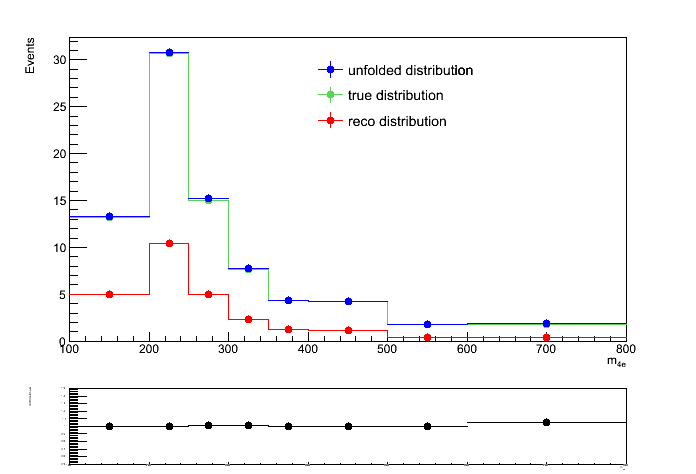
\includegraphics[width=\cmsFigWidth]{Figures/Unfolding/MCTests/Mass_ZZTo4e_PowMatrix_PowDistr_HalfSample}     
%%     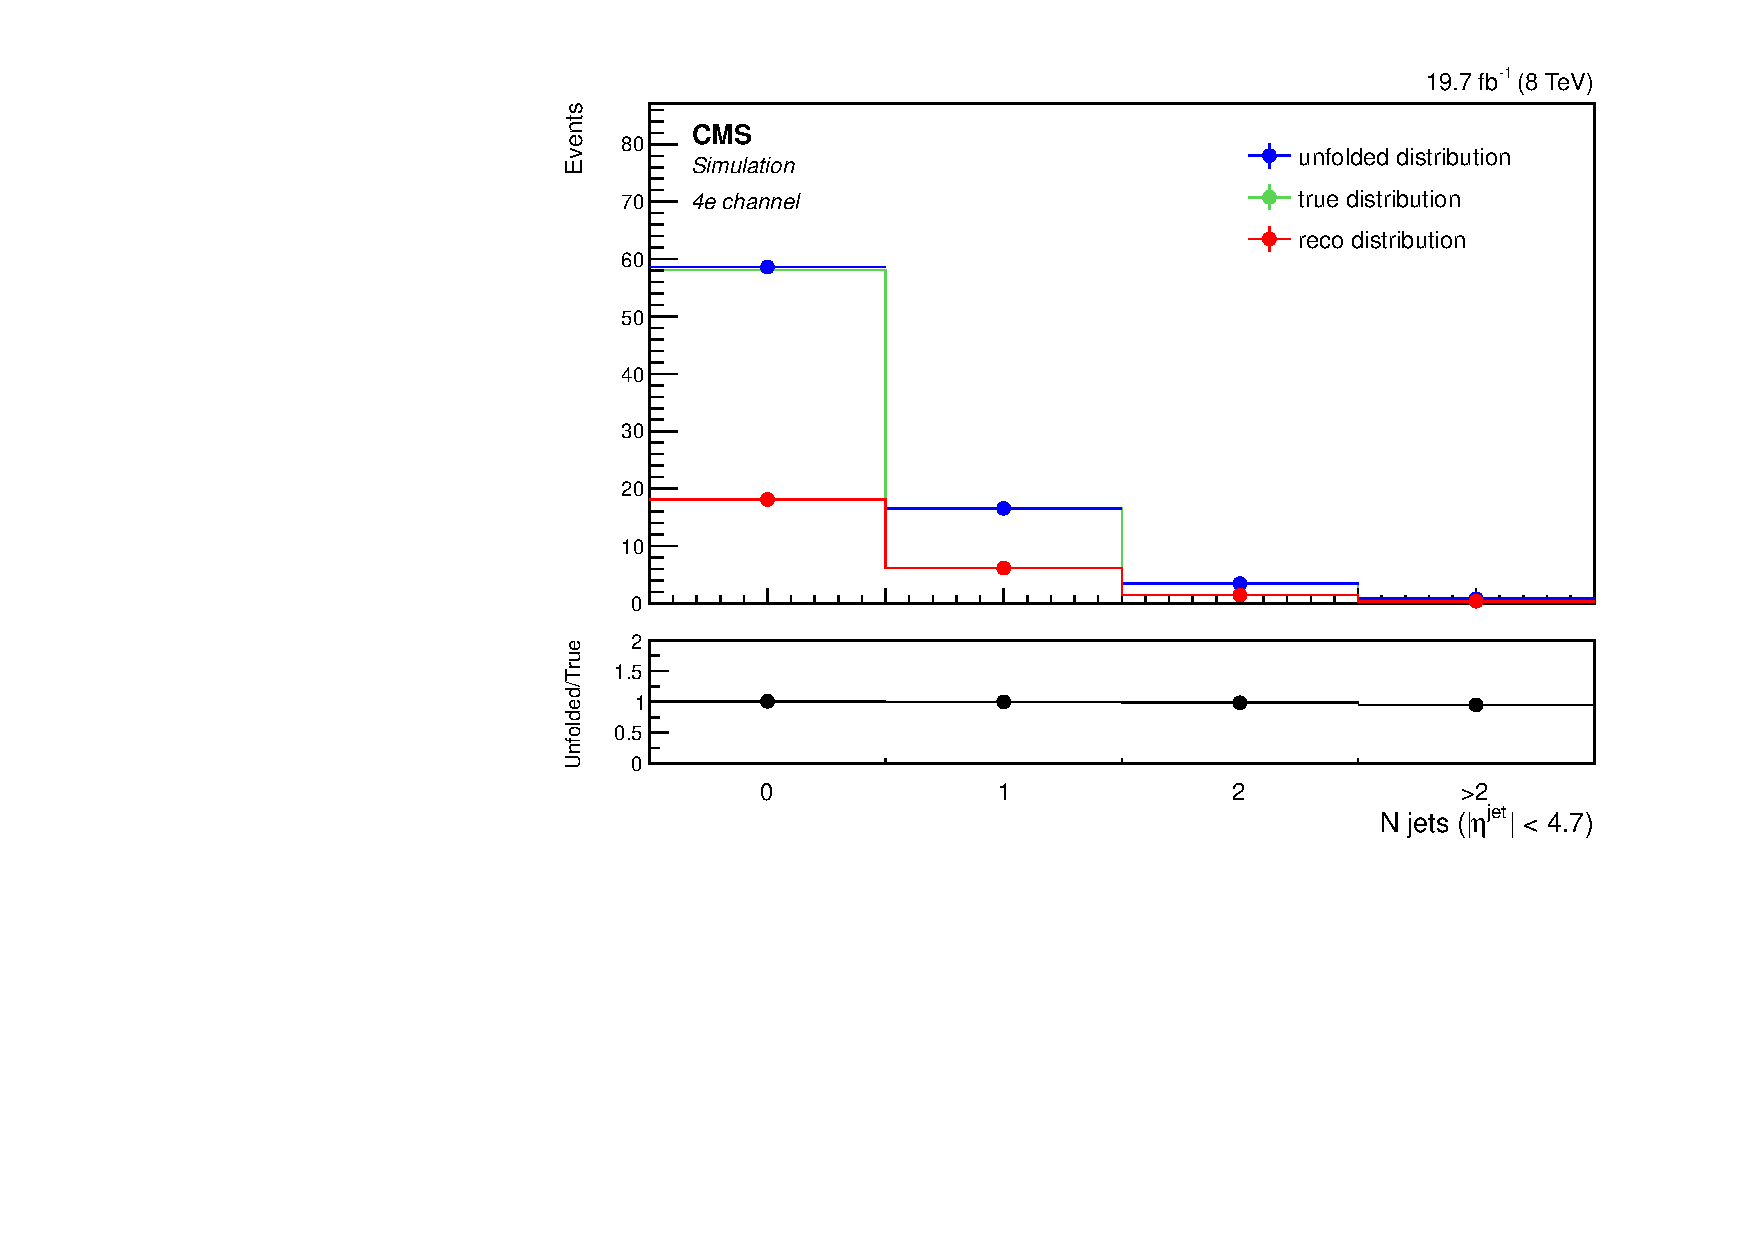
\includegraphics[width=\cmsFigWidth]{Figures/Unfolding/MCTests/Jets_ZZTo4e_PowMatrix_PowDistr_HalfSample}
%%      \includegraphics[width=\cmsFigWidth]{Figures/Unfolding/MCTests/Mjj_ZZTo4e_PowMatrix_PowDistr_HalfSample}
%%      \includegraphics[width=\cmsFigWidth]{Figures/Unfolding/MCTests/Deta_ZZTo4e_PowMatrix_PowDistr_HalfSample}
%%      \caption{Unfolding test: \texttt{Powheg} matrix applied on \texttt{Powheg} distribution, using the two different halfs of the total sample. 
%%      Results are reported as a function of the invariant mass of the 4-lepton system (top left), the number of jets in the event (top right), the invariant mass of the
%%       two most energetic jets (bottom left) and the $\Delta\eta$ between them (bottom right) for the $4e$ final state.}
%%     \label{fig:HalfPow_4e}
%%   \end{center}
%% \end{figure}
%% \begin{figure}[hbtp]
%%   \begin{center}
%%     \includegraphics[width=\cmsFigWidth]{Figures/Unfolding/MCTests/Mass_ZZTo4m_PowMatrix_PowDistr_HalfSample}     
%%     \includegraphics[width=\cmsFigWidth]{Figures/Unfolding/MCTests/Jets_ZZTo4m_PowMatrix_PowDistr_HalfSample}
%%      \includegraphics[width=\cmsFigWidth]{Figures/Unfolding/MCTests/Mjj_ZZTo4m_PowMatrix_PowDistr_HalfSample}
%%      \includegraphics[width=\cmsFigWidth]{Figures/Unfolding/MCTests/Deta_ZZTo4m_PowMatrix_PowDistr_HalfSample}
%%      \caption{Unfolding test: \texttt{Powheg} matrix applied on \texttt{Powheg} distribution, using the two different halfs of the total sample. 
%%      Results are reported as a function of the invariant mass of the 4-lepton system (top left), the number of jets in the event (top right), the invariant mass of the
%%       two most energetic jets (bottom left) and the $\Delta\eta$ between them (bottom right) for the $4\mu$ final state.}
%%     \label{fig:HalfPow_4m}
%%      \end{center}
%% \end{figure}
%% \begin{figure}[hbtp]
%%   \begin{center}
%%     \includegraphics[width=\cmsFigWidth]{Figures/Unfolding/MCTests/Mass_ZZTo2e2m_PowMatrix_PowDistr_HalfSample}     
%%     \includegraphics[width=\cmsFigWidth]{Figures/Unfolding/MCTests/Jets_ZZTo2e2m_PowMatrix_PowDistr_HalfSample}
%%      \includegraphics[width=\cmsFigWidth]{Figures/Unfolding/MCTests/Mjj_ZZTo4e_PowMatrix_PowDistr_HalfSample}
%%      \includegraphics[width=\cmsFigWidth]{Figures/Unfolding/MCTests/Deta_ZZTo4e_PowMatrix_PowDistr_HalfSample}
%%      \caption{Unfolding test: \texttt{Powheg} matrix applied on \texttt{Powheg} distribution, using the two different halfs of the total sample. 
%%      Results are reported as a function of the invariant mass of the 4-lepton system (top left), the number of jets in the event (top right), the invariant mass of the
%%       two most energetic jets (bottom left) and the $\Delta\eta$ between them (bottom right) for the $2e2\mu$ final state.}
%%     \label{fig:HalfPow_2e2m}
%%   \end{center}
%% \end{figure}

%% \begin{figure}[hbtp]
%%   \begin{center}
%%     \includegraphics[width=\cmsFigWidth]{Figures/Unfolding/MCTests/Mass_ZZTo4e_MadMatrix_PowDistr_FullSample}     
%%     \includegraphics[width=\cmsFigWidth]{Figures/Unfolding/MCTests/Jets_ZZTo4e_MadMatrix_PowDistr_FullSample}
%%      \includegraphics[width=\cmsFigWidth]{Figures/Unfolding/MCTests/Mjj_ZZTo4e_MadMatrix_PowDistr_FullSample}
%%      \includegraphics[width=\cmsFigWidth]{Figures/Unfolding/MCTests/Deta_ZZTo4e_MadMatrix_PowDistr_FullSample}
%%      \caption{Unfolding test: \texttt{MadGraph} matrix applied on \texttt{Powheg} distribution, using the two full samples. 
%%      Results are reported as a function of the invariant mass of the 4-lepton system (top left), the number of jets in the event (top right), the invariant mass of the
%%       two most energetic jets (bottom left) and the $\Delta\eta$ between them (bottom right) for the $4e$ final state.}
%%     \label{fig:MadMat_PowDist_4e}
%%   \end{center}
%% \end{figure}

%% \begin{figure}[hbtp]
%%   \begin{center}
%%     \includegraphics[width=\cmsFigWidth]{Figures/Unfolding/MCTests/Mass_ZZTo4m_MadMatrix_PowDistr_FullSample}     
%%     \includegraphics[width=\cmsFigWidth]{Figures/Unfolding/MCTests/Jets_ZZTo4m_MadMatrix_PowDistr_FullSample}
%%      \includegraphics[width=\cmsFigWidth]{Figures/Unfolding/MCTests/Mjj_ZZTo4m_MadMatrix_PowDistr_FullSample}
%%      \includegraphics[width=\cmsFigWidth]{Figures/Unfolding/MCTests/Deta_ZZTo4m_MadMatrix_PowDistr_FullSample}
%%      \caption{Unfolding test: \texttt{MadGraph} matrix applied on \texttt{Powheg} distribution, using the two full samples. 
%%      Results are reported as a function of the invariant mass of the 4-lepton system (top left), the number of jets in the event (top right), the invariant mass of the
%%       two most energetic jets (bottom left) and the $\Delta\eta$ between them (bottom right) for the $4\mu$ final state.}
%%     \label{fig:MadMat_PowDist_4m}
%%   \end{center}
%% \end{figure}

%% \begin{figure}[hbtp]
%%   \begin{center}
%%     \includegraphics[width=\cmsFigWidth]{Figures/Unfolding/MCTests/Mass_ZZTo2e2m_MadMatrix_PowDistr_FullSample}     
%%     \includegraphics[width=\cmsFigWidth]{Figures/Unfolding/MCTests/Jets_ZZTo2e2m_MadMatrix_PowDistr_FullSample}
%%     \includegraphics[width=\cmsFigWidth]{Figures/Unfolding/MCTests/Mjj_ZZTo4e_MadMatrix_PowDistr_FullSample}
%%     \includegraphics[width=\cmsFigWidth]{Figures/Unfolding/MCTests/Deta_ZZTo4e_MadMatrix_PowDistr_FullSample}
%%     \caption{Unfolding test: \texttt{MadGraph} matrix applied on \texttt{Powheg} distribution, using the two full samples. 
%%      Results are reported as a function of the invariant mass of the 4-lepton system (top left), the number of jets in the event (top right), the invariant mass of the
%%       two most energetic jets (bottom left) and the $\Delta\eta$ between them (bottom right) for the $2e2\mu$ final state.}
%%     \label{fig:MadMat_PowDist_2e2m}
%%   \end{center}
%% \end{figure}

%% \begin{figure}[hbtp]
%%   \begin{center}
%%     \includegraphics[width=\cmsFigWidth]{Figures/Unfolding/MCTests/Mass_ZZTo4e_PowMatrix_MadDistr_FullSample}     
%%     \includegraphics[width=\cmsFigWidth]{Figures/Unfolding/MCTests/Jets_ZZTo4e_PowMatrix_MadDistr_FullSample}
%%     \includegraphics[width=\cmsFigWidth]{Figures/Unfolding/MCTests/Mjj_ZZTo4e_PowMatrix_MadDistr_FullSample}
%%     \includegraphics[width=\cmsFigWidth]{Figures/Unfolding/MCTests/Deta_ZZTo4e_PowMatrix_MadDistr_FullSample}
%%     \caption{Unfolding test: \texttt{Powheg} matrix applied on \texttt{Matrix} distribution, using the two full samples. 
%%      Results are reported as a function of the invariant mass of the 4-lepton system (top left), the number of jets in the event (top right), the invariant mass of the
%%       two most energetic jets (bottom left) and the $\Delta\eta$ between them (bottom right) for the $4e$ final state.}
%%     \label{fig:PowMat_MadDist_4e}
%%   \end{center}
%% \end{figure}

%% \begin{figure}[hbtp]
%%   \begin{center}
%%     \includegraphics[width=\cmsFigWidth]{Figures/Unfolding/MCTests/Mass_ZZTo4m_PowMatrix_MadDistr_FullSample}     
%%     \includegraphics[width=\cmsFigWidth]{Figures/Unfolding/MCTests/Jets_ZZTo4m_PowMatrix_MadDistr_FullSample}
%%     \includegraphics[width=\cmsFigWidth]{Figures/Unfolding/MCTests/Mjj_ZZTo4m_PowMatrix_MadDistr_FullSample}
%%     \includegraphics[width=\cmsFigWidth]{Figures/Unfolding/MCTests/Deta_ZZTo4m_PowMatrix_MadDistr_FullSample}
%%     \caption{Unfolding test: \texttt{Powheg} matrix applied on \texttt{Matrix} distribution, using the two full samples. 
%%      Results are reported as a function of the invariant mass of the 4-lepton system (top left), the number of jets in the event (top right), the invariant mass o
%% the two most energetic jets (bottom left) and the $\Delta\eta$ between them (bottom right) for the $4\mu$ final state.}
%%     \label{fig:PowMat_MadDist_4m}
%%   \end{center}
%% \end{figure}

%% \begin{figure}[hbtp]
%%   \begin{center}
%%     \includegraphics[width=\cmsFigWidth]{Figures/Unfolding/MCTests/Mass_ZZTo2e2m_PowMatrix_MadDistr_FullSample}     
%%     \includegraphics[width=\cmsFigWidth]{Figures/Unfolding/MCTests/Jets_ZZTo2e2m_PowMatrix_MadDistr_FullSample}
%%     \includegraphics[width=\cmsFigWidth]{Figures/Unfolding/MCTests/Mjj_ZZTo4e_PowMatrix_MadDistr_FullSample}
%%     \includegraphics[width=\cmsFigWidth]{Figures/Unfolding/MCTests/Deta_ZZTo4e_PowMatrix_MadDistr_FullSample}
%%     \caption{Unfolding test: \texttt{Powheg} matrix applied on \texttt{Matrix} distribution, using the two full samples. 
%%      Results are reported as a function of the invariant mass of the 4-lepton system (top left), the number of jets in the event (top right), the invariant mass of
%%  the two most energetic jets (bottom left) and the $\Delta\eta$ between them (bottom right) for the $2e2\mu$ final state.}
%%     \label{fig:PowMat_MadDist_2e2mbis}
%%   \end{center}
%% \end{figure}




%%\begin{figure}[hbtp]
%%  \begin{center}
%%    \includegraphics[width=0.8\cmsFigWidth]{Figures/Unfolding/MCTests/Biased_Distributions/ZZTo4e_Mass_SVD2}     
%%    \includegraphics[width=0.8\cmsFigWidth]{Figures/Unfolding/MCTests/Biased_Distributions/ZZTo4m_Mass_SVD2}     
%%    \includegraphics[width=0.8\cmsFigWidth]{Figures/Unfolding/MCTests/Biased_Distributions/ZZTo2e2m_Mass_SVD2}
%%    \includegraphics[width=0.8\cmsFigWidth]{Figures/Unfolding/MCTests/Biased_Distributions/ZZTo4e_Mass_SVD4}     
%%    \includegraphics[width=0.8\cmsFigWidth]{Figures/Unfolding/MCTests/Biased_Distributions/ZZTo4m_Mass_SVD4}     
%%    \includegraphics[width=0.8\cmsFigWidth]{Figures/Unfolding/MCTests/Biased_Distributions/ZZTo2e2m_Mass_SVD4}
%%    \includegraphics[width=0.8\cmsFigWidth]{Figures/Unfolding/MCTests/Biased_Distributions/ZZTo4e_Mass_Bayes2}     
%%    \includegraphics[width=0.8\cmsFigWidth]{Figures/Unfolding/MCTests/Biased_Distributions/ZZTo4m_Mass_Bayes2}     
%%    \includegraphics[width=0.8\cmsFigWidth]{Figures/Unfolding/MCTests/Biased_Distributions/ZZTo2e2m_Mass_Bayes2}
%%     \caption{A flat distribution (in red) is unfolded using the SVD algorithm with $k_{reg} = 2$ (top) and $k_{reg} = 4$ (middle) and using the D'Agostini method with 4 iterations (bottom). Results are reported as a function of the invariant mass of the 4-lepton system  and for the $4e$ (left), $4\mu$ (center) and $2e2\mu$ (right) final state.}
%%    \label{fig:Mass_biased}
%%  \end{center}
%% \end{figure}

%% \begin{figure}[hbtp]
%%   \begin{center}
%%     \includegraphics[width=0.8\cmsFigWidth]{Figures/Unfolding/MCTests/Biased_Distributions/ZZTo4e_Jets_SVD2}     
%%     \includegraphics[width=0.8\cmsFigWidth]{Figures/Unfolding/MCTests/Biased_Distributions/ZZTo4m_Jets_SVD2}     
%%     \includegraphics[width=0.8\cmsFigWidth]{Figures/Unfolding/MCTests/Biased_Distributions/ZZTo2e2m_Jets_SVD2}
%%     \includegraphics[width=0.8\cmsFigWidth]{Figures/Unfolding/MCTests/Biased_Distributions/ZZTo4e_Jets_SVD4}     
%%     \includegraphics[width=0.8\cmsFigWidth]{Figures/Unfolding/MCTests/Biased_Distributions/ZZTo4m_Jets_SVD4}     
%%     \includegraphics[width=0.8\cmsFigWidth]{Figures/Unfolding/MCTests/Biased_Distributions/ZZTo2e2m_Jets_SVD4}
%%     \includegraphics[width=0.8\cmsFigWidth]{Figures/Unfolding/MCTests/Biased_Distributions/ZZTo4e_Jets_Bayes2}     
%%     \includegraphics[width=0.8\cmsFigWidth]{Figures/Unfolding/MCTests/Biased_Distributions/ZZTo4m_Jets_Bayes2}     
%%     \includegraphics[width=0.8\cmsFigWidth]{Figures/Unfolding/MCTests/Biased_Distributions/ZZTo2e2m_Jets_Bayes2}
%%      \caption{A flat distribution (in red) is unfolded using the SVD algorithm with $k_{reg} = 2$ (top) and $k_{reg} = 4$ (middle) and using the D'Agostini method with 4 iterations (bottom). Results are reported as a function of the number of jets and for the $4e$ (left), $4\mu$ (center) and $2e2\mu$ (right) final state.}
%%     \label{fig:Jets_biased}
%%   \end{center}
%% \end{figure}


\begin{figure}[hbtp]
 \begin{center}
    \includegraphics[width=0.8\cmsFigWidth]{Figures/Unfolding/Systematics/ZZTo4e_Mass_qqgg}     
    \includegraphics[width=0.8\cmsFigWidth]{Figures/Unfolding/Systematics/ZZTo4e_Mass_MCgen}     
    \includegraphics[width=0.8\cmsFigWidth]{Figures/Unfolding/Systematics/ZZTo4e_Mass_IrrBkg}
    \includegraphics[width=0.8\cmsFigWidth]{Figures/Unfolding/Systematics/ZZTo4e_Mass_RedBkg}     
    \includegraphics[width=0.8\cmsFigWidth]{Figures/Unfolding/Systematics/ZZTo4e_Mass_UnfDataOverGenMC}     
    %\includegraphics[width=0.8\cmsFigWidth]{Figures/Unfolding/Systematics/ZZTo4e_Mass_JER}
   % \includegraphics[width=0.8\cmsFigWidth]{Figures/Unfolding/Systematics/ZZTo4e_Mass_JES_ModData}     
   % \includegraphics[width=0.8\cmsFigWidth]{Figures/Unfolding/Systematics/ZZTo4e_Mass_JES_ModMat}
    \caption{Effects of the different sources of systematic uncertainty on the unfolded distributions of the number of jets, for the     
    $4e$ final state. From left to right, from top to bottom: $\sigma_{qq}$ and $\sigma_{gg}$ ratio, MC generator, irreducible background,
reducible background, data/MC ratio. The shifted distributions due to the systematic effects are reported, together with the nominal one and
the MC truth.}
    \label{fig:Mass_syst_4e}
  \end{center}
\end{figure}

\begin{figure}[hbtp]
  \begin{center}
    \includegraphics[width=0.8\cmsFigWidth]{Figures/Unfolding/Systematics/ZZTo4m_Mass_qqgg}     
    \includegraphics[width=0.8\cmsFigWidth]{Figures/Unfolding/Systematics/ZZTo4m_Mass_MCgen}     
    \includegraphics[width=0.8\cmsFigWidth]{Figures/Unfolding/Systematics/ZZTo4m_Mass_IrrBkg}
    \includegraphics[width=0.8\cmsFigWidth]{Figures/Unfolding/Systematics/ZZTo4m_Mass_RedBkg}     
    \includegraphics[width=0.8\cmsFigWidth]{Figures/Unfolding/Systematics/ZZTo4m_Mass_UnfDataOverGenMC}     
   % \includegraphics[width=0.8\cmsFigWidth]{Figures/Unfolding/Systematics/ZZTo4m_Mass_JER}
    %\includegraphics[width=0.8\cmsFigWidth]{Figures/Unfolding/Systematics/ZZTo4m_Mass_JES_ModData}     
   % \includegraphics[width=0.8\cmsFigWidth]{Figures/Unfolding/Systematics/ZZTo4m_Mass_JES_ModMat}
    \caption{Effects of the different sources of systematic uncertainty on the unfolded distributions of the number of jets, for the     
    $4\mu$ final state. From left to right, from top to bottom: $\sigma_{qq}$ and $\sigma_{gg}$ ratio, MC generator, irreducible background,
reducible background, data/MC ratio The shifted distributions due to the systematic effects are reported, together with the nominal one and
the MC truth.}
    \label{fig:Mass_syst_4m}
  \end{center}
\end{figure}

\begin{figure}[hbtp]
  \begin{center}
    \includegraphics[width=0.8\cmsFigWidth]{Figures/Unfolding/Systematics/ZZTo2e2m_Mass_qqgg}     
    \includegraphics[width=0.8\cmsFigWidth]{Figures/Unfolding/Systematics/ZZTo2e2m_Mass_MCgen}     
    \includegraphics[width=0.8\cmsFigWidth]{Figures/Unfolding/Systematics/ZZTo2e2m_Mass_IrrBkg}
    \includegraphics[width=0.8\cmsFigWidth]{Figures/Unfolding/Systematics/ZZTo2e2m_Mass_RedBkg}     
    \includegraphics[width=0.8\cmsFigWidth]{Figures/Unfolding/Systematics/ZZTo2e2m_Mass_UnfDataOverGenMC}     
   % \includegraphics[width=0.8\cmsFigWidth]{Figures/Unfolding/Systematics/ZZTo2e2m_Mass_JER}
   % \includegraphics[width=0.8\cmsFigWidth]{Figures/Unfolding/Systematics/ZZTo2e2m_Mass_JES_ModData}     
  % \includegraphics[width=0.8\cmsFigWidth]{Figures/Unfolding/Systematics/ZZTo2e2m_Mass_JES_ModMat}
    \caption{Effects of the different sources of systematic uncertainty on the unfolded distributions of the number of jets, for the     
    $2e2\mu$ final state. From left to right, from top to bottom: $\sigma_{qq}$ and $\sigma_{gg}$ ratio, MC generator, irreducible background,
reducible background, data/MC ratio The shifted distributions due to the systematic effects are reported, together with the nominal one and
the MC truth.}
    \label{fig:Mass_syst_2e2m}
  \end{center}
\end{figure}

\begin{figure}[hbtp]
  \begin{center}
    \includegraphics[width=0.8\cmsFigWidth]{Figures/Unfolding/Systematics/ZZTo4e_Jets_qqgg}     
    \includegraphics[width=0.8\cmsFigWidth]{Figures/Unfolding/Systematics/ZZTo4e_Jets_MCgen}     
    \includegraphics[width=0.8\cmsFigWidth]{Figures/Unfolding/Systematics/ZZTo4e_Jets_IrrBkg}
    \includegraphics[width=0.8\cmsFigWidth]{Figures/Unfolding/Systematics/ZZTo4e_Jets_RedBkg}     
    \includegraphics[width=0.8\cmsFigWidth]{Figures/Unfolding/Systematics/ZZTo4e_Jets_UnfDataOverGenMC}     
    \includegraphics[width=0.8\cmsFigWidth]{Figures/Unfolding/Systematics/ZZTo4e_Jets_JER}
    \includegraphics[width=0.8\cmsFigWidth]{Figures/Unfolding/Systematics/ZZTo4e_Jets_JES_ModData}     
    \includegraphics[width=0.8\cmsFigWidth]{Figures/Unfolding/Systematics/ZZTo4e_Jets_JES_ModMat}
    \caption{Effects of the different sources of systematic uncertainty on the unfolded distributions of the number of jets, for the     
    $4e$ final state. From left to right, from top to bottom: $\sigma_{qq}$ and $\sigma_{gg}$ ratio, MC generator, irreducible background,
reducible background, data/MC ratio, JER, JES modifying data distribution, JES modifying the response matrix The shifted distributions due to the systematic effects are reported, together with the nominal one and
the MC truth.}
    \label{fig:Jets_syst_4e}
  \end{center}
\end{figure}

\begin{figure}[hbtp]
  \begin{center}
    \includegraphics[width=0.8\cmsFigWidth]{Figures/Unfolding/Systematics/ZZTo4m_Jets_qqgg}     
    \includegraphics[width=0.8\cmsFigWidth]{Figures/Unfolding/Systematics/ZZTo4m_Jets_MCgen}     
    \includegraphics[width=0.8\cmsFigWidth]{Figures/Unfolding/Systematics/ZZTo4m_Jets_IrrBkg}
    \includegraphics[width=0.8\cmsFigWidth]{Figures/Unfolding/Systematics/ZZTo4m_Jets_RedBkg}     
    \includegraphics[width=0.8\cmsFigWidth]{Figures/Unfolding/Systematics/ZZTo4m_Jets_UnfDataOverGenMC}     
    \includegraphics[width=0.8\cmsFigWidth]{Figures/Unfolding/Systematics/ZZTo4m_Jets_JER}
    \includegraphics[width=0.8\cmsFigWidth]{Figures/Unfolding/Systematics/ZZTo4m_Jets_JES_ModData}     
    \includegraphics[width=0.8\cmsFigWidth]{Figures/Unfolding/Systematics/ZZTo4m_Jets_JES_ModMat}
    \caption{Effects of the different sources of systematic uncertainty on the unfolded distributions of the number of jets, for the     
    $4\mu$ final state. From left to right, from top to bottom: $\sigma_{qq}$ and $\sigma_{gg}$ ratio, MC generator, irreducible background,
reducible background, data/MC ratio, JER, JES modifying data distribution, JES modifying the response matrix The shifted distributions due to the systematic effects are reported, together with the nominal one and
the MC truth.}
    \label{fig:Jets_syst_4m}
  \end{center}
\end{figure}

\begin{figure}[hbtp]
  \begin{center}
    \includegraphics[width=0.8\cmsFigWidth]{Figures/Unfolding/Systematics/ZZTo2e2m_Jets_qqgg}     
    \includegraphics[width=0.8\cmsFigWidth]{Figures/Unfolding/Systematics/ZZTo2e2m_Jets_MCgen}     
    \includegraphics[width=0.8\cmsFigWidth]{Figures/Unfolding/Systematics/ZZTo2e2m_Jets_IrrBkg}
    \includegraphics[width=0.8\cmsFigWidth]{Figures/Unfolding/Systematics/ZZTo2e2m_Jets_RedBkg}     
    \includegraphics[width=0.8\cmsFigWidth]{Figures/Unfolding/Systematics/ZZTo2e2m_Jets_UnfDataOverGenMC}     
    \includegraphics[width=0.8\cmsFigWidth]{Figures/Unfolding/Systematics/ZZTo2e2m_Jets_JER}
    \includegraphics[width=0.8\cmsFigWidth]{Figures/Unfolding/Systematics/ZZTo2e2m_Jets_JES_ModData}     
    \includegraphics[width=0.8\cmsFigWidth]{Figures/Unfolding/Systematics/ZZTo2e2m_Jets_JES_ModMat}
    \caption{Effects of the different sources of systematic uncertainty on the unfolded distributions of the number of jets, for the     
    $2e2\mu$ final state. From left to right, from top to bottom: $\sigma_{qq}$ and $\sigma_{gg}$ ratio, MC generator, irreducible background,
reducible background, data/MC ratio, JER, JES modifying data distribution, JES modifying the response matrix The shifted distributions due to the systematic effects are reported, together with the nominal one and
the MC truth.}
    \label{fig:Jets_syst_2e2m}
  \end{center}
\end{figure}

\begin{figure}[hbtp]
  \begin{center}
    \includegraphics[width=0.8\cmsFigWidth]{Figures/Unfolding/Systematics/ZZTo4e_Mjj_qqgg}     
    \includegraphics[width=0.8\cmsFigWidth]{Figures/Unfolding/Systematics/ZZTo4e_Mjj_MCgen}     
    \includegraphics[width=0.8\cmsFigWidth]{Figures/Unfolding/Systematics/ZZTo4e_Mjj_IrrBkg}
    \includegraphics[width=0.8\cmsFigWidth]{Figures/Unfolding/Systematics/ZZTo4e_Mjj_RedBkg}     
    %\includegraphics[width=0.8\cmsFigWidth]{Figures/Unfolding/Systematics/ZZTo4e_Mjj_UnfDataOverGenMC}     
    \includegraphics[width=0.8\cmsFigWidth]{Figures/Unfolding/Systematics/ZZTo4e_Mjj_JER}
    \includegraphics[width=0.8\cmsFigWidth]{Figures/Unfolding/Systematics/ZZTo4e_Mjj_JES_ModData}     
    \includegraphics[width=0.8\cmsFigWidth]{Figures/Unfolding/Systematics/ZZTo4e_Mjj_JES_ModMat}
    \caption{Effects of the different sources of systematic uncertainty on the unfolded distributions of $m_{jj}$, for the     
    $4e$ final state. From left to right, from top to bottom: $\sigma_{qq}$ and $\sigma_{gg}$ ratio, MC generator, irreducible background,
reducible background, data/MC ratio, JER, JES modifying data distribution, JES modifying the response matrix The shifted distributions due to the systematic effects are reported, together with the nominal one and
the MC truth.}
    \label{fig:Mjj_syst_4e}
  \end{center}
\end{figure}

\begin{figure}[hbtp]
  \begin{center}
    \includegraphics[width=0.8\cmsFigWidth]{Figures/Unfolding/Systematics/ZZTo4m_Mjj_qqgg}     
    \includegraphics[width=0.8\cmsFigWidth]{Figures/Unfolding/Systematics/ZZTo4m_Mjj_MCgen}     
    \includegraphics[width=0.8\cmsFigWidth]{Figures/Unfolding/Systematics/ZZTo4m_Mjj_IrrBkg}
    \includegraphics[width=0.8\cmsFigWidth]{Figures/Unfolding/Systematics/ZZTo4m_Mjj_RedBkg}     
    %\includegraphics[width=0.8\cmsFigWidth]{Figures/Unfolding/Systematics/ZZTo4m_Mjj_UnfDataOverGenMC}     
    \includegraphics[width=0.8\cmsFigWidth]{Figures/Unfolding/Systematics/ZZTo4m_Mjj_JER}
    \includegraphics[width=0.8\cmsFigWidth]{Figures/Unfolding/Systematics/ZZTo4m_Mjj_JES_ModData}     
    \includegraphics[width=0.8\cmsFigWidth]{Figures/Unfolding/Systematics/ZZTo4m_Mjj_JES_ModMat}
    \caption{Effects of the different sources of systematic uncertainty on the unfolded distributions of $m_{jj}$, for the     
    $4\mu$ final state. From left to right, from top to bottom: $\sigma_{qq}$ and $\sigma_{gg}$ ratio, MC generator, irreducible background,
reducible background, data/MC ratio, JER, JES modifying data distribution, JES modifying the response matrix The shifted distributions due to the systematic effects are reported, together with the nominal one and the MC truth.}
    \label{fig:Mjj_syst_4m}
  \end{center}
\end{figure}

\begin{figure}[hbtp]
  \begin{center}
    \includegraphics[width=0.8\cmsFigWidth]{Figures/Unfolding/Systematics/ZZTo2e2m_Mjj_qqgg}     
    \includegraphics[width=0.8\cmsFigWidth]{Figures/Unfolding/Systematics/ZZTo2e2m_Mjj_MCgen}     
    \includegraphics[width=0.8\cmsFigWidth]{Figures/Unfolding/Systematics/ZZTo2e2m_Mjj_IrrBkg}
    \includegraphics[width=0.8\cmsFigWidth]{Figures/Unfolding/Systematics/ZZTo2e2m_Mjj_RedBkg}     
   % \includegraphics[width=0.8\cmsFigWidth]{Figures/Unfolding/Systematics/ZZTo2e2m_Mjj_UnfDataOverGenMC}     
    \includegraphics[width=0.8\cmsFigWidth]{Figures/Unfolding/Systematics/ZZTo2e2m_Mjj_JER}
    \includegraphics[width=0.8\cmsFigWidth]{Figures/Unfolding/Systematics/ZZTo2e2m_Mjj_JES_ModData}     
    \includegraphics[width=0.8\cmsFigWidth]{Figures/Unfolding/Systematics/ZZTo2e2m_Mjj_JES_ModMat}
    \caption{Effects of the different sources of systematic uncertainty on the unfolded distributions of $m_{jj}$, for the     
    $2e2\mu$ final state. From left to right, from top to bottom: $\sigma_{qq}$ and $\sigma_{gg}$ ratio, MC generator, irreducible background,
reducible background, data/MC ratio, JER, JES modifying data distribution, JES modifying the response matrix The shifted distributions due to the systematic effects are reported, together with the nominal one and the MC truth.}
   \label{fig:Mjj_syst_2e2m}
  \end{center}
\end{figure}

\begin{figure}[hbtp]
 \begin{center}
   \includegraphics[width=0.8\cmsFigWidth]{Figures/Unfolding/Systematics/ZZTo4e_Deta_qqgg}     
   \includegraphics[width=0.8\cmsFigWidth]{Figures/Unfolding/Systematics/ZZTo4e_Deta_MCgen}     
   \includegraphics[width=0.8\cmsFigWidth]{Figures/Unfolding/Systematics/ZZTo4e_Deta_IrrBkg}
   \includegraphics[width=0.8\cmsFigWidth]{Figures/Unfolding/Systematics/ZZTo4e_Deta_RedBkg}     
   %\includegraphics[width=0.8\cmsFigWidth]{Figures/Unfolding/Systematics/ZZTo4e_Deta_UnfDataOverGenMC}     
   \includegraphics[width=0.8\cmsFigWidth]{Figures/Unfolding/Systematics/ZZTo4e_Deta_JER}
   \includegraphics[width=0.8\cmsFigWidth]{Figures/Unfolding/Systematics/ZZTo4e_Deta_JES_ModData}     
   \includegraphics[width=0.8\cmsFigWidth]{Figures/Unfolding/Systematics/ZZTo4e_Deta_JES_ModMat}
   \caption{Effects of the different sources of systematic uncertainty on the unfolded distributions of $\Delta\eta_{jj}$, for the     
   $4e$ final state. From left to right, from top to bottom: $\sigma_{qq}$ and $\sigma_{gg}$ ratio, MC generator, irreducible background,
reducible background, data/MC ratio, JER, JES modifying data distribution, JES modifying the response matrix The shifted distributions due to the systematic effects are reported, together with the nominal one and
the MC truth.}
   \label{fig:Deta_syst_4e}
 \end{center}
\end{figure}

\begin{figure}[hbtp]
 \begin{center}
   \includegraphics[width=0.8\cmsFigWidth]{Figures/Unfolding/Systematics/ZZTo4m_Deta_qqgg}     
   \includegraphics[width=0.8\cmsFigWidth]{Figures/Unfolding/Systematics/ZZTo4m_Deta_MCgen}     
   \includegraphics[width=0.8\cmsFigWidth]{Figures/Unfolding/Systematics/ZZTo4m_Deta_IrrBkg}
   \includegraphics[width=0.8\cmsFigWidth]{Figures/Unfolding/Systematics/ZZTo4m_Deta_RedBkg}     
   %\includegraphics[width=0.8\cmsFigWidth]{Figures/Unfolding/Systematics/ZZTo4m_Deta_UnfDataOverGenMC}     
   \includegraphics[width=0.8\cmsFigWidth]{Figures/Unfolding/Systematics/ZZTo4m_Deta_JER}
   \includegraphics[width=0.8\cmsFigWidth]{Figures/Unfolding/Systematics/ZZTo4m_Deta_JES_ModData}     
   \includegraphics[width=0.8\cmsFigWidth]{Figures/Unfolding/Systematics/ZZTo4m_Deta_JES_ModMat}
   \caption{Effects of the different sources of systematic uncertainty on the unfolded distributions of $\Delta\eta_{jj}$, for the     
   $4\mu$ final state. From left to right, from top to bottom: $\sigma_{qq}$ and $\sigma_{gg}$ ratio, MC generator, irreducible background,
reducible background, data/MC ratio, JER, JES modifying data distribution, JES modifying the response matrix The shifted distributions due to the systematic effects are reported, together with the nominal one and
the MC truth.}
   \label{fig:Deta_syst_4m}
 \end{center}
\end{figure}

\begin{figure}[hbtp]
 \begin{center}
   \includegraphics[width=0.8\cmsFigWidth]{Figures/Unfolding/Systematics/ZZTo2e2m_Deta_qqgg}     
   \includegraphics[width=0.8\cmsFigWidth]{Figures/Unfolding/Systematics/ZZTo2e2m_Deta_MCgen}     
   \includegraphics[width=0.8\cmsFigWidth]{Figures/Unfolding/Systematics/ZZTo2e2m_Deta_IrrBkg}
   \includegraphics[width=0.8\cmsFigWidth]{Figures/Unfolding/Systematics/ZZTo2e2m_Deta_RedBkg}     
   %\includegraphics[width=0.8\cmsFigWidth]{Figures/Unfolding/Systematics/ZZTo2e2m_Deta_UnfDataOverGenMC}     
   \includegraphics[width=0.8\cmsFigWidth]{Figures/Unfolding/Systematics/ZZTo2e2m_Deta_JER}
   \includegraphics[width=0.8\cmsFigWidth]{Figures/Unfolding/Systematics/ZZTo2e2m_Deta_JES_ModData}     
   \includegraphics[width=0.8\cmsFigWidth]{Figures/Unfolding/Systematics/ZZTo2e2m_Deta_JES_ModMat}
   \caption{Effects of the different sources of systematic uncertainty on the unfolded distributions of $\Delta\eta_{jj}$, for the     
   $2e2\mu$ final state. From left to right, from top to bottom: $\sigma_{qq}$ and $\sigma_{gg}$ ratio, MC generator, irreducible background,
reducible background, data/MC ratio, JER, JES modifying data distribution, JES modifying the response matrix The shifted distributions due to the systematic effects are reported, together with the nominal one and
the MC truth.}
   \label{fig:Detasyst2e2m}
 \end{center}
\end{figure}
